
\documentclass[a4paper,12pt,openany,oneside]{book}  

% ==========================================
% 1. PAQUETES (Librerías)
% ==========================================

% --- Codificación e Idioma ---
\usepackage[utf8]{inputenc}
\usepackage[spanish,es-tabla]{babel}

% --- Gráficos y Figuras ---
\usepackage{graphicx} 
\usepackage{tikz,color}
\usepackage{pgf-pie} 
\usepackage{wrapfig}    
\usepackage[scriptsize]{caption} 
\usepackage{subcaption}
\usepackage{float}    
\usepackage{adjustbox}


\usepackage{amsmath} 
\usepackage{amsthm}  
\usepackage{amssymb}
\usepackage{mathtools}
\usepackage{bm}

% --- Tablas (Fusionado) ---
\usepackage{array}
\usepackage{longtable}
\usepackage{booktabs}
\usepackage{tabularx}
\usepackage{multirow}
\usepackage{multicol}
\usepackage{rotating}
\usepackage{lscape}
\usepackage{csvsimple}
\usepackage[section]{placeins}

% --- Otros ---
\usepackage{lastpage}
\usepackage{pdfpages}
\usepackage{url}
\usepackage{eurosym}
\usepackage[ruled,noline,linesnumbered,spanish]{algorithm2e}
\usepackage{appendix}
\usepackage{epstopdf} 

% --- Hipervínculos 
\usepackage[hidelinks]{hyperref} 


\usepackage{listings}
\usepackage{xcolor}

\definecolor{codegreen}{rgb}{0,0.6,0}
\definecolor{codegray}{rgb}{0.5,0.5,0.5}
\definecolor{codepurple}{rgb}{0.58,0,0.82}
\definecolor{backcolour}{rgb}{0.95,0.95,0.92}

\lstdefinestyle{mystyle}{
    backgroundcolor=\color{backcolour},   
    commentstyle=\color{codegreen},
    keywordstyle=\color{magenta},
    numberstyle=\tiny\color{codegray},
    stringstyle=\color{codepurple},
    basicstyle=\ttfamily\footnotesize,
    breakatwhitespace=false,         
    breaklines=true,                 
    captionpos=b,                    
    keepspaces=true,                 
    numbers=left,                    
    numbersep=5pt,                  
    showspaces=false,                
    showstringspaces=false,
    showtabs=false,                  
    tabsize=2,
    literate={á}{{\'a}}1 {é}{{\'e}}1 {í}{{\'i}}1 {ó}{{\'o}}1 {ú}{{\'u}}1 {ñ}{{\~n}}1 % Para tildes en código
}

\lstset{style=mystyle}
\renewcommand{\lstlistingname}{Listado}


\renewcommand{\contentsname}{Índice de contenido}
\renewcommand{\chaptername}{Capítulo}            
\renewcommand{\bibname}{Referencias} 
\renewcommand{\listfigurename}{Índice de figuras}
\renewcommand{\listtablename}{Índice de tablas}
\renewcommand{\figurename}{Figura}
\renewcommand{\tablename}{Tabla}
\renewcommand{\arraystretch}{1.25}

% --- Algoritmos / Pseudocódigo ---
\SetKwInput{KwIn}{Entrada}
\SetKwInput{KwOut}{Salida}
\SetKwFor{For}{para}{hacer}{fin~para}
\SetAlgoNlRelativeSize{-1}
\SetAlCapSkip{0.5em}
\DontPrintSemicolon
\SetAlgoSkip{bigskip}

\addto\captionsspanish{\renewcommand{\appendixname}{Anexo}}
\renewcommand{\appendixtocname}{Anexos}
\renewcommand{\appendixpagename}{Anexos}


\newcolumntype{C}[1]{>{\centering\arraybackslash}m{#1}}
\providecommand{\keywords}[1]{\textbf{\textit{Keywords---}} #1}

\setlength{\parskip}{5pt}

\begin{document}


\pagestyle{empty}



\begin{center}
	\newcommand{\HRule}{\rule{\linewidth}{0.7mm}}
	\begin{center}
            
\includegraphics[width=\columnwidth, keepaspectratio]{imagenes/logo.png}\\
    \end{center}

	\vspace*{1cm}
	\textsc{\large Universidad de Extremadura}\\[0.5cm]
	\textsc{\large Centro Universitario de Mérida}\\[1.3cm]
	\textsc{\LARGE Grado en Ingeniería Telemática en Telecomunicación}\\[1.3cm]
	\textsc{\huge Trabajo Fin de Grado}\\[2cm]
	\textsc{\LARGE Estudio de cobertura 3D para redes celulares haciendo uso de modelo de antenas y canal de propagación. }\\[2 cm]
	
	\textsc{\large Francisco Montero Sánchez}
	\vspace{1.5cm} 
	\vfill
	Mérida, septiembre de 2026
\end{center}

\cleardoublepage
\pagestyle{empty}

\begin{center}
	\newcommand{\HRule}{\rule{\linewidth}{0.7mm}}
    
	\begin{center}
            
\includegraphics[width=\columnwidth, keepaspectratio]{imagenes/logo.png}\\
        \end{center}
	
	\vspace*{1cm}
	\textsc{\large Universidad de Extremadura}\\[0.5cm]
	\textsc{\large Centro Universitario de Mérida}\\[1.3cm]
	\textsc{\LARGE Grado en Ingeniería Telemática en Telecomunicación}\\[1.3cm]
	\textsc{\huge Trabajo Fin de Grado}\\[1.5 cm]
	\textsc{\LARGE Estudio de cobertura 3D para redes celulares haciendo uso de modelo de antenas y canal de propagación.}\\[1.5 cm]

\end{center}

\begin{flushleft}
\renewcommand{\arraystretch}{1}
	\begin{tabular}{ll}
		% Nombre del alumno.
		\large{\textbf{Autor:}}	&
		\large{Francisco Montero Sánchez} \\
		\large{\textbf{Fdo:}} & \\
		\\
        \\
		% Nombre del director/tutor del proyecto.
		\large{\textbf{Director:}}	&
		\large{José Javier Rico Palomo} \\
		\large{\textbf{Fdo:}} & \\
        \\
        \\
        % Nombre del director/tutor del proyecto.
		\large{\textbf{Director:}}	&
		\large{Francisco Díaz Barrancas} \\
		\large{\textbf{Fdo:}} & \\
	\end{tabular}
\end{flushleft} 
\cleardoublepage

% --- Páginas Iniciales (Romanos) ---
\pagestyle{plain}
\pagenumbering{Roman} 


\include{paginasiniciales/agradecimientos}
\cleardoublepage

\renewcommand{\keywords}{{\itshape \bfseries Palabras clave - }}
\chapter*{Resumen} 
%\addcontentsline{toc}{chapter}{Resumen} % si queremos que aparezca en el índice

El análisis de la cobertura permite estudiar cómo se comporta una señal en un entorno determinado y comprobar si los receptores disponen de condiciones adecuadas para la comunicación. Este análisis depende de distintos factores, como la distancia entre el transmisor y el receptor, la potencia de transmisión, el patrón de radiación de la antena, el modelo de propagación, la altura y la presencia de obstáculos. Por este motivo, una representación tridimensional puede facilitar la interpretación de los resultados y mostrar cómo varía la señal en distintas zonas y alturas del escenario.

En este Trabajo Fin de Grado se desarrolla un simulador tridimensional para el estudio de la cobertura en un entorno urbano. La aplicación combina Unity, encargado de la representación gráfica y de la interacción con el usuario, con un simulador desarrollado en Python, que realiza los cálculos de propagación y de las métricas del enlace. Para la simulación se utilizan modelos de pérdidas como FSPL y ABG, junto con pérdidas adicionales asociadas a los edificios.

El simulador permite reconstruir una aproximación tridimensional del patrón de radiación de una antena a partir de sus cortes horizontal y vertical. También permite representar la potencia recibida mediante mapas de calor tridimensionales y vistas bidimensionales por capas de altura. Además, utiliza receptores móviles, como vehículos y peatones, para analizar la evolución de la potencia recibida y de la relación señal-ruido (SNR) durante distintos recorridos.

El simulador se ha realizado sobre una representación tridimensional del Centro Universitario de Mérida creada para este trabajo. Los resultados obtenidos permiten observar la influencia del patrón de radiación, la altura, los parámetros de la simulación y los obstáculos en la cobertura. De esta forma, el simulador es una herramienta visual e interactiva que permite comparar distintas configuraciones, analizar la cobertura y obtener datos que pueden estudiarse posteriormente mediante gráficas.

%\vspace{5mm} Entre parrafo y parrafo

\keywords{Simulación 3D, canal de propagación, redes inalámbricas, comunicaciones vehiculares, Unity, cobertura, patrón de radiación, SNR.}

\cleardoublepage

\renewcommand{\keywords}{{\itshape \bfseries Keywords - }}
\chapter*{Abstract} 
%\addcontentsline{toc}{chapter}{Abstract} 

Coverage analysis makes it possible to study how a signal behaves in a given environment and to determine whether receivers have suitable conditions for communication. This analysis depends on several factors, such as the distance between the transmitter and the receiver, the transmission power, the antenna radiation pattern, the propagation model, height, and the presence of obstacles. For this reason, a three-dimensional representation can improve the interpretation of the results and show how the signal varies across different areas and heights of the scenario.

This project presents the development of a three-dimensional simulator for coverage analysis in an urban environment. The application combines Unity, which is responsible for the graphical representation and user interaction, with a simulator developed in Python, which performs the propagation and link-metric calculations. Propagation-loss models such as FSPL and ABG are used, along with additional losses associated with buildings.

The simulator reconstructs an approximation of the three-dimensional radiation pattern of an antenna from its horizontal and vertical cuts. It also represents the received power through three-dimensional heat maps and two-dimensional views divided into height layers. In addition, it uses mobile receivers, such as vehicles and pedestrians, to analyse the evolution of the received power and the signal-to-noise ratio (SNR) along different routes.

The simulator has been developed using a three-dimensional representation of the Centro Universitario de Mérida created for this project. The results obtained make it possible to see the influence of the radiation pattern, height, simulation parameters, and obstacles on coverage. In this way, the simulator provides a visual and interactive tool for comparing different configurations, analysing coverage, and obtaining data that can later be analysed using graphs.


%\vspace{5mm} Entre parrafo y parrafo

\keywords{3D simulation, propagation channel, wireless networks, vehicular communications, Unity, coverage, radiation pattern, SNR.}
\cleardoublepage

% --- Índices ---
\tableofcontents

\cleardoublepage
\addcontentsline{toc}{chapter}{Índice de figuras}
\listoffigures

\cleardoublepage
\addcontentsline{toc}{chapter}{Índice de tablas}
\listoftables
\cleardoublepage

\pagenumbering{arabic}


\chapter{Introducción}
\label{chap:introduccion}

En este capítulo se presenta el contexto general del proyecto, junto con la motivación que ha llevado a su desarrollo. Para ello, primero se introducen los antecedentes relacionados con el estudio de la cobertura en redes celulares y la necesidad de herramientas de simulación visuales. A continuación, se describen los objetivos principales y específicos del proyecto y la metodología utilizada en su desarrollo. Por último, se muestra la organización de la memoria, indicando el contenido de cada capítulo.

\section{Motivación y antecedentes}

En los últimos años, las redes celulares han evolucionado notablemente debido al gran aumento de dispositivos conectados y a la necesidad de ofrecer servicios con mayores prestaciones. El \textit{streaming} de vídeo, las comunicaciones vehiculares o las comunicaciones críticas requieren redes capaces de proporcionar buena cobertura, baja latencia y una conexión estable. Por todo esto, el estudio de la propagación es fundamental para entender cómo se comporta la señal y cómo varía la cobertura en distintos entornos.

La cobertura de una red celular puede analizarse a partir de métricas como la potencia recibida, la relación señal-ruido (SNR) o la relación señal-interferencia más ruido (SINR). Estas métricas permiten determinar si la señal llega con un nivel suficiente y si puede distinguirse correctamente frente al ruido y las interferencias. En este proyecto no se modelan interferencias entre varios transmisores, por lo que el análisis se basa en la potencia recibida y en la SNR calculada en distintos puntos del escenario.

El análisis de la cobertura no depende únicamente de la distancia entre el transmisor y el receptor; también influyen otros factores, como la frecuencia utilizada, la potencia de transmisión, el patrón de radiación de las antenas o la presencia de obstáculos en el entorno. En escenarios tridimensionales, estos factores pueden provocar variaciones importantes en la señal recibida entre puntos cercanos, especialmente cuando existen edificios u otros elementos que provocan pérdidas adicionales.

Este tipo de estudios se realizan mediante modelos matemáticos, simulaciones numéricas o herramientas de representación bidimensional. Estas representaciones permiten analizar el comportamiento general de la señal, pero pueden dificultar la interpretación espacial de los resultados y omitir información relevante del escenario.

Uno de los aspectos más importantes que pueden perderse en una representación bidimensional es la influencia de la altura. En un entorno real, la señal no se propaga únicamente sobre un plano, sino que lo hace en tres dimensiones. La posición vertical del receptor, la altura de la antena transmisora, la orientación del patrón de radiación y la presencia de edificios pueden modificar de forma considerable la potencia recibida.

Además, la ganancia de una antena no tiene por qué ser igual en todas las direcciones. Por tanto, para analizar correctamente la cobertura, es necesario considerar tanto la distancia al receptor como la dirección de propagación.

A partir de estas necesidades surge la motivación principal de este proyecto: desarrollar un simulador tridimensional que permita analizar visualmente la cobertura en un entorno urbano. La representación 3D facilita relacionar los valores calculados con la posición real de los elementos del escenario y estudiar la influencia de la altura, los obstáculos y el patrón de radiación.

Para ello, el proyecto combina Unity con un simulador existente desarrollado en Python. Unity se utiliza para construir el escenario tridimensional, representar los mapas de calor y visualizar los receptores móviles, mientras que Python realiza los cálculos de propagación y de las métricas del enlace. De esta forma, la herramienta permite observar cómo varían la potencia recibida y la SNR en distintos puntos y recorridos del escenario.


\section{Objetivos del proyecto}

El objetivo principal de este trabajo es desarrollar un simulador tridimensional en Unity que permita analizar la cobertura de una red celular en un escenario urbano. La herramienta busca representar de forma visual cómo varía la señal en el entorno, teniendo en cuenta la posición del transmisor, el patrón de radiación de la antena, el canal de propagación, los obstáculos y la posición de los receptores.

Para alcanzar este objetivo principal, se plantean los siguientes objetivos específicos:

\begin{itemize}
    \item Construir un escenario urbano en tres dimensiones, incluyendo elementos como edificios, vehículos y peatones.
    \item Modelar el comportamiento de una antena transmisora con un modelo omnidireccional y posteriormente con un patrón de radiación específico.
    \item Reconstruir una aproximación tridimensional del patrón de radiación a partir de los cortes horizontal y vertical de una antena.
    \item Integrar Unity con un simulador ya existente desarrollado en Python para intercambiar los datos de la simulación y obtener métricas como la potencia recibida y la SNR en distintos puntos del escenario.
    \item Representar la cobertura en distintos puntos del escenario mediante un mapa de calor en 3D.
    \item Incorporar receptores móviles para analizar la variación de la cobertura durante su desplazamiento.
    \item Exportar los resultados obtenidos en formato CSV para facilitar su análisis posterior.
\end{itemize}

Junto a los objetivos específicos anteriores, también se plantearon una serie de mejoras opcionales para completar el simulador. Estas funcionalidades no eran imprescindibles para cumplir el objetivo principal, pero aportan al resultado final del proyecto:

\begin{itemize}
    \item Adaptar el escenario urbano genérico a una representación tridimensional del Centro Universitario de Mérida.
    \item Mejorar la visualización del mapa de calor añadiendo una vista bidimensional por capas de altura.
    \item Generar gráficas automáticamente a partir de los archivos CSV exportados.
    \item Añadir modos de rendimiento para mejorar la fluidez de la aplicación en dispositivos con prestaciones reducidas.
\end{itemize}

Con estos objetivos, se pretende crear una herramienta que no solo permita realizar cálculos de cobertura, sino también interpretar los resultados de una forma visual y accesible.

\section{Metodología de trabajo}

La metodología seguida en el proyecto fue incremental, dividiendo el trabajo en distintas fases. El desarrollo no se realizó como una única implementación completa desde el principio, sino como una evolución progresiva desde una primera versión sencilla hasta una más completa.

En primer lugar, se realizó un estudio inicial del problema y de los conceptos necesarios para entender mejor el análisis de cobertura en redes celulares, la propagación de la señal, los modelos de canal, los patrones de radiación de antenas y las métricas utilizadas para evaluar la cobertura.

Tras esta fase inicial, se analizó el simulador existente desarrollado en Python, con el objetivo de entender qué datos necesitaba como entrada y qué resultados podía devolver. A partir de ahí, se diseñó un sistema de comunicación entre Unity y Python para enviar desde Unity los datos de la simulación y realizar en Python los cálculos relacionados con la propagación y las métricas de cobertura.

El desarrollo se llevó a cabo por fases. Primero se construyó el escenario urbano genérico tridimensional y se implementó una primera versión de la simulación con una antena omnidireccional. Posteriormente, se añadió a la antena un patrón de radiación específico, reconstruyendo una aproximación tridimensional a partir de sus cortes horizontal y vertical. A continuación, se implementó la visualización de los resultados mediante mapas de calor, permitiendo representar de forma gráfica la cobertura obtenida en el escenario.

Después, se añadieron los receptores móviles y se calcularon sus métricas durante el desplazamiento por el escenario. Esta fase permitió analizar la evolución de la potencia recibida y la SNR para distintos recorridos. Finalmente, se incorporó la exportación de resultados en formato CSV, la generación automática de gráficas y diferentes mejoras visuales y de rendimiento.

Durante todo el proceso, se realizaron pruebas para comprobar el funcionamiento de cada fase antes de integrarla con el resto del sistema. De esta forma, se pudo validar paso a paso la comunicación entre Unity y Python, la reconstrucción del patrón de radiación, el cálculo de métricas y la representación visual de la cobertura. Esta forma de trabajo permitió avanzar de manera ordenada y detectar errores de forma más sencilla durante el desarrollo.

\section{Organización de la memoria}

La memoria está organizada en siete capítulos. Tras este primer capítulo introductorio, en el que se han presentado la motivación, los objetivos y la metodología seguida durante el proyecto, el resto del documento se estructura de la siguiente forma.

El segundo capítulo muestra el análisis y la descripción del proyecto. En él se plantea el problema que se pretende resolver, se definen los requisitos del sistema y se describen las tecnologías empleadas. También se incluye la planificación del trabajo y una valoración de la viabilidad del mismo.

El tercer capítulo corresponde al estado del arte. En él se explican los conceptos teóricos necesarios para comprender el proyecto, como las redes celulares, los modelos de propagación, el modelado de antenas, las comunicaciones vehiculares, la maximización de cobertura y las herramientas de simulación tridimensional.

El cuarto capítulo describe el diseño del simulador. En él se explica la arquitectura general de la aplicación, el flujo de ejecución, el diseño de la interfaz de configuración, la escena de simulación, la integración entre Unity y Python y el modelo de intercambio de información entre ambos entornos.

El quinto capítulo se centra en el desarrollo e implementación del simulador. Se detallan los principales elementos implementados, como la reconstrucción del patrón de radiación, el cálculo de ganancias, la generación de mapas de calor, los receptores móviles, la exportación de resultados y las mejoras de rendimiento.

El sexto capítulo presenta las pruebas realizadas y los resultados obtenidos. En él se analiza el funcionamiento del simulador mediante distintos escenarios y configuraciones, estudiando la cobertura obtenida, el comportamiento del patrón de radiación y la evolución de los receptores móviles.

Por último, el séptimo capítulo recoge las conclusiones del trabajo y plantea posibles líneas de mejora para trabajos futuros.
\chapter{Análisis y descripción del proyecto}
\label{chap:analisis_y_descripcion}

En este capítulo se describe el planteamiento general del proyecto. En primer lugar, se analiza el problema que se pretende resolver y se definen los requisitos principales del sistema. A continuación, se presentan las tecnologías utilizadas durante el desarrollo, la planificación seguida y la viabilidad del proyecto.

\section{Análisis del problema}

El punto de partida de este proyecto es un simulador ya existente desarrollado en Python \cite{9932595}, disponible públicamente en GitHub mediante el repositorio \url{https://github.com/Jricopal/PythonSimulator_v6}, capaz de realizar cálculos de propagación y obtener métricas del enlace. Sin embargo, este simulador no dispone de una representación tridimensional interactiva del escenario ni de una forma visual de relacionar los resultados calculados con la posición real de los elementos del entorno.

El análisis de cobertura en un escenario urbano no depende únicamente de la distancia entre el transmisor y el receptor. También influyen otros factores como la altura, la orientación respecto al patrón de radiación de la antena, la presencia de edificios, el modelo de propagación utilizado y el movimiento de los receptores. Por este motivo, analizar los resultados únicamente mediante valores numéricos o representaciones bidimensionales puede dificultar la interpretación espacial de la cobertura.

A partir de esta necesidad, se plantea el desarrollo de un simulador tridimensional que permita representar visualmente la cobertura en un escenario urbano. La idea inicial consiste en aprovechar el simulador Python existente para realizar los cálculos de propagación, añadiendo el factor visual de Unity que permite interpretar los resultados dentro de un entorno 3D.

Como transmisor se utiliza una antena de tipo panel del fabricante Andrew \cite{andrew_hwxx_product}, de la que se dispone de sus cortes horizontal y vertical del patrón de radiación. Por ello, se plantea buscar métodos que permitan reconstruir una aproximación tridimensional del patrón a partir de esos cortes bidimensionales.

Para representar la cobertura en el escenario, se plantea dividir el espacio en una rejilla tridimensional de puntos. Cada punto de esta rejilla actúa como una posición de recepción para la que se calculan las métricas del enlace. Con los resultados obtenidos, Unity puede construir un mapa de calor 3D que muestre la distribución de potencia recibida en distintas zonas y alturas del escenario.

Además de estudiar la cobertura en puntos fijos de la rejilla, también se plantea añadir receptores móviles. Estos receptores recorren rutas definidas dentro del escenario y permiten analizar cómo varían métricas como la potencia recibida o la SNR durante el movimiento. De esta forma, el simulador no solo permite observar una distribución estática de cobertura, sino también estudiar la evolución del enlace en recorridos concretos.

Por tanto, se busca crear un simulador tridimensional completamente funcional en Unity, aprovechando el simulador Python existente para realizar los cálculos de propagación y métricas del enlace. Unity actúa como la parte visual e interactiva del sistema, encargándose de representar el escenario, la antena, los mapas de calor y los receptores móviles. De esta forma, el usuario puede modificar parámetros, observar la cobertura en distintas zonas del escenario, seguir receptores móviles y exportar los datos obtenidos para analizarlos posteriormente.

\par\medskip
\textbf{Nota: No sé muy bien si esto sirve como "Análisis del problema"; al final, fue lo que hablamos en la primera reunión, pero quizás debería iniciarlo como algo más genérico sobre las telecomunicaciones.}
\par\medskip

\section{Requisitos del sistema}

A partir del problema planteado y de los objetivos explicados en el capítulo anterior, se definen una serie de requisitos que debe cumplir el simulador. Estos requisitos se dividen en requisitos funcionales y no funcionales. A continuación, se muestran los requisitos funcionales definidos para el sistema:

\begin{longtable}{@{}p{0.10\textwidth}p{0.25\textwidth}p{0.58\textwidth}@{}}
    \toprule
    \textbf{ID} & \textbf{Requisito} & \textbf{Descripción}\\
    \midrule
    \endfirsthead

    \toprule
    \textbf{ID} & \textbf{Requisito} & \textbf{Descripción}\\
    \midrule
    \endhead

    \midrule
    \multicolumn{3}{r}{Continúa en la siguiente página}\\
    \endfoot

    \bottomrule
    \addlinespace[0.4em]
    \caption{Requisitos funcionales}
    \label{tab:requisitos_funcionales}\\
    \endlastfoot

    \texttt{RF1} & Escenario 3D & El sistema debe permitir representar un escenario urbano tridimensional donde se puedan situar los elementos necesarios para la simulación.\\
    \texttt{RF2} & Antena transmisora & El sistema debe incluir una antena dentro del escenario y permitir utilizarla como transmisor de la simulación.\\
    \texttt{RF3} & Patrones de radiación & El sistema debe permitir trabajar con distintos tipos de patrón de radiación para estudiar cómo afectan a la cobertura.\\
    \texttt{RF4} & Reconstrucción del patrón & El sistema debe permitir obtener una aproximación tridimensional del patrón de radiación de una antena a partir del CSV con los cortes bidimensionales.\\
    \texttt{RF5} & Comunicación Unity-Python & El sistema debe permitir la comunicación entre Unity y el simulador Python para intercambiar los datos necesarios durante la simulación.\\
    \texttt{RF6} & Representación de cobertura & El sistema debe representar la cobertura en el escenario mediante una rejilla de puntos que actúen como posiciones de recepción.\\
    \texttt{RF7} & Receptores móviles & El sistema debe incluir receptores móviles y mostrar sus métricas durante la simulación.\\
    \texttt{RF8} & Exportación de datos & El sistema debe exportar los resultados obtenidos para facilitar su análisis posterior.\\
    \texttt{RF9} & Interfaz de configuración & El sistema debe incluir una interfaz de configuración inicial para modificar los principales parámetros de la simulación sin necesidad de modificar el código.\\
\end{longtable}

\par\medskip
\textbf{Nota: Esta tabla la puse como longtable porque al ser tan larga no se divide bien entre páginas, supongo que valen ambos formatos (tabularx/longtable).}
\par\medskip

A continuación, se muestran los requisitos no funcionales definidos para el sistema.

\begin{table}[H]
    \centering
    \begin{tabularx}{\textwidth}{@{}llX@{}}
        \toprule
        \textbf{ID} & \textbf{Requisito} & \textbf{Descripción}\\
        \midrule
        \texttt{RNF1} & Facilidad de uso & La aplicación debe ser clara y simple para que el usuario pueda configurar y ejecutar una simulación desde una interfaz gráfica.\\
        \texttt{RNF2} & Organización de resultados & Los resultados exportados deben guardarse de forma ordenada, separando los datos generados en cada ejecución.\\
        \texttt{RNF3} & Rendimiento & El sistema debe mantener un rendimiento asumible para un computador personal durante la visualización y ejecución de la simulación.\\
        \texttt{RNF4} & Comunicación automática & La comunicación entre Unity y Python debe realizarse sin que el usuario tenga que intervenir durante la ejecución de la aplicación.\\
        \texttt{RNF5} & Ejecución independiente & La aplicación debe poder ejecutarse desde un archivo ejecutable que incluya todos los recursos necesarios para su funcionamiento sin requerir instalaciones adicionales.\\
        \bottomrule
    \end{tabularx}
    \caption{Requisitos no funcionales}
    \label{tab:requisitos_no_funcionales}
\end{table}

\section{Tecnologías empleadas}

Para el desarrollo del proyecto se utilizan distintas tecnologías, cada una para una parte concreta del simulador:

\begin{itemize}
    \item \textbf{Unity:} es un motor de desarrollo utilizado para crear videojuegos, aplicaciones en tiempo real y entornos interactivos \cite{unity}. Aunque es conocido por los videojuegos, también destaca en el desarrollo de proyectos 3D para distintos sectores. En este proyecto se utiliza como base para ejecutar la simulación y representar el escenario tridimensional.

    \item \textbf{C\#:} es el lenguaje utilizado para programar en Unity. Aunque Unity permite utilizar otros lenguajes mediante herramientas o \textit{plugins} externos, C\# es el lenguaje principal del motor y el que se utiliza en su documentación oficial. En este proyecto se emplea C\# en todos los \textit{scripts} encargados de controlar la ejecución del simulador.

    \item \textbf{Python:} se utiliza porque el simulador externo empleado en el proyecto está desarrollado en este lenguaje. En este trabajo se utiliza como parte encargada de realizar los cálculos de propagación y métricas del enlace. Además, también se aprovecha para generar gráficas a partir de los datos exportados.

    \item \textbf{Blender:} es un software libre utilizado para la creación de modelos 3D \cite{blender}. En este proyecto se utiliza para crear y texturizar el escenario, la antena y los modelos de colisión asociados a los edificios.

    \item \textbf{Visual Studio Code:} es un editor de código abierto utilizado para programar en distintos lenguajes \cite{vscode}. En este proyecto se emplea para trabajar con los \textit{scripts} de C\# y Python.

    \item \textbf{Photoshop:} es una herramienta de edición y creación de imágenes \cite{photoshop}. En este proyecto se utiliza para crear los iconos del simulador y retocar las texturas de los materiales del escenario.
\end{itemize}


\section{Planificación del proyecto}

La planificación del proyecto se realiza de forma incremental. En lugar de desarrollar todas las funcionalidades al mismo tiempo, se construye el simulador por fases, ampliando progresivamente una primera versión funcional. Esto permite comprobar cada parte antes de continuar con la siguiente y añadir mejoras según las necesidades que surgen durante el desarrollo.

El desarrollo del proyecto se divide en las siguientes fases o incrementos:

\begin{enumerate}
    \item \textbf{Estudio previo:} en esta fase se analiza el simulador Python existente, cómo se usa y qué partes son necesarias para este proyecto. También se estudian los métodos existentes para la reconstrucción del patrón de radiación a partir de cortes bidimensionales y se repasan conceptos generales de antenas, propagación y transmisión de datos.

    \item \textbf{Preparación del proyecto:} una vez realizado el estudio previo, se crea el proyecto en Unity y se prepara una primera escena de pruebas con una antena de tipo panel, un entorno urbano sencillo y receptores móviles iniciales. También se define la organización de carpetas que se utilizará durante el desarrollo. Esta fase sirve como puesta en marcha del proyecto.

    \item \textbf{Reconstrucción del patrón de radiación:} se implementa la reconstrucción del patrón de radiación de la antena a partir de sus cortes bidimensionales. También se añade su representación tridimensional dentro de la escena para poder comprobar visualmente la forma del patrón utilizado en la simulación.

    \item \textbf{Integración de Unity y Python:} se crea un puente entre Unity y el simulador Python mediante una estructura TCP cliente-servidor. Además, se añade una versión portable de Python al proyecto para que la aplicación pueda ejecutar el simulador sin depender de una instalación externa.

    \item \textbf{Mapa de calor 3D:} se desarrolla una representación tridimensional de la cobertura a partir de una rejilla de puntos de recepción. Esta fase permite visualizar los resultados del simulador externo dentro del escenario tridimensional.

    \item \textbf{Receptores móviles:} se añaden receptores con diferentes recorridos dentro del escenario. También se añade la visualización de sus métricas en tiempo real durante la simulación.

    \item \textbf{Adaptación del escenario al Centro Universitario de Mérida:} en esta fase, se construye una representación tridimensional del campus universitario a tamaño real y se sustituye el escenario inicial de pruebas.

    \item \textbf{Mejoras visuales y de rendimiento:} se aplican mejoras visuales al mapa de calor y a la visualización de cobertura de los receptores móviles. Además, se incorporan mejoras de rendimiento para mejorar la fluidez de la aplicación.

    \item \textbf{Exportación de datos y generación de gráficas:} se implementa la exportación de resultados en CSV, el guardado de la configuración de cada ejecución y la generación automática de gráficas mediante Python.

    \item \textbf{Documentación y revisión final:} se redacta la memoria del proyecto, se preparan las figuras necesarias para la documentación y se realizan pruebas finales para detectar y corregir errores de la aplicación.
\end{enumerate}

Al finalizar cada fase, se realizan pruebas individuales para comprobar que la funcionalidad implementada funciona correctamente antes de continuar con el siguiente incremento. Una vez completados todos los incrementos, en la última fase, se realizan las pruebas finales descritas en el Capítulo \ref{chap:pruebas_y_resultados}. Estas pruebas permiten validar el funcionamiento global del simulador, comprobar los resultados obtenidos y comparar distintas configuraciones de simulación.


\section{Viabilidad del proyecto}

La viabilidad del proyecto se analiza teniendo en cuenta el tiempo de desarrollo, el coste económico estimado y los recursos necesarios para llevarlo a cabo. Para ello, se realiza primero una estimación de horas por cada una de las fases del proyecto, obteniendo así una aproximación del tiempo total de trabajo necesario.

\begin{table}[H]
    \centering
    \begin{tabularx}{\textwidth}{@{}lXr@{}}
        \toprule
        \textbf{Fase} & \textbf{Descripción} & \textbf{Horas} \\
        \midrule
        1 & Estudio previo & 25 \\
        2 & Preparación del proyecto & 20 \\
        3 & Reconstrucción y visualización del patrón de radiación & 20 \\
        4 & Integración de Unity y Python & 15 \\
        5 & Mapa de calor 3D & 25 \\
        6 & Receptores móviles & 20 \\
        7 & Adaptación del escenario al Centro Universitario de Mérida & 80 \\
        8 & Mejoras visuales y de rendimiento & 35 \\
        9 & Exportación de datos y generación de gráficas & 10 \\
        10 & Documentación y revisión final & 80 \\
        \midrule
        \textbf{Total} & & \textbf{330} \\
        \bottomrule
    \end{tabularx}
    \caption{Estimación de horas por fase del proyecto}
    \label{tab:estimacion_horas_proyecto}
\end{table}

Como se puede ver en la Tabla \ref{tab:estimacion_horas_proyecto}, el tiempo total estimado para el desarrollo del proyecto es de 330 horas. El proyecto se desarrolla durante un periodo aproximado de cinco meses. Considerando cuatro semanas por mes y cinco días de trabajo por semana, se obtiene un total de 100 días para la realización del proyecto. A partir de las horas totales estimadas, la dedicación media del proyecto es de aproximadamente 3,3 horas diarias durante cinco meses.

Para estimar el coste del proyecto, se toma como referencia el XVIII Convenio colectivo estatal de empresas de consultoría, tecnologías de la información y estudios de mercado, publicado en el BOE \cite{boe_convenio_consultoria}. Se asume una clasificación en el Área 3, Grupo C, Nivel 3, ya que el proyecto implica tareas de desarrollo de software, programación e integración realizadas con autonomía técnica, aunque bajo la supervisión de ambos tutores.

Según las tablas salariales publicadas en el convenio, esta categoría tiene un salario mínimo de 22.503,15 euros brutos anuales. Teniendo en cuenta una jornada máxima anual de 1.800 horas, se puede calcular el coste por hora:

\[
\frac{22503,15\ \text{€}}{1800\ \text{horas}} = 12,50\ \text{€/h}
\]

A partir del coste por hora y la estimación de 330 horas, se obtiene que el coste estimado en salarios para el desarrollo del proyecto es de aproximadamente 4.125,58 euros brutos.

Además del coste de personal, se tienen en cuenta las herramientas utilizadas durante el desarrollo. La mayoría de las tecnologías empleadas son gratuitas; en el caso de Unity, se utiliza la licencia personal, de coste cero, mientras no se superen los 200.000 dólares de ingresos en los últimos 12 meses \cite{unity_pricing_updates}. 

El único coste de software considerado es Photoshop, utilizado para la creación de iconos y el retoque de texturas. Su coste mensual es de 26,43 euros \cite{photoshop}. Al utilizarse durante los cinco meses de desarrollo, el coste total asociado es:

\[
26,43\ \text{€}/\text{mes} \cdot 5\ \text{meses} = 132,15\ \text{€}
\]

También debe tenerse en cuenta que tanto el equipo utilizado para el desarrollo como el sistema operativo Windows tienen un coste asociado. Sin embargo, no se incluyen en el cálculo económico porque se considera que ya estaban disponibles antes del inicio del proyecto.

Sumando el coste estimado del  personal y el coste de Photoshop, se obtiene el coste total aproximado del proyecto:

\[
4125,58\ \text{€} + 132,15\ \text{€} = 4257,73\ \text{€}
\]

Por tanto, el coste total estimado del proyecto es de 4.257,73 euros. Este valor corresponde principalmente al tiempo de desarrollo, ya que el coste del software es bajo y el equipo de trabajo se considera disponible desde el inicio. Al reutilizar el simulador Python existente y herramientas gratuitas, el proyecto resulta viable desde el punto de vista económico.

Respecto a la viabilidad temporal, el simulador también es viable porque se apoya en tecnologías muy utilizadas como Unity, C\# y Python. Además, al incluir una versión portable de Python dentro del proyecto, se evita depender de instalaciones externas en el dispositivo del usuario. También se trata de una herramienta flexible, ya que permite modificar los principales parámetros de la simulación. Esto facilita su adaptación a nuevos escenarios o a tecnologías futuras sin tener que cambiar la estructura del simulador.

\par\medskip
    \textbf{Nota: Cuando introduces la ganancia de los receptores en los vehículos, se especifica V2X y, en el peatón, 5G FR1, porque para los valores por defecto usamos eso. No obstante, si el usuario, en un futuro, quisiese usar otra tecnología que use otro ancho de banda, ganancia o lo que sea, podría cambiarlo, aunque en la etiqueta ponga esa tecnología. ¿Tiene sentido, no? También puedo quitar la tecnología de la etiqueta para que sea más estándar.}
\par\medskip

\chapter{Estado del arte}
\label{chap:estado_arte}

En este capítulo se presentan los principales conceptos y trabajos previos relacionados con el análisis de la cobertura en redes celulares. Para ello, se explica el modelado de la propagación y de las antenas, las comunicaciones críticas y V2X, la maximización de la cobertura y las herramientas existentes para la simulación del canal en escenarios tridimensionales.

\section{Redes celulares}

Las comunicaciones móviles tienen un papel fundamental en la sociedad actual, ya que permiten mantener la conectividad mientras los usuarios se desplazan. Para ofrecer este servicio en áreas extensas, las redes móviles dividen su área de cobertura en distintas zonas geográficas.

Estas redes se denominan redes celulares y cada una de esas zonas recibe el nombre de celda. Según la Unión Internacional de Telecomunicaciones (ITU), una celda es el área de cobertura radioeléctrica proporcionada por una estación base o por uno de sus subsistemas, como un sector de antena \cite{itur_m1224}.

\par\medskip
\textbf{Nota: No he encontrado una definición directa en ningún lado, solo se puede extraer de glosarios de la ITU. He encontrado dos glosarios, uno en un apartado dentro de la web de la ITU \url{https://www.itu.int/ITU-D/ict/publications/wtdr_99/material/glossary.html} y la recomendación; he usado la segunda porque es la más reciente (la encontré en las referencias del TFG que me disteis de ejemplo).}
\par\medskip

Esta división en celdas permite organizar la cobertura de una zona amplia y reutilizar los recursos radioeléctricos en distintas áreas. De esta forma, los usuarios pueden desplazarse por el territorio manteniendo la conexión con la red y cambiando de celda cuando sea necesario. La cobertura se refiere al alcance de una red móvil celular y puede medirse en términos de cobertura geográfica o de población cubierta \cite{itur_m1224}.

La arquitectura utilizada por las redes celulares ha evolucionado con las distintas generaciones. En el caso de 5G, el sistema está formado por el equipo de usuario (UE), la red de acceso radio de nueva generación (NG-RAN) y el núcleo de red 5G (5GC), como se muestra en la Figura \ref{fig:arquitectura5g} \cite{3gpp_5g_overview}.

\begin{figure}[H]
    \centering
    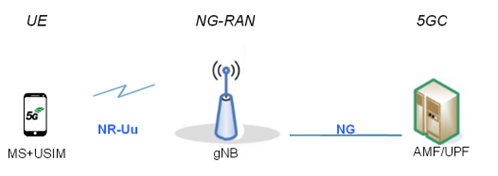
\includegraphics[width=0.8\textwidth, keepaspectratio]{imagenes/estado del arte/5g-fig1.png}
    \caption{Arquitectura general del sistema 5G. Fuente: 3GPP \cite{3gpp_5g_overview}}
    \label{fig:arquitectura5g}
\end{figure}

\par\medskip
\textbf{Nota 1: Como la figura la he cogido de una fuente ¿Se cita así?.}
\par\medskip

\par\medskip
\textbf{Nota 2: Las fuentes están en inglés; cuando se habla de radio coverage, traduzco como cobertura radioeléctrica y radio access dice el chatGPT que se traduce como acceso radio. Me suena un poco raro, pero no se muy bien como traducir eso.}
\par\medskip

Dentro de la NG-RAN, el gNodeB (gNB) actúa como estación base de 5G NR y establece la comunicación radio con el equipo de usuario \cite{3gpp_5g_overview}. Esta comunicación depende de la cobertura proporcionada por la estación base y de las condiciones de propagación de la señal.

El análisis de la cobertura permite determinar las zonas en las que puede establecerse correctamente la comunicación. Para ello, es necesario estudiar la señal recibida en diferentes posiciones y considerar los factores que afectan su propagación.


\section{Modelado}

\subsection{Simulación y modelos}

Para analizar el comportamiento de una red celular antes de su despliegue real, pueden utilizarse simulaciones. Una simulación reproduce la evolución de un sistema real a lo largo del tiempo y permite estudiar su funcionamiento sin realizar experimentos directamente sobre él. Esto resulta útil cuando dichos experimentos son costosos, peligrosos, requieren demasiado tiempo o sus variables de interés son inaccesibles \cite{nist_modeling_simulation}.

Toda simulación requiere un modelo, es decir, una representación simplificada que refleja algunas propiedades del sistema real. Para realizar simulaciones se utilizan principalmente modelos matemáticos, en lugar de modelos físicos u otros medios de representación. Además, las limitaciones y las condiciones de validez del modelo deben tenerse en cuenta al interpretar los resultados \cite{nist_modeling_simulation}.

\par\medskip
\textbf{Nota: Los dos primeros párrafos están sacados de un informe del NIST; supongo que cuenta como fuente de información fiable. El propio NIST cita los libros que utiliza como referencia, pero no los he encontrado online.}
\par\medskip


\subsection{Simulaciones a nivel de enlace y de sistema}

Las simulaciones de comunicaciones inalámbricas pueden realizarse a nivel de enlace o a nivel de sistema:

\begin{itemize}
    \item \textbf{Simulaciones a nivel de enlace:} estudian una comunicación punto a punto entre un transmisor y un receptor. Permiten analizar el comportamiento y las características de un enlace concreto \cite{nvidia_aodt}.

    \item \textbf{Simulaciones a nivel de sistema:} consideran varios enlaces que transmiten y reciben simultáneamente. De esta forma, permiten analizar el comportamiento conjunto de la red y cómo afectan unos enlaces a otros \cite{nvidia_aodt}.
\end{itemize}

Las simulaciones a nivel de enlace se centran, por tanto, en el comportamiento de una comunicación concreta. Por otro lado, las simulaciones a nivel de sistema amplían el análisis a varios transmisores y receptores, permitiendo estudiar su interacción y el rendimiento global del sistema \cite{nvidia_aodt}.


\subsection{Canal de propagación y modelos de canal}

En las comunicaciones inalámbricas, el canal de propagación determina cómo se transmite la señal entre el transmisor y el receptor. Su comportamiento depende de las condiciones del entorno y de la posición de ambos extremos del enlace.

Los modelos de canal se utilizan para representar estas condiciones de propagación mediante distintos escenarios, parámetros y procedimientos, con el objetivo de estimar las características de la señal recibida \cite{etsi138901}.

El 3rd Generation Partnership Project (3GPP) define modelos de canal para distintos escenarios de propagación. Entre ellos se encuentran la microcelda urbana (UMi), la macrocelda urbana (UMa) y los entornos interiores. A su vez, estos modelos distinguen entre condiciones de propagación con línea de visión directa (\textit{Line of Sight}, LOS) y sin línea de visión directa (\textit{Non-Line of Sight}, NLOS) \cite{etsi138901}.


Los escenarios UMi, UMa e interiores se diferencian principalmente por el tipo de entorno, la posición de la estación base y la distancia entre emplazamientos. En UMi, las estaciones base se sitúan por debajo de la altura de los edificios y se consideran entornos como calles, plazas o zonas urbanas abiertas. En UMa, se ubican por encima de los tejados de los edificios circundantes. Por otro lado, los escenarios interiores representan entornos como oficinas y centros comerciales, donde las estaciones base suelen instalarse en paredes o techos a menor altura \cite{etsi138901}.

\par\medskip
\textbf{Nota: Según esta definición, mi escenario sería UMa porque la antena está por encima de los edificios, aunque no llega a los 25 m de altura para UMa según 3GPP. No obstante, como está a decisión del usuario configurar UMi/UMa con ABG y esto es estado del arte, no lo voy a mencionar.}
\par\medskip

Uno de los parámetros principales de estos modelos es la pérdida de propagación, que representa la atenuación experimentada por la señal durante su recorrido. Su cálculo depende del escenario considerado, de la condición LOS o NLOS y de parámetros como la distancia entre el transmisor y el receptor, la frecuencia utilizada y la altura de ambos extremos del enlace \cite{etsi138901}.

Además de la pérdida de propagación, el modelo de 3GPP contempla otros efectos, como el desvanecimiento por sombra, las pérdidas de penetración en edificios y la dispersión temporal y angular de la señal \cite{etsi138901}. La consideración de estos parámetros permite representar con mayor detalle las condiciones de propagación de cada escenario.


\subsection{Modelos de pérdidas de propagación}

\subsubsection{Modelo de pérdidas en el espacio libre}

El modelo de pérdidas en el espacio libre (\textit{Free-Space Path Loss}, FSPL) representa la pérdida de señal producida al propagarse entre un transmisor y un receptor en condiciones de espacio libre. Cuando la distancia entre las antenas es mucho mayor que la longitud de onda, puede calcularse mediante la siguiente expresión \cite{itur_p341}:

\begin{equation}
    L_{\mathrm{bf}}\,(\mathrm{dB})=20\log_{10}\left(\frac{4\pi d}{\lambda}\right)
\end{equation}

donde $d$ es la distancia entre las antenas, expresada en metros, y $\lambda$ es la longitud de onda de la señal, también expresada en metros.

Teniendo en cuenta que $c=\lambda f$, la expresión también puede escribirse como:

\begin{equation}
    L_{\mathrm{bf}}\,(\mathrm{dB})=20\log_{10}\left(\frac{4\pi d f}{c}\right)
\end{equation}

donde $f$ es la frecuencia de la señal, expresada en hercios, y $c$ es la velocidad de propagación de la luz, expresada en metros por segundo.

\par\medskip
\textbf{Nota: Es la de los apuntes de TD, cogí la fuente que estaba puesta en el campus virtual. El resto de fuentes usaba otra versión de L = 32.4 + 20log... que no he usado nunca.}
\par\medskip


\subsubsection{Modelo Alpha-Beta-Gamma}

El modelo Alpha-Beta-Gamma (ABG) es un modelo de pérdidas de propagación a gran escala que expresa las pérdidas en función de la distancia entre el transmisor y el receptor y de la frecuencia de la señal. Este modelo ha sido utilizado en estudios de propagación para redes 5G \cite{abg}. Las pérdidas calculadas mediante el modelo ABG se expresan como:

\begin{equation}
\begin{split}
    PL_{\mathrm{ABG}}\,(\mathrm{dB})={}&10\alpha\log_{10}\left(\frac{d}{1\,\mathrm{m}}\right)
    +\beta \\ &+10\gamma\log_{10}\left(\frac{f}{1\,\mathrm{GHz}}\right)
    +X_{\sigma}^{\mathrm{ABG}}
\end{split}
\end{equation}

donde $d$ es la distancia entre el transmisor y el receptor, expresada en metros; $f$ es la frecuencia de la señal, expresada en GHz; $\alpha$, $\beta$ y $\gamma$ son los coeficientes del modelo; y $X_{\sigma}^{\mathrm{ABG}}$ es una variable aleatoria expresada en dB que representa las variaciones producidas por el desvanecimiento por sombra \cite{abg}.

\par\medskip
\textbf{Nota: Me acabo de dar cuenta (19/07/2026) de que en la fuente (la saqué de  tu TFG, asi que es la misma) pone que esta ecuación solo se cumple cuando d es mayor o igual a 1 m. En el mapa de calor, si ponemos un mapa de 1x1x1 metros con un tamaño de vóxel de 0'1, ninguna medida sería válida porque los 1000 vóxeles del mapa de calor se encuentran a una distancia menor a 1 m.}

\textbf{¿Ignoramos esa condición? No la he añadido a la fórmula por ese mismo motivo. Otra opción es que si se encuentra un receptor a menos de 1m se calculen pérdidas como si estuviese a 1 m (eso lo tenía hecho ya pero con 0.001 m).}

\textbf{En principio, pocas medidas debería haber a esa distancia; solo pasaría en el mapa de calor si el tamaño del vóxel es pequeño y están pegados a la antena.}
\par\medskip

Los parámetros del modelo $\alpha$, $\beta$ y $\gamma$ pueden ajustarse a partir de los datos obtenidos para un escenario determinado \cite{abg}.

\par\medskip
\textbf{Nota: He añadido los modelos FSPL y ABG porque son los modelos de pérdidas que se utilizan posteriormente en el simulador. El CI de interiores me lo he salto porque no está implementado y no se hace nada en interiores.}
\par\medskip


La potencia recibida por los receptores también está condicionada por la forma en que la antena distribuye la energía en el espacio. Por esto, el modelado de su patrón de radiación es otro aspecto fundamental para representar el enlace entre el transmisor y el receptor.


\section{Modelado de antenas}

Las características de una antena determinan cómo se distribuye la energía radiada en el espacio. Esta distribución se representa mediante el patrón de radiación, que muestra cómo varía la ganancia de la antena según la dirección de propagación. Para analizar su comportamiento de forma completa, es necesario disponer de un patrón tridimensional que permita conocer la ganancia alrededor de toda la antena.

Sin embargo, la información proporcionada por los fabricantes se limita a los cortes horizontal y vertical. Estos patrones bidimensionales muestran el comportamiento de la antena en dos planos, pero no permiten conocer directamente los valores correspondientes a las direcciones situadas fuera de ellos. Por este motivo, se han desarrollado diferentes métodos para estimar el patrón tridimensional completo a partir de ambos cortes.

Uno de los procedimientos más sencillos y directos consiste en sumar los valores de los patrones horizontal y vertical expresados en escala logarítmica, normalmente en decibelios, para obtener la ganancia correspondiente a cada dirección. Este método es fácil de implementar y puede proporcionar buenos resultados en antenas omnidireccionales con patrones regulares o simétricos. Sin embargo, en antenas directivas o con patrones más complejos, puede dar lugar a errores importantes, especialmente fuera del lóbulo principal \cite{7268850}.

Gil et al. propusieron un método de interpolación para reconstruir el patrón tridimensional de antenas de estación base a partir de los cortes horizontal y vertical. Su procedimiento combina ambos patrones teniendo en cuenta la dirección que se desea estimar \cite{gil2001}.

Este método utiliza toda la información disponible en los cortes horizontal y vertical, por lo que puede conservar las diferencias existentes entre las distintas partes del patrón vertical. No obstante, no puede reconstruir de forma exacta las características del patrón que no aparecen representadas en dichos cortes. Por este motivo, pueden producirse errores en zonas como los lóbulos secundarios o las direcciones alejadas de los planos principales.

Posteriormente, Vasiliadis et al. presentaron un método de aproximación basado en la combinación ponderada de los dos cortes principales. En lugar de sumar directamente ambos valores, el método asigna un peso diferente a cada corte en función de la distancia angular existente entre la dirección que se desea estimar y los planos horizontal y vertical. De este modo, las direcciones reciben una mayor influencia del plano más cercano \cite{vasiliadis2005}.

Esta combinación ponderada permite reducir el error respecto al método de suma directa. Además, el método presenta buenos resultados tanto para antenas omnidireccionales como para antenas directivas. Sin embargo, su funcionamiento depende de un parámetro k, que controla la forma en que se distribuyen los pesos de los cortes horizontal y vertical. Los autores explican que un valor $k = 2$ minimiza el error de la reconstrucción, aunque también indican que el valor más adecuado puede depender de la directividad y de las características de cada antena \cite{vasiliadis2005}.

Otra limitación del método de Vasiliadis se encuentra en la interpretación del corte vertical. El procedimiento utiliza 360 muestras del patrón horizontal y 180 muestras del patrón vertical \cite{vasiliadis2005}. Si las dos mitades del patrón vertical son simétricas, una de ellas puede utilizarse para representar la otra sin que se produzcan diferencias. Sin embargo, cuando el patrón no es simétrico, la reducción del corte vertical implica la pérdida de la información correspondiente a una de sus mitades.

Además de estos métodos, también es posible reconstruir patrones tridimensionales mediante técnicas de \textit{deep learning}. MathWorks proporciona una implementación que utiliza una red neuronal entrenada para estimar un patrón tridimensional a partir de cortes bidimensionales \cite{mathworks_patternfromai}. La red aprende la relación entre los cortes principales y los patrones tridimensionales reconstruidos a partir de un conjunto de antenas utilizadas durante el entrenamiento.

Este método es más difícil de implementar, ya que requiere una gran cantidad de muestras para entrenar y validar el modelo. Sin embargo, el \textit{deep learning} permite reconstruir patrones más complejos que los métodos anteriores.

El modelado del patrón de radiación permite estimar con mayor precisión la ganancia de la antena en cada dirección y, por tanto, analizar cómo se distribuye la cobertura en el escenario. Este análisis resulta especialmente importante en servicios donde la comunicación debe mantenerse incluso en situaciones de emergencia o en condiciones desfavorables.


\section{Comunicaciones críticas}

Las comunicaciones críticas son aquellas utilizadas por organismos de protección pública y atención ante desastres en situaciones donde la vida humana, los bienes u otros valores de la sociedad están en riesgo, especialmente cuando el tiempo es un factor determinante. Estas comunicaciones deben ser seguras, fiables y estar disponibles cuando se necesiten \cite{itur_m2377}.

Debido a la importancia de estas situaciones, las comunicaciones críticas presentan requisitos más exigentes que otros servicios convencionales. Deben ofrecer baja latencia, alta disponibilidad y fiabilidad, capacidad para gestionar un gran número de usuarios y dispositivos, seguridad y mecanismos de prioridad \cite{etsi122280}.

Además, estos sistemas deben permitir el intercambio de distintos tipos de información. 3GPP utiliza el término MCX para agrupar las aplicaciones críticas, entre las que se incluyen \textit{Mission Critical Push To Talk} (MCPTT), para las comunicaciones de voz; \textit{Mission Critical Video} (MCVideo), para la transmisión de vídeo en tiempo real; y \textit{Mission Critical Data} (MCData), para el intercambio de datos en tiempo real \cite{etsi122280}.

Estos servicios pueden utilizarse en aplicaciones de seguridad pública y en otros ámbitos que requieren una comunicación fiable, como las operaciones marítimas y determinados sectores comerciales \cite{etsi122280}. También permiten realizar comunicaciones entre usuarios individuales y grupos, facilitando el intercambio de información entre los distintos participantes de una operación.

En este contexto, la cobertura es un aspecto especialmente importante. La pérdida de conexión o una calidad insuficiente de la señal puede impedir el intercambio de voz, vídeo o datos en situaciones donde la comunicación resulta necesaria. Por este motivo, el análisis de la propagación permite identificar zonas con problemas de cobertura y estudiar cómo influyen factores como la posición de la antena, el patrón de radiación, la distancia y los obstáculos presentes en el entorno.

Las herramientas de simulación permiten realizar este análisis antes de desplegar o modificar una red. Mediante ellas es posible representar la distribución de la señal en un escenario, evaluar la cobertura en distintas posiciones y localizar las zonas en las que las condiciones de comunicación pueden resultar insuficientes para este tipo de comunicaciones.


\section{V2X y comunicaciones vehiculares}

Las comunicaciones vehiculares permiten intercambiar información entre los vehículos y otros elementos de su entorno. Estas se agrupan bajo el termino V2X, procente de \textit{Vehicle-to-Everything}, y permiten que vehículos, infraestructuras, servidores de aplicaciones y peatones recopilen y compartan información de su entorno para ofrecer servicios relacionados con la seguridad, la eficiencia del tráfico y otras aplicaciones de los sistemas de transporte inteligente \cite{etsi122185}.

3GPP define cuatro tipos de comunicaciones V2X: vehículo a vehículo (\textit{Vehicle-to-Vehicle}, V2V), vehículo a infraestructura (\textit{Vehicle-to-Infrastructure}, V2I), vehículo a red (\textit{Vehicle-to-Network}, V2N) y vehículo a peatón (\textit{Vehicle-to-Pedestrian}, V2P) \cite{etsi122185}.

En las comunicaciones V2V, los vehículos cercanos entre sí intercambian información, como su posición o su movimiento. En V2I, el vehículo se comunica con elementos de la infraestructura, como una unidad situada junto a la carretera, llamada \textit{Roadside Unit} (RSU). En V2N, el vehículo intercambia información con un servidor de aplicaciones a través de la red. Por último, V2P permite la comunicación entre vehículos y usuarios vulnerables, como peatones, mediante los dispositivos asociados a cada uno de ellos \cite{etsi122185}.

El intercambio de esta información permite que los vehículos y el resto de elementos conozcan mejor lo que ocurre en su entorno. A partir de estos datos, se pueden desarrollar aplicaciones como los avisos de colisión, la coordinación entre vehículos o la conducción automatizada. Estas aplicaciones pueden contribuir tanto a mejorar la seguridad vial como a aumentar la eficiencia del tráfico \cite{etsi122185}.

Las comunicaciones V2X tienen requisitos específicos debido al movimiento de los vehículos y a la necesidad de transmitir información en un tiempo reducido. 3GPP establece requisitos relacionados con la latencia, la fiabilidad, el alcance de la comunicación, la densidad de UE y la velocidad de los vehículos. Por ejemplo, para transferir mensajes entre dos UE que soporten aplicaciones V2V o V2P, se establece una latencia máxima de 100 ms, mientras que, en casos como la detección previa a una colisión, la latencia máxima no puede superar los 20 ms \cite{etsi122185}.

Las aplicaciones V2X más avanzadas se pueden agrupar en cuatro categorías: la formación de grupos de vehículos que circulan de manera coordinada, la conducción avanzada, el intercambio de información procedente de sensores y la conducción remota \cite{etsi122186}. Estos casos pueden requerir el envío frecuente de datos y altos niveles de fiabilidad, especialmente cuando la información recibida se utiliza para tomar decisiones sobre el movimiento del vehículo.

En este tipo de comunicaciones, la cobertura y la calidad de la señal son factores fundamentales. El movimiento de los vehículos modifica continuamente la distancia y la dirección respecto a la antena, mientras que los edificios y otros obstáculos pueden introducir pérdidas adicionales. Por ello, el análisis de la propagación permite estudiar cómo varían la potencia recibida y la SNR durante un recorrido e identificar zonas en las que la comunicación vehicular puede no ser viable.


\section{Maximización de la cobertura}

Como se ha explicado anteriormente en este capítulo, cada celda representa el área de cobertura proporcionada por una estación base. La maximización de la cobertura busca ampliar las zonas de la celda en las que los UE pueden acceder a la red y mantener correctamente la comunicación, reduciendo los puntos donde la cobertura es insuficiente.

La maximización de la cobertura no implica simplemente aumentar el alcance de la celda. También es necesario evitar que la señal se extienda más allá de la zona prevista, ya que esto puede aumentar el solapamiento con otras celdas y generar más interferencias. Por este motivo, es necesario mantener un equilibrio entre cobertura y capacidad \cite{etsi132522}.

Para mejorar la cobertura, se pueden optimizar parámetros como la potencia de transmisión, la inclinación de la antena y su orientación horizontal \cite{etsi132522}. Estos parámetros modifican la celda, ya que afectan a la potencia recibida y a las direcciones en las que se concentra la radiación.

El aumento de la potencia de transmisión eleva la potencia recibida por los UE y puede ampliar la zona de la celda en la que la señal supera el nivel necesario para mantener la comunicación. Sin embargo, su valor debe ajustarse para evitar que la cobertura alcance zonas más alejadas de lo previsto.

La inclinación y la orientación horizontal de la antena permiten dirigir el lóbulo principal hacia las zonas donde se desea proporcionar una mayor cobertura. La forma del patrón de radiación determina la ganancia disponible en cada dirección y, por tanto, la distribución espacial de la cobertura.

Uno de los problemas que se busca reducir son los huecos de cobertura. 3GPP define un hueco de cobertura como una zona donde la intensidad de la señal queda por debajo del umbral necesario para que un UE acceda a la red o donde la SINR de la celda servidora y de las celdas vecinas no permite mantener el servicio básico. Estos huecos pueden deberse a obstáculos físicos, a una configuración inadecuada de los parámetros de la antena o a una planificación radioeléctrica insuficiente \cite{etsi132522}.

También pueden aparecer zonas de cobertura débil, en las que la intensidad de la señal, la SNR o la SINR quedan por debajo del nivel necesario para alcanzar el rendimiento previsto. A su vez, puede producirse una cobertura excesiva cuando la señal de una celda alcanza zonas mucho más alejadas de las planificadas \cite{etsi132522}.

Por tanto, la maximización de la cobertura requiere estudiar la distribución de la señal dentro de la celda y ajustar los parámetros de la antena en función del entorno. Las herramientas de simulación permiten comparar distintas configuraciones de potencia, orientación y patrón de radiación, así como localizar huecos y zonas de cobertura débil antes de realizar cambios en una red real.


\section{Herramientas de simulación de canal tridimensional}

El análisis de la cobertura en escenarios tridimensionales puede realizarse mediante herramientas que combinan la representación del entorno con modelos de propagación. Estas plataformas permiten establecer transmisores y receptores dentro de un escenario digital, configurar sus parámetros y estudiar cómo afectan la geometría y los materiales del escenario a la propagación de la señal.

\par\medskip
\textbf{Nota: Me dijiste (José Javier) que debía meter este apartado en el estado del arte y mover el de soluciones alternativas al estado del arte. No obstante, al hacerlo, veo que son equivalentes; he quitado el de soluciones alternativas y lo he metido todo aquí. No sé si el de soluciones alternativas se refería a otra cosa.}
\par\medskip

\subsection{NVIDIA Aerial Omniverse Digital Twin}

NVIDIA Aerial Omniverse Digital Twin (AODT) es una plataforma de gemelo digital para la investigación y el desarrollo de redes 6G. Esta herramienta utiliza NVIDIA Omniverse para representar el entorno tridimensional y tecnologías de \textit{ray tracing} mediante GPU para simular el comportamiento de la propagación radioeléctrica \cite{nvidia_aodt}.

AODT permite realizar simulaciones a nivel de sistema, considerando varios transmisores y receptores que funcionan simultáneamente. La plataforma puede utilizarse tanto en escenarios formados por una única estación base y un bajo número de UE, como en representaciones urbanas con cientos de estaciones base y miles de UE \cite{nvidia_aodt}.

Para modelar la propagación, AODT utiliza un solucionador electromagnético basado en \textit{ray tracing}. Este modelo tiene en cuenta reflexiones, difracciones y efectos de dispersión difusa direccional. También permite definir los patrones de radiación de los elementos de antena, por lo que la ganancia depende de la dirección de propagación \cite{nvidia_aodt}.

AODT combina la simulación del entorno radioeléctrico con simuladores de la red de acceso radio y de los UE. De esta forma, permite estudiar tanto la propagación como el rendimiento a nivel de sistema y probar distintos algoritmos antes de desplegarlos en una red real \cite{nvidia_aodt}.

En la Figura \ref{fig:aodt} se muestra un escenario urbano representado mediante AODT, junto con las trayectorias de propagación simuladas entre el transmisor y el receptor.

\begin{figure}[H]
    \centering
    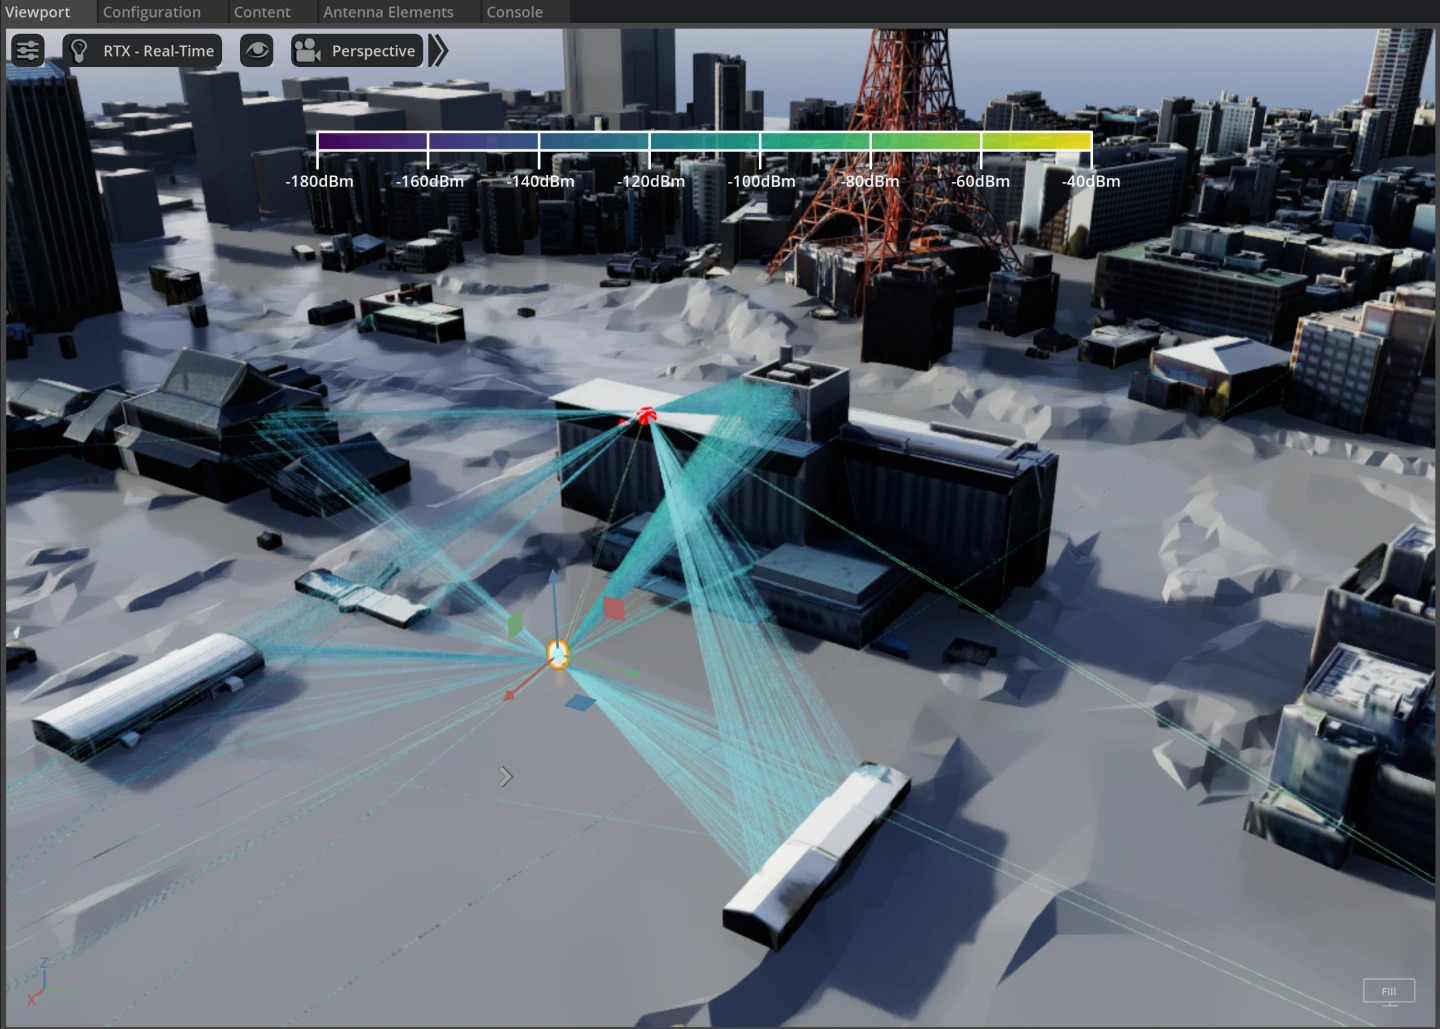
\includegraphics[width=0.9\textwidth]{imagenes/estado del arte/nvidia_aodt.jpg}
    \caption{Simulación de la propagación radioeléctrica mediante NVIDIA AODT. Fuente: NVIDIA \cite{nvidia_aodt}}
    \label{fig:aodt}
\end{figure}


\subsection{Sionna RT}

Sionna RT es una biblioteca de código abierto desarrollada por NVIDIA para el modelado de la propagación radioeléctrica mediante \textit{ray tracing}. Permite representar escenarios tridimensionales y calcular el comportamiento del canal entre transmisores y receptores situados en diferentes posiciones \cite{sionna_rt}.

La herramienta está construida sobre Mitsuba 3, un sistema de renderizado orientado a la simulación del transporte de la luz y al renderizado diferenciable. En Sionna RT, Mitsuba 3 se utiliza para cargar, representar y gestionar la geometría y los materiales de los escenarios tridimensionales \cite{sionna_rt}.

Los escenarios pueden crearse, editarse y exportarse mediante Blender utilizando el complemento Mitsuba-Blender. También es posible generar escenarios a partir de datos de OpenStreetMap mediante complementos específicos de Blender \cite{sionna_rt}.

Una vez cargado el escenario, Sionna RT permite definir transmisores, receptores, patrones de antena y propiedades radioeléctricas de los materiales. A partir de estos elementos, puede calcular los caminos de propagación y obtener parámetros como los coeficientes del canal, los retardos o los ángulos de llegada y salida \cite{sionna_rt}.

En la Figura \ref{fig:sionna_rt} se muestra un escenario urbano de Múnich representado mediante Sionna RT, junto con las trayectorias de propagación calculadas entre un transmisor y un receptor.

\begin{figure}[H]
    \centering
    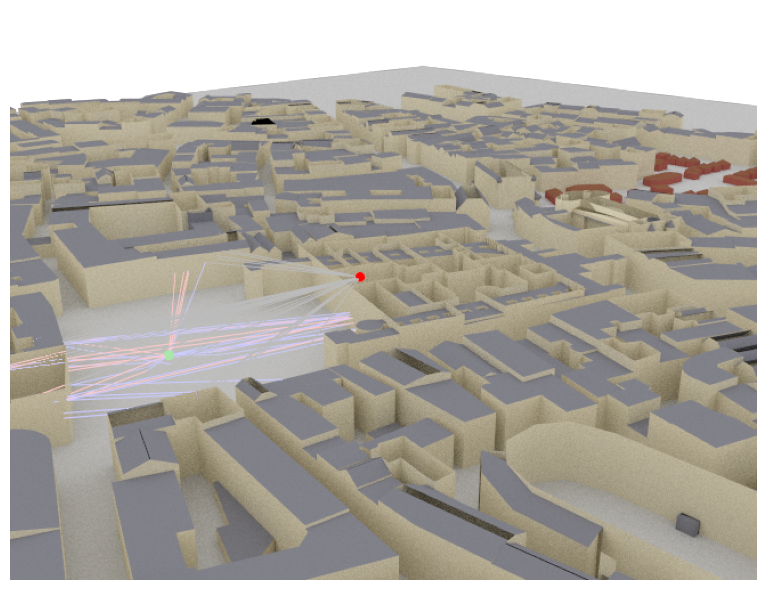
\includegraphics[width=0.9\textwidth]{imagenes/estado del arte/rt_tutorials_Introduction_33_0.png}
    \caption{Escenario urbano y trayectorias de propagación calculadas en Sionna RT. Fuente: NVIDIA \cite{sionna_rt}}
    \label{fig:sionna_rt}
\end{figure}

\subsection{Altair WinProp}

Altair WinProp es una herramienta orientada al análisis de la propagación radioeléctrica y a la planificación de redes inalámbricas. Permite estudiar la cobertura en distintos tipos de escenarios, como entornos urbanos, rurales, industriales e interiores, y dispone de modelos de propagación y funciones de planificación para diferentes tecnologías de comunicación \cite{altair_winprop}.


\subsection{MATLAB}

MATLAB también tiene herramientas para analizar y visualizar la propagación radioeléctrica en escenarios tridimensionales. Mediante \textit{Site Viewer} es posible colocar transmisores y receptores, representar enlaces y generar mapas de cobertura y de SINR tanto en entornos exteriores como interiores \cite{mathworks_rfpropagation}.

Además, MATLAB permite utilizar modelos de \textit{ray tracing} para calcular los caminos seguidos por la señal y estudiar cómo influyen la geometría y los materiales del escenario en la propagación.

En la Figura \ref{fig:matlab_sinr} se muestra un mapa de SINR generado sobre un escenario geográfico. La escala de colores permite identificar las zonas con mejores y peores condiciones de recepción.

\begin{figure}[H]
    \centering
    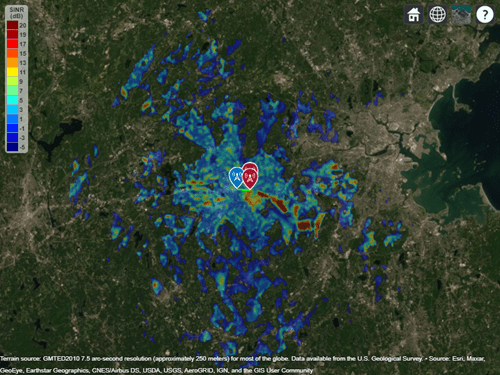
\includegraphics[width=0.8\textwidth]{imagenes/estado del arte/RFPropagationAndVisualizationExample_05.png}
    \caption{Representación de la distribución de la SINR sobre un escenario geográfico mediante MATLAB. Fuente: MathWorks \cite{mathworks_rfpropagation}}
    \label{fig:matlab_sinr}
\end{figure}
\chapter{Diseño del simulador}
\label{chap:diseno_simulador}

En este capítulo se describe el diseño general del simulador desarrollado. Se presenta la arquitectura de la aplicación, el flujo de ejecución y la función de los principales componentes del sistema. Además, se explica cómo se organiza la interfaz de configuración, la escena de simulación, la integración entre Unity y Python, y la exportación de resultados.

\section{Arquitectura general del sistema}

La arquitectura general del simulador se divide en dos grandes bloques: la aplicación desarrollada en Unity y un entorno Python portable integrado. Unity actúa como base de la aplicación, encargándose de la interacción con el usuario, la configuración de la simulación, la construcción del escenario, la visualización de los resultados y la exportación final de datos. Por otra parte, Python se encarga de los cálculos relacionados con el canal de propagación y de la generación automática de gráficas.

En la Figura \ref{fig:arquitectura_general} se muestra el diagrama de componentes del sistema. En la parte superior se representa el bloque de Unity, formado por el menú de configuración, la escena de simulación y el cliente TCP. En la parte inferior se muestra el entorno Python portable integrado, que contiene el servidor TCP, el simulador Python y el generador de gráficas.

\begin{figure}[H]
    \centering
    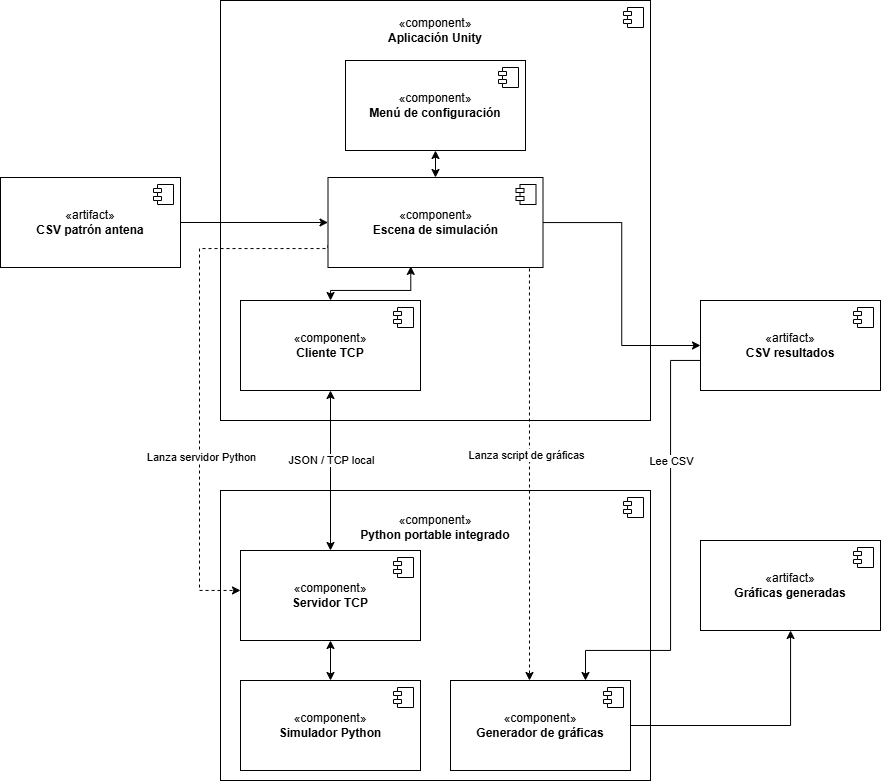
\includegraphics[width=1\textwidth, keepaspectratio]{imagenes/diagramas/Diagrama de componentes.png}
    \caption{Arquitectura general del simulador}
    \label{fig:arquitectura_general}
\end{figure}

Dentro de Unity, el menú de configuración permite introducir los parámetros necesarios para llevar a cabo la simulación, como la potencia de la antena transmisora, la frecuencia, el modelo de propagación o el tamaño de la rejilla que forma el mapa de calor tridimensional. Además, el sistema utiliza como entrada un fichero CSV con información del patrón de radiación de la antena. 

Este fichero contiene características básicas de la antena, junto con los valores del patrón de radiación en los planos horizontal y vertical. Con esta información, Unity reconstruye una aproximación tridimensional del patrón y calcula la ganancia de la antena en función de la dirección entre el transmisor y el punto del escenario deseado.

El entorno Python portable se integra dentro del proyecto para evitar depender de que el usuario final haya instalado Python previamente. Durante la simulación, Unity se comunica con un servidor TCP ejecutado en este entorno, enviando los datos necesarios y recibiendo los resultados calculados. Estos resultados se utilizan para representar la cobertura y generar los archivos de salida.

Con esta arquitectura se busca aprovechar lo mejor de cada entorno. Unity se utiliza para construir el escenario tridimensional, representar la cobertura y permitir que el usuario interactúe en tiempo real, mientras que Python permite reutilizar el simulador de propagación ya existente.

\section{Flujo de ejecución de la aplicación}

El funcionamiento de la aplicación se lleva a cabo a través de dos escenas principales: el menú de configuración y la escena de simulación. En el menú, el usuario ajusta los valores de los parámetros que se utilizarán posteriormente en la simulación. Estos pueden ser tanto técnicos, como la potencia de la antena transmisora, como visuales, de exportación o de rendimiento.

Antes de iniciar la simulación, la aplicación valida los datos introducidos. El usuario no puede avanzar hasta que todos los parámetros sean correctos. Cuando la configuración es válida, los parámetros se guardan y se carga la escena de simulación.

La Figura \ref{fig:flujo_general} muestra el flujo general de la aplicación. El bloque \textit{Ejecutar simulación} representa el proceso completo que se realiza dentro de la escena de simulación. Este proceso se explica en detalle en apartados posteriores de este capítulo.

\begin{figure}[H]
    \centering
    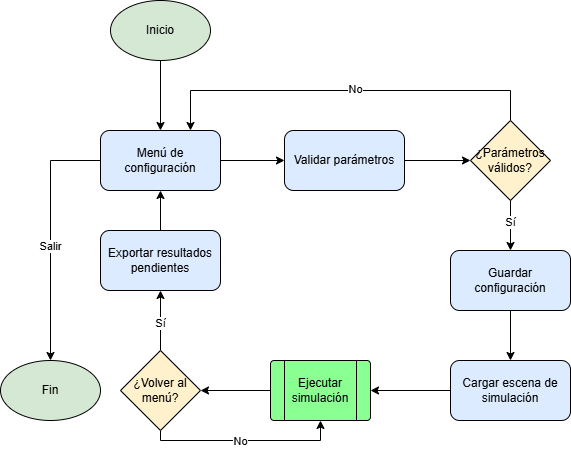
\includegraphics[width=1\textwidth, keepaspectratio]{imagenes/diagramas/Diagrama de flujo general.png}
    \caption{Flujo general de la aplicación}
    \label{fig:flujo_general}
\end{figure}

Durante la simulación, el usuario puede permanecer en la escena observando los resultados o volver al menú de configuración. En caso de volver al menú, la aplicación exporta los resultados pendientes para evitar que se pierda información. Además, desde el menú se puede cerrar la aplicación.

\section{Diseño del menú de configuración}

Una vez se inicia el simulador, el usuario puede elegir entre salir de la aplicación o iniciar la configuración. Desde este menú se ajustan todos los parámetros que se utilizarán posteriormente en la simulación, evitando que estos valores sean fijos o que deban introducirse manualmente a través de un fichero.

El menú está formado por una pantalla principal y cuatro pantallas de configuración. A su vez, estas pantallas se dividen en varias secciones. Esto hace que los parámetros queden organizados por bloques y la configuración sea más clara.

La Figura \ref{fig:diseno_menu} muestra la primera pantalla de configuración, dedicada a la antena y al modelo de propagación. En esta sección se encuentran algunos de los valores principales de la simulación, como la potencia de transmisión, la frecuencia, el ancho de banda, el modelo de pérdidas o el método utilizado para reconstruir el patrón de radiación de la antena.

\begin{figure}[H]
    \centering
    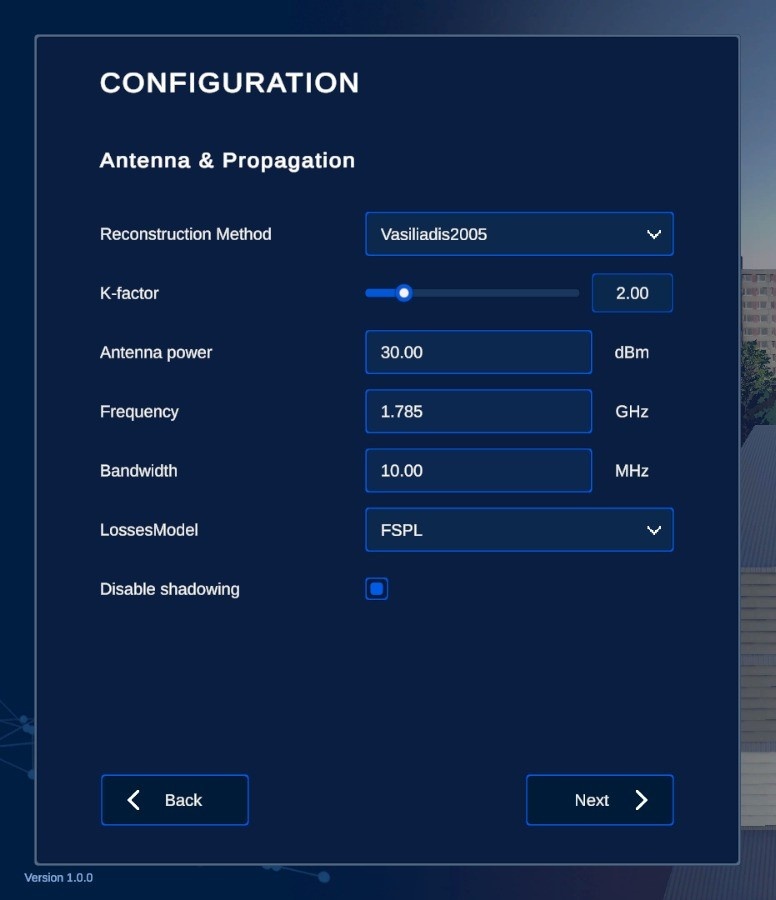
\includegraphics[width=0.75\textwidth, keepaspectratio]{imagenes/diseños/Diseño menu configuracion.jpeg}
    \caption{Diseño del menú de configuración}
    \label{fig:diseno_menu}
\end{figure}

El resto de pantallas siguen la misma idea de organización por bloques. La segunda pantalla permite configurar la rejilla de propagación y los receptores móviles, indicando las dimensiones del mapa de calor, el tamaño de cada vóxel y las ganancias de los receptores. La tercera pantalla agrupa las opciones de visualización y rendimiento, como la transparencia de los vóxeles o el modo de rendimiento de la aplicación. Por último, la cuarta pantalla de resultados y gráficas se utiliza para seleccionar qué gráficas se generarán para cada receptor móvil al finalizar la simulación.

En la pantalla de configuración de la rejilla se muestra también el número total de vóxeles que se generarán con los valores seleccionados. Esto sirve como referencia para que el usuario pueda estimar la carga de la simulación antes de iniciarla, ya que una rejilla más detallada aumenta el número de vóxeles que deben generarse y puede afectar al rendimiento según las características del equipo utilizado.

Antes de cargar la escena de simulación, la aplicación valida los valores introducidos por el usuario. Si algún parámetro no es correcto, no se permite continuar hasta que sea corregido. Una vez validada la configuración, los datos se guardan y se utilizan para inicializar la escena de simulación.

\section{Diseño de la escena de simulación}

La escena de simulación es la parte principal de la aplicación, ya que en ella se encuentran el escenario tridimensional, el patrón de radiación, los mapas de calor y los receptores móviles. Esta escena se carga después de validar la configuración del menú inicial.

La ejecución de la escena sigue el flujo mostrado en la Figura \ref{fig:flujo_ejecucion}. Nada más cargar la escena, el primer paso es cargar la configuración guardada en el menú. A continuación, se reconstruye el patrón de radiación de la antena y se prepara la rejilla de propagación sobre la que se calculará la potencia recibida. Posteriormente, se envían los datos a Python y una vez recibidos los resultados de la rejilla, se representan los mapas de calor. Finalmente, se activan los receptores móviles y, durante la simulación, sus métricas se actualizan y guardan periódicamente.

\begin{figure}[H]
    \centering
    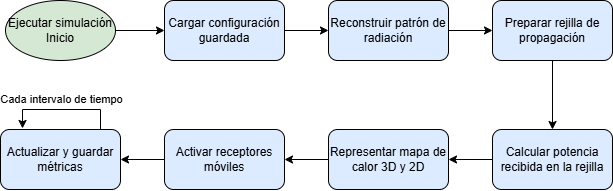
\includegraphics[width=1\textwidth, keepaspectratio]{imagenes/diagramas/Diagrama de flujo - ejecutar simulación.png}
    \caption{Flujo de ejecución de la simulación}
    \label{fig:flujo_ejecucion}
\end{figure}

Para representar la cobertura en el escenario, la aplicación crea una rejilla tridimensional de vóxeles. Un vóxel puede entenderse como el equivalente a un píxel, pero en tres dimensiones: en lugar de representar un punto de una imagen 2D, representa una región del espacio. Para cada vóxel se calcula un valor de potencia recibida y, a partir de ese valor, se colorea la región correspondiente dentro del mapa de calor.

Esta representación permite observar la distribución de potencia dentro de un volumen, pero también tiene una limitación importante. Cuando se muestran muchos vóxeles semitransparentes al mismo tiempo, la visualización puede saturarse y hacer que gran parte del escenario se vea con tonos similares. Por este motivo, se añaden parámetros de transparencia y un umbral de visualización. Las transparencias permiten controlar el peso visual de los vóxeles según su potencia, mientras que el umbral permite ocultar las zonas con menor potencia recibida y centrarse en las regiones más relevantes.

Además del mapa de calor 3D, se añade un minimapa 2D por capas, que permite analizar la misma información en cortes horizontales a distintas alturas. De esta forma, el usuario puede consultar tanto la distribución general de la potencia en el volumen como el comportamiento de una capa concreta. Por defecto, se muestra la capa más próxima a la altura de la antena.

La escena se organiza en varias vistas para evitar mostrar toda la información al mismo tiempo y facilitar la visualización. Las vistas disponibles son las siguientes:

\begin{itemize}
    \item \textbf{Vista del mapa de calor:} muestra la distribución de la potencia recibida en el escenario mediante mapas de calor.
    \item \textbf{Vista del patrón de radiación:} permite observar el patrón de radiación reconstruido de la antena transmisora.
    \item \textbf{Vistas de receptores móviles:} cada receptor móvil tiene una vista propia, en la que la cámara sigue su recorrido y se muestran sus métricas de enlace.
\end{itemize}

Para controlar estas vistas, se utiliza una cámara que cambia de posición según la vista en el modo activo. En las vistas del mapa de calor y del patrón de radiación, la cámara se sitúa alrededor de la antena y puede ajustarse mediante sliders de zoom, rotación y elevación. Estos controles permiten observar los resultados desde distintos ángulos. En las vistas de los receptores móviles, la cámara sigue al receptor seleccionado.

La Figura \ref{fig:vista_heatmap} muestra la vista del mapa de calor dentro de la escena de simulación. En ella se puede ver la distribución de los elementos principales de esta vista, como los controles de cámara, el minimapa, el slider de umbral, los botones de simulación y las opciones de rendimiento.

\begin{figure}[H]
    \centering
    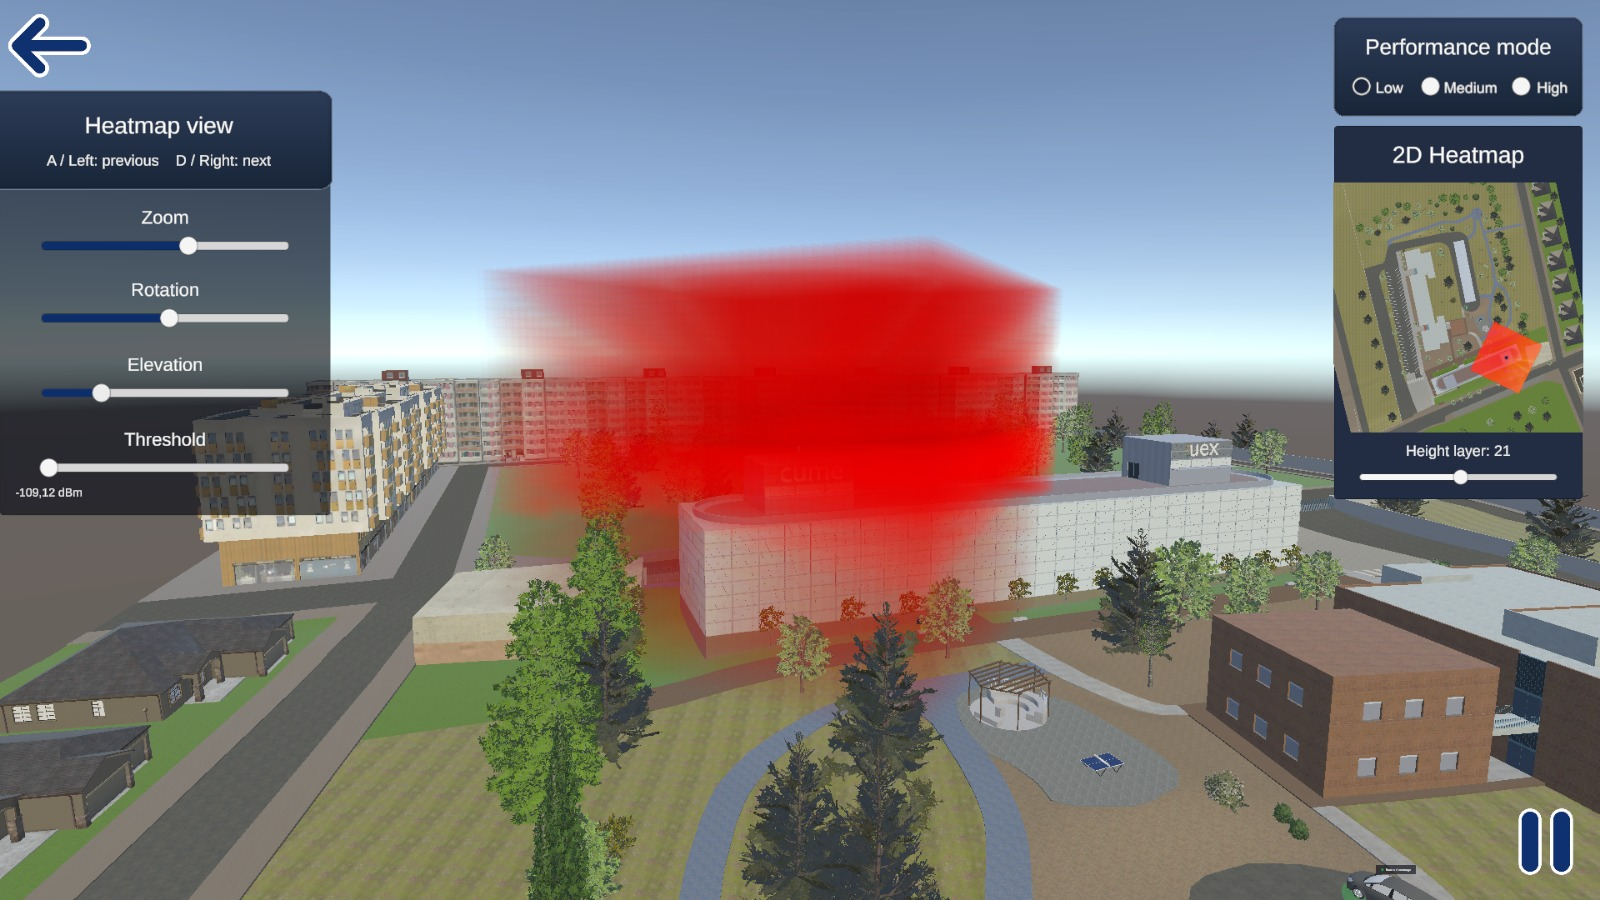
\includegraphics[width=1\textwidth, keepaspectratio]{imagenes/diseños/Diseño heatmapview.jpeg}
    \caption{Vista del mapa de calor}
    \label{fig:vista_heatmap}
\end{figure}

Además, el minimapa puede ampliarse al pulsar sobre él, mostrando la misma información con más detalle, como se observa en la Figura \ref{fig:minimapa_ampliado}. Esta vista ampliada también dispone de una leyenda con los valores mínimo y máximo de potencia recibida, lo que permite interpretar mejor la escala de colores utilizada en el mapa.

\begin{figure}[H]
    \centering
    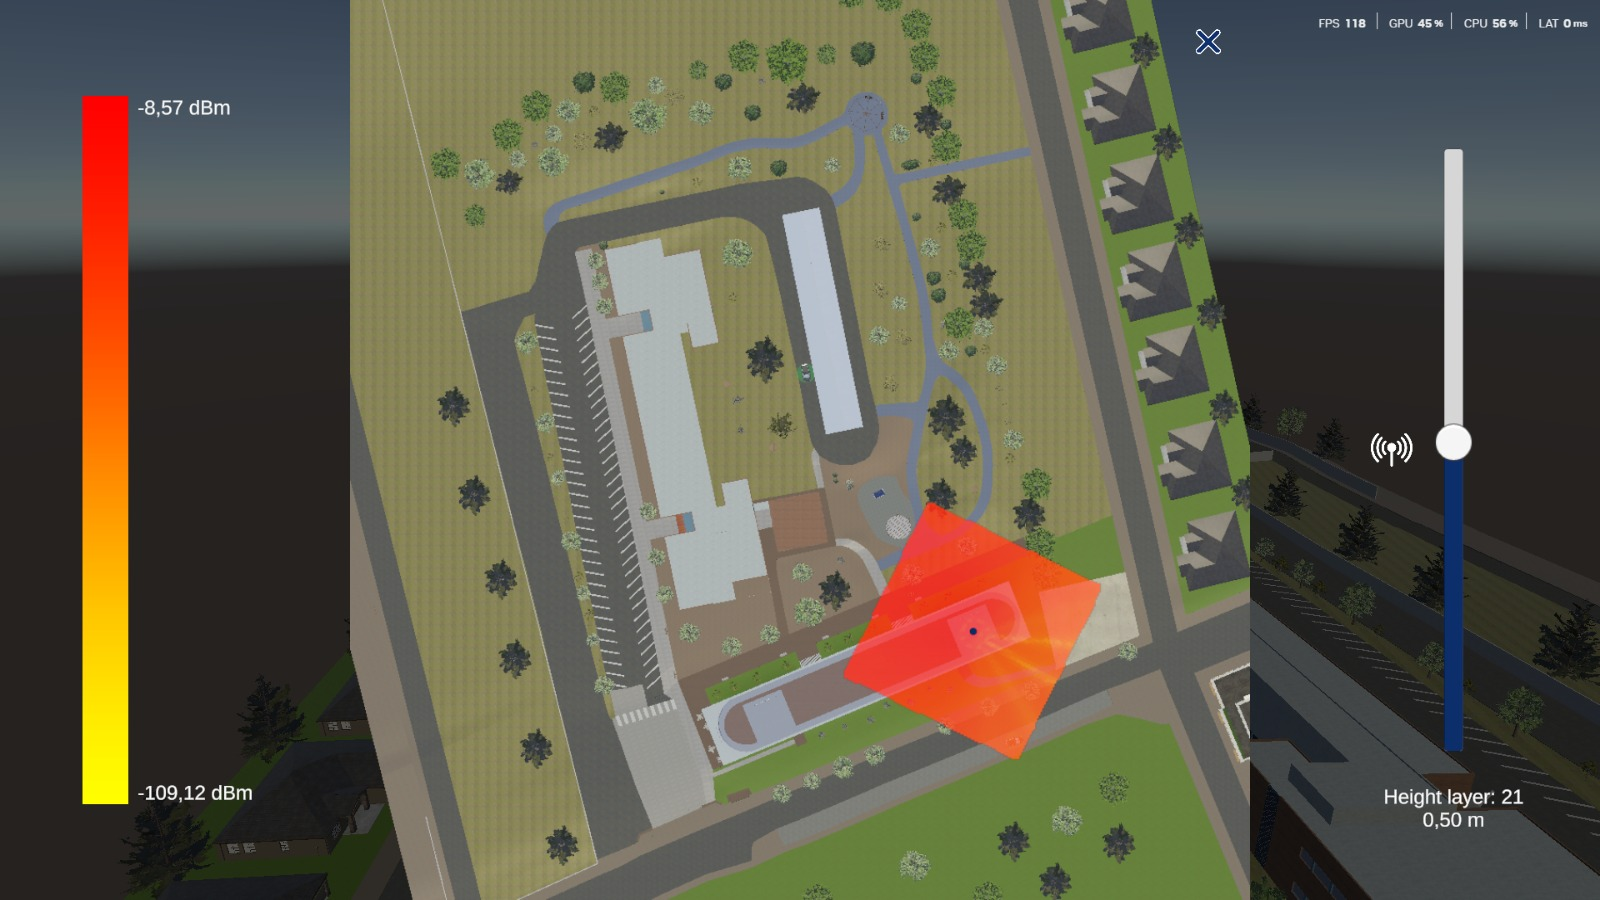
\includegraphics[width=1\textwidth, keepaspectratio]{imagenes/diseños/diseño minimapa ampliado.jpeg}
    \caption{Vista ampliada del minimapa 2D}
    \label{fig:minimapa_ampliado}
\end{figure}

La vista del patrón de radiación permite ver la forma tridimensional del patrón reconstruido, como se muestra en la Figura \ref{fig:vista_patron_radiacion}. Esta vista también incluye una leyenda con la ganancia mínima y máxima en dBi, de forma que el usuario pueda relacionar los colores y la forma del patrón con los valores de ganancia de la antena en cada dirección.

\begin{figure}[H]
    \centering
    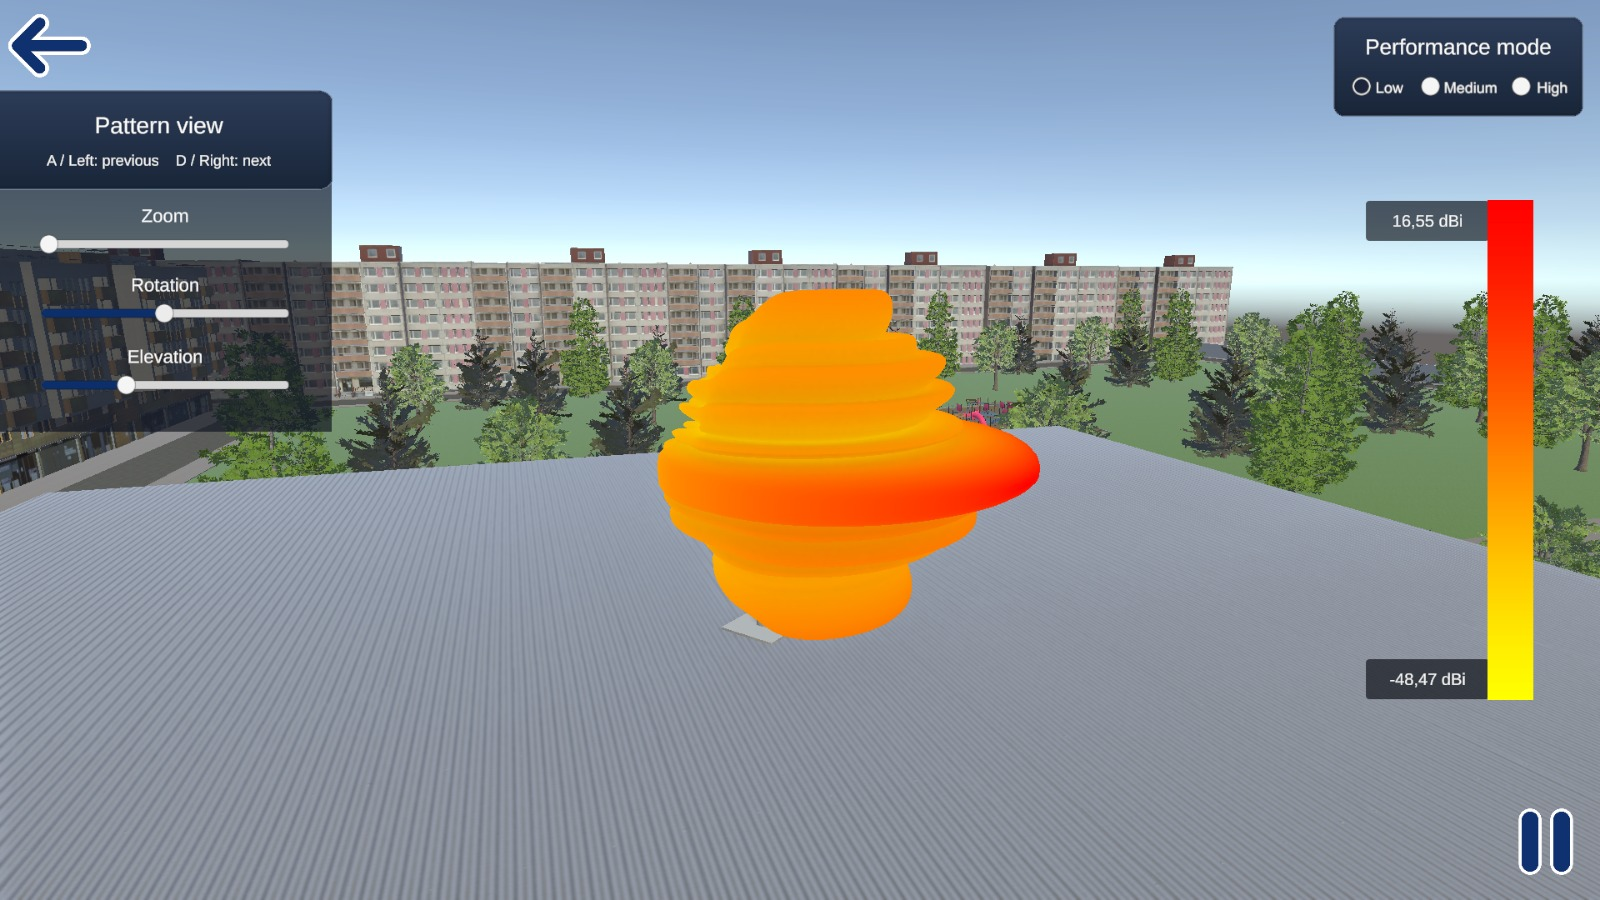
\includegraphics[width=1\textwidth, keepaspectratio]{imagenes/diseños/diseño pattern view.jpeg}
    \caption{Vista del patrón de radiación}
    \label{fig:vista_patron_radiacion}
\end{figure}

Las vistas de receptores móviles permiten seguir el recorrido de cada receptor dentro del escenario y ver sus métricas en tiempo real. En estas vistas, la cámara sigue al receptor seleccionado y se muestra un panel con información como la distancia al transmisor, la potencia recibida, la SNR, las pérdidas del enlace o las colisiones con edificios.

Además de las métricas numéricas, se añade a cada receptor móvil un indicador visual de cobertura. Este indicador muestra un mensaje sobre el receptor con el estado de la cobertura y un círculo de color en el suelo. De esta forma, se puede identificar rápidamente si la cobertura del receptor es excelente, buena, aceptable o insuficiente. En la Figura \ref{fig:vista_receptores} se muestra un ejemplo de vista asociada a un receptor móvil.

\begin{figure}[H]
    \centering
    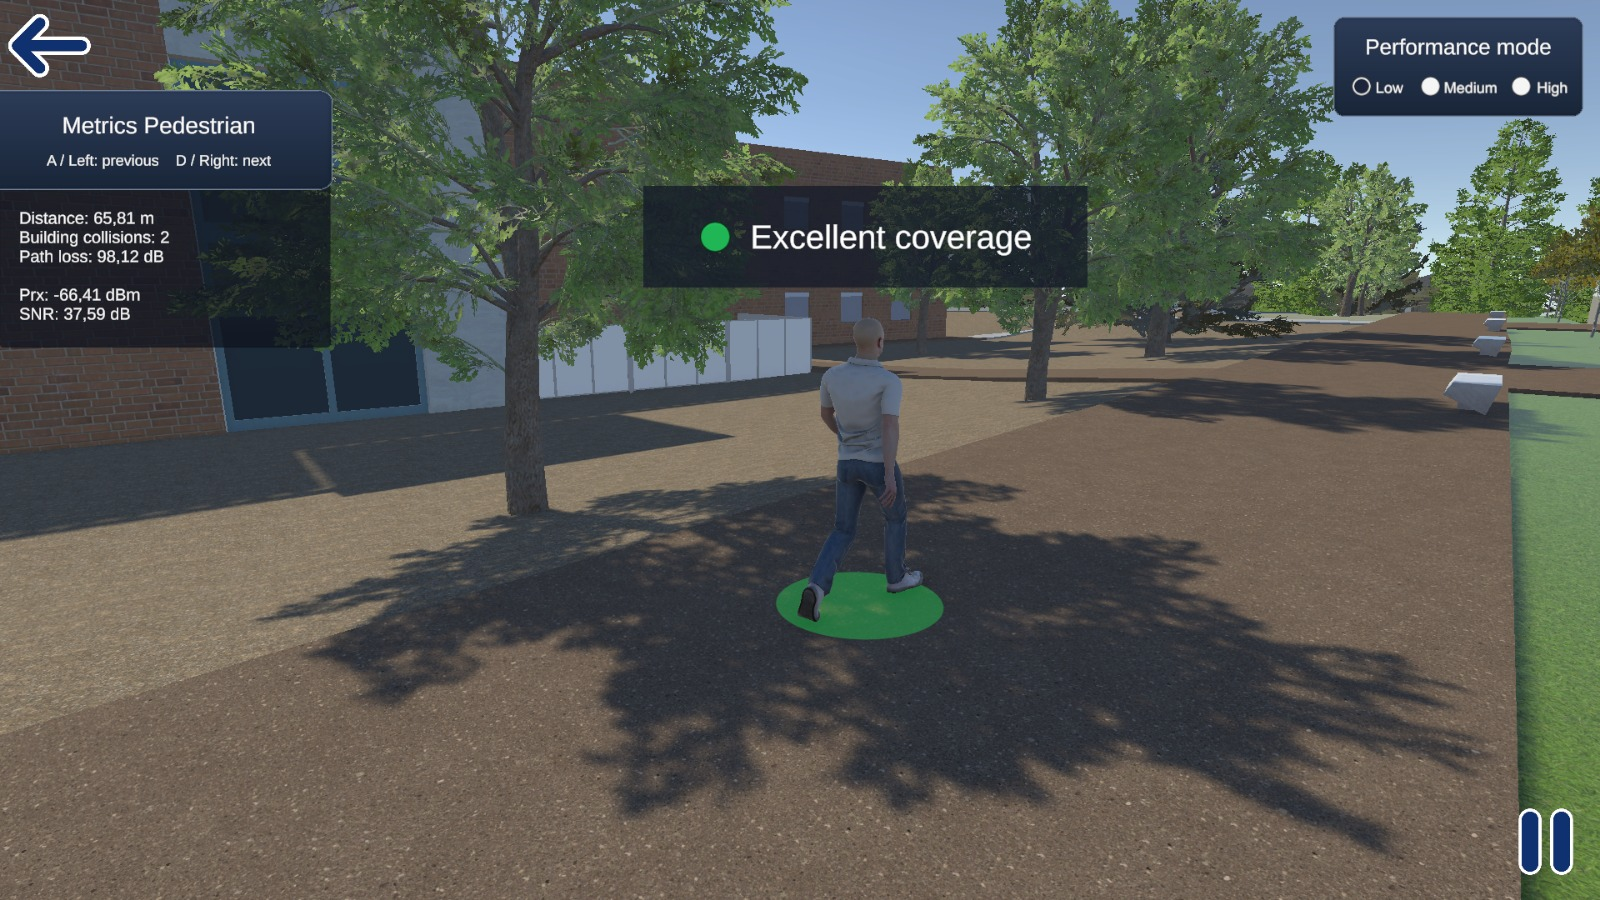
\includegraphics[width=1\textwidth, keepaspectratio]{imagenes/diseños/diseño receptores.jpeg}
    \caption{Vista de un receptor móvil}
    \label{fig:vista_receptores}
\end{figure}

La escena de simulación cuenta también con controles de simulación. En la parte inferior derecha, el botón de pausa permite detener la simulación, cambiando entre el icono de pausa y reanudar según el estado actual. El botón de volver al menú, en la parte superior izquierda, permite salir de la escena de simulación y volver al menú de configuración. Antes de volver, en caso de que queden resultados pendientes, la aplicación exporta los resultados para evitar que se pierdan los datos registrados hasta ese momento.

Por último, en la parte superior derecha se añaden botones de rendimiento. Estos permiten desactivar elementos secundarios del escenario, como vegetación, parque o edificios de fondo. Esta opción es clave para adaptar el simulador a equipos con diferentes prestaciones, ya que la representación del escenario y del mapa de calor puede afectar notablemente al rendimiento.


\section{Integración entre Unity y Python}

La integración entre Unity y Python permite reutilizar el simulador externo ya existente sin tener que reimplementar sus cálculos dentro de Unity. En este proyecto, Unity se encarga de la parte visual e interactiva de la aplicación, además de preparar los datos de la escena, como la rejilla y el patrón de radiación reconstruido. Por otro lado, Python se utiliza para integrar el simulador externo y realizar los cálculos del canal de propagación.

Para facilitar la ejecución de la aplicación, se incluye un entorno Python portable dentro del simulador. Este entorno contiene el intérprete de Python y las librerías necesarias para ejecutar el simulador externo y los scripts auxiliares, evitando que el usuario tenga que instalar Python o configurar dependencias de forma manual.

La comunicación entre ambos entornos se realiza de forma local mediante TCP. Unity actúa como cliente y Python como servidor. Cuando la escena de simulación necesita calcular la potencia recibida en la rejilla o actualizar las métricas de los receptores móviles, Unity prepara una petición y la envía al servidor Python. Una vez procesada, Python devuelve una respuesta con los resultados calculados.

Los mensajes intercambiados entre ambos entornos utilizan formato JSON. Esto permite enviar la información de forma estructurada y facilita la conversión de los datos entre C\# y Python, ya que ambos lenguajes disponen de librerías para serializar y deserializar datos en este formato. De esta forma, Unity puede generar una petición con los parámetros necesarios para la simulación y Python puede devolver una respuesta organizada con los valores obtenidos.


\section{Modelo de datos e intercambio de información}

Para que Unity y Python puedan intercambiar información, los datos se agrupan en Data Transfer Objects (DTO). Estos objetos son clases simples formadas por varios atributos y se utilizan para agrupar los datos que deben enviarse o recibirse en cada petición. Antes de enviar una petición, Unity convierte los DTO a JSON para poder transmitirlos al servidor Python. De la misma forma, cuando recibe una respuesta en JSON, la convierte a DTO para tratar los resultados de forma más sencilla dentro de la aplicación.

La Figura \ref{fig:intercambio_unity_python} muestra el intercambio de información entre Unity y Python para la rejilla de propagación y los receptores móviles.

\begin{figure}[H]
    \centering
    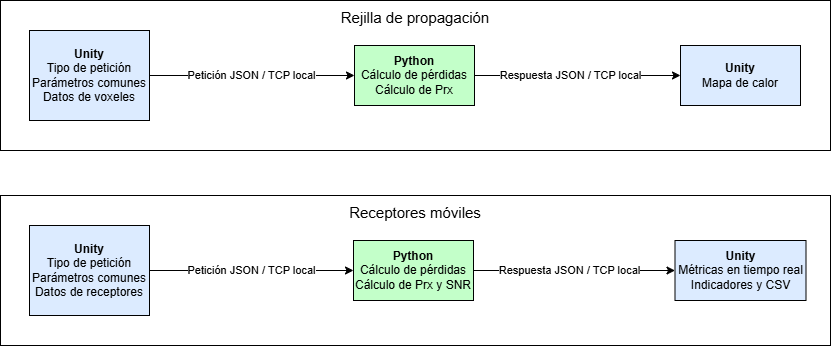
\includegraphics[width=1\textwidth, keepaspectratio]{imagenes/diagramas/Intercambio unity y python.png}
    \caption{Intercambio de información entre Unity y Python}
    \label{fig:intercambio_unity_python}
\end{figure}

En ambos casos, Unity envía una petición a partir de un DTO con parámetros comunes de la simulación, como la frecuencia o la potencia de transmisión, además de la información específica según el cálculo que se quiera realizar.

En el caso de la rejilla de propagación, Unity envía los datos de los vóxeles que forman el mapa de calor. Para cada vóxel se incluye su posición, la ganancia de transmisión correspondiente a esa dirección, el número de colisiones con edificios y la pérdida asociada. Python devuelve para cada punto la distancia al transmisor, las pérdidas del enlace y la potencia recibida. Con estos resultados, Unity colorea los vóxeles para representar el mapa de calor.

En el caso de los receptores móviles, Unity envía la posición actual de cada receptor, la ganancia de recepción y la ganancia de transmisión en la dirección transmisor-receptor. También se envía la información de colisiones y pérdidas asociadas. Python devuelve las métricas calculadas para cada receptor, entre ellas la potencia recibida y la SNR. Estos valores se utilizan para actualizar los paneles de métricas, los indicadores de cobertura y el registro de resultados.

\section{Diseño de la exportación de resultados}

La exportación de resultados se diseña para guardar la información generada durante la simulación y permitir su análisis posterior. Además de mostrar los resultados de forma visual dentro de Unity, el simulador genera archivos externos que pueden consultarse una vez finalizada la ejecución.

Los resultados se guardan dentro de una carpeta \texttt{Results} creada junto a la aplicación. Para cada ejecución se genera una subcarpeta identificada con la fecha y hora de la simulación. De esta forma, cada prueba queda separada del resto sin mezclar archivos generados en ejecuciones distintas.

Durante la simulación, la aplicación registra periódicamente las métricas de cada receptor móvil. Para cada muestra, se almacena el instante de tiempo, la distancia al transmisor, la posición del receptor, la potencia recibida, la SNR, las pérdidas del enlace y el número de colisiones con edificios. Estos datos se guardan posteriormente en archivos CSV, generando un fichero para cada receptor.

Estos CSV guardan todas las muestras obtenidas durante el recorrido. Esto permite reconstruir posteriormente el camino seguido por cada receptor, dibujar otro tipo de gráficas o analizar los datos con otros criterios fuera de la aplicación.

También se exporta un CSV con el patrón de radiación tridimensional reconstruido. Este archivo permite conservar la matriz de ganancias utilizada por el simulador para que pueda revisarse o analizarse fuera de Unity en caso de ser necesario.

Además, se guarda un fichero de configuración de la ejecución, donde se encuentran los parámetros principales utilizados en la simulación. Esto permite reconstruir posteriormente las condiciones de una prueba y comparar los resultados obtenidos con diferentes configuraciones.

A partir de los CSV, la aplicación permite generar gráficas automáticamente. Desde el menú de configuración, el usuario puede seleccionar qué gráficas quiere obtener para cada receptor, como potencia recibida frente a distancia, SNR frente a distancia o SNR frente al tiempo. Al finalizar la simulación, se utiliza el entorno Python integrado para generar estas gráficas a partir de los datos exportados.

Las gráficas frente a la distancia no se deben interpretar como una relación única entre distancia y cobertura, ya que en un escenario tridimensional existen muchos puntos distintos a una misma distancia del transmisor. La potencia recibida y la SNR también dependen de la dirección respecto al patrón de radiación, la altura, los obstáculos atravesados y el recorrido seguido por el receptor. Aun así, estas gráficas son útiles para comparar distintas configuraciones de simulación, patrones de antena o modelos de propagación bajo un mismo recorrido.

La exportación también se tiene en cuenta al volver al menú de configuración. Si el usuario sale de la escena de simulación y existen resultados pendientes, la aplicación los exporta antes de cargar de nuevo el menú.
\chapter{Desarrollo e implementación}
\label{chap:desarrollo}

En este capítulo se describe el desarrollo e implementación del simulador a partir del diseño presentado anteriormente. Se explica cómo se configuró el proyecto en Unity, cómo se construyó el escenario tridimensional y cómo se implementaron los elementos principales de la simulación: la reconstrucción del patrón de radiación, la generación de la rejilla de vóxeles, el cálculo de métricas mediante Python, la representación de los mapas de calor, el seguimiento de receptores móviles, la exportación de resultados y las optimizaciones de rendimiento.

\section{Configuración inicial del proyecto Unity}

La primera parte del desarrollo consiste en preparar la base sobre la que se desarrolla el simulador. Antes de implementar los cálculos de cobertura o la visualización de resultados, se debe organizar el proyecto, crear las escenas principales y preparar todos los elementos involucrados en la simulación.

El proyecto se divide en dos escenas principales: una para el menú de configuración y otra para la simulación, siguiendo la estructura definida en el capítulo anterior. Esta separación permite organizar, por un lado, los elementos de la interfaz inicial y, por otro, los componentes propios de la escena de simulación.

También se organiza la estructura de carpetas del proyecto. Los scripts se agrupan según su función en tres grupos principales: scripts del menú, scripts de configuración de la simulación y scripts de simulación. A su vez, los scripts de simulación se dividen en varios subgrupos: patrón de radiación, receptores móviles, rendimiento, rejilla de propagación, comunicación con Python y visualización.

Además, se crean carpetas específicas para otros recursos utilizados por la aplicación. Los modelos 3D se organizan en una carpeta específica, junto con carpetas separadas para prefabs, materiales, shaders, sprites y render textures. Esta separación facilita la localización de cada tipo de recurso y evita mezclar todos los recursos en una misma carpeta.

Por otro lado, se utiliza la carpeta \texttt{StreamingAssets} para guardar los recursos que deben estar disponibles durante la ejecución, como el simulador externo, el entorno Python portable, sus librerías y los archivos de entrada. Esta carpeta se mantiene tanto durante el desarrollo como después de compilar la aplicación, por lo que Unity puede acceder a estos recursos en tiempo de ejecución sin depender de rutas externas al proyecto.

También se utiliza una clase de configuración común para conservar los valores introducidos por el usuario en el menú. Cuando la configuración es válida y se carga la escena de simulación, estos valores se leen y se aplican a los componentes correspondientes. Esto permite compartir parámetros entre ambas escenas del simulador.

Con esta base preparada, el siguiente paso es la preparación del escenario donde se lleva a cabo la simulación.

\section{Desarrollo del escenario tridimensional}

A la hora de crear el escenario 3D sobre el que se lleva a cabo la simulación, en lugar de realizarse sobre un entorno urbano genérico, se decide llevar a cabo una recreación tridimensional del Centro Universitario de Mérida. Esta elección permite trabajar sobre un escenario realista aprovechando que el desarrollo del TFG se realiza en este mismo centro.

Dentro de esta recreación, la antena transmisora se sitúa en la misma zona en la que se encuentra una antena real del centro universitario. De esta forma, el escenario no solo sirve como un entorno visual, sino que también permite analizar la cobertura tomando como referencia una ubicación realista dentro del centro.

Para recrear las proporciones del Centro Universitario de Mérida, se utiliza Google Earth como referencia principal \cite{googleearth}. A partir de la vista aérea se obtienen las proporciones en planta de los edificios, carreteras, zonas verdes y el resto de elementos principales. Para estimar las alturas, se toman como referencia los valores de elevación respecto al nivel del mar proporcionados por Google Earth, calculando la diferencia entre la altura del suelo y la altura aproximada de los techos.

Esta forma de trabajar tiene algunas limitaciones. Las alturas obtenidas desde Google Earth se muestran en metros enteros, por lo que las medidas no pueden ser consideradas exactas. Además, el terreno del campus no es completamente plano, lo que introduce pequeñas diferencias de altura entre distintas zonas del mismo. Por este motivo, la topología del escenario no pretende ser una reproducción exacta, sino una aproximación lo suficientemente fiel como para utilizarse a modo de base para la simulación.

El escenario se modela íntegramente en Blender. En primer lugar, se crea un plano base para representar el terreno del campus. Este plano se divide en distintos cuadrados, ajustando la altura de cada zona según los valores de elevación obtenidos a partir de Google Earth. De esta forma, el terreno no queda completamente plano, sino que reproduce de forma aproximada los cambios de altura del entorno real.

Una vez definido el terreno base, se construyen los edificios principales del centro. Para ello, se modelan sus volúmenes partiendo de la vista en planta y de las alturas obtenidas mediante Google Earth. Posteriormente, se añaden el resto de elementos como ventanas, puertas, salientes y otros detalles visibles desde el exterior. Una vez terminados los edificios, se añaden el resto de elementos del campus, como aparcamientos, bancos, vallas o caminos.

Además de la información obtenida de Google Earth, se realizan fotografías del campus desde distintos puntos de vista. Estas imágenes no sirven como base para realizar el modelo, pero sí como apoyo para cuadrar detalles que no se aprecian correctamente desde la vista aérea, como la altura de las ventanas o puertas, las zonas entre edificios o los detalles de algunos elementos del escenario. 

En el caso de las alturas de ventanas o puertas, se realizó una aproximación realizando una regla de tres sobre las fotografías y aplicando las proporciones obtenidas sobre el modelo 3D. Este método no es del todo exacto, pues introduce un error debido a la perspectiva de las imágenes, pero es una solución razonable al no disponer de planos exteriores detallados del centro.

Tras finalizar la creación del modelo, se crearon versiones simplificadas de cada edificio usando un estilo low poly. Esto consiste en crear una réplica del edificio con una geometría más simple. En este proyecto, estas versiones se utilizan para las colisiones y la detección de obstáculos, ya que no es necesario que tengan todos los detalles visuales del modelo original. Esto es importante porque reduce la complejidad de las comprobaciones de colisión y ayuda a optimizar el simulador.

Para mejorar el aspecto visual del modelo, se utilizan texturas externas procedentes de webs como ambientCG \cite{ambientcg} y Poly Haven \cite{polyhaven}. Además, los edificios y la vegetación que rodean el campus se añaden mediante assets descargados de BlenderKit \cite{blendkit}. Estos elementos se utilizan únicamente para completar el fondo visual de la escena, por lo que no intervienen en los cálculos de propagación ni en la detección de obstáculos.

En las Figuras \ref{fig:comparacion1} y \ref{fig:comparacion2} se muestran los resultados del modelado, comparando imágenes reales del Centro Universitario de Mérida con su versión recreada en Blender.

\begin{figure}[H]
    \centering
    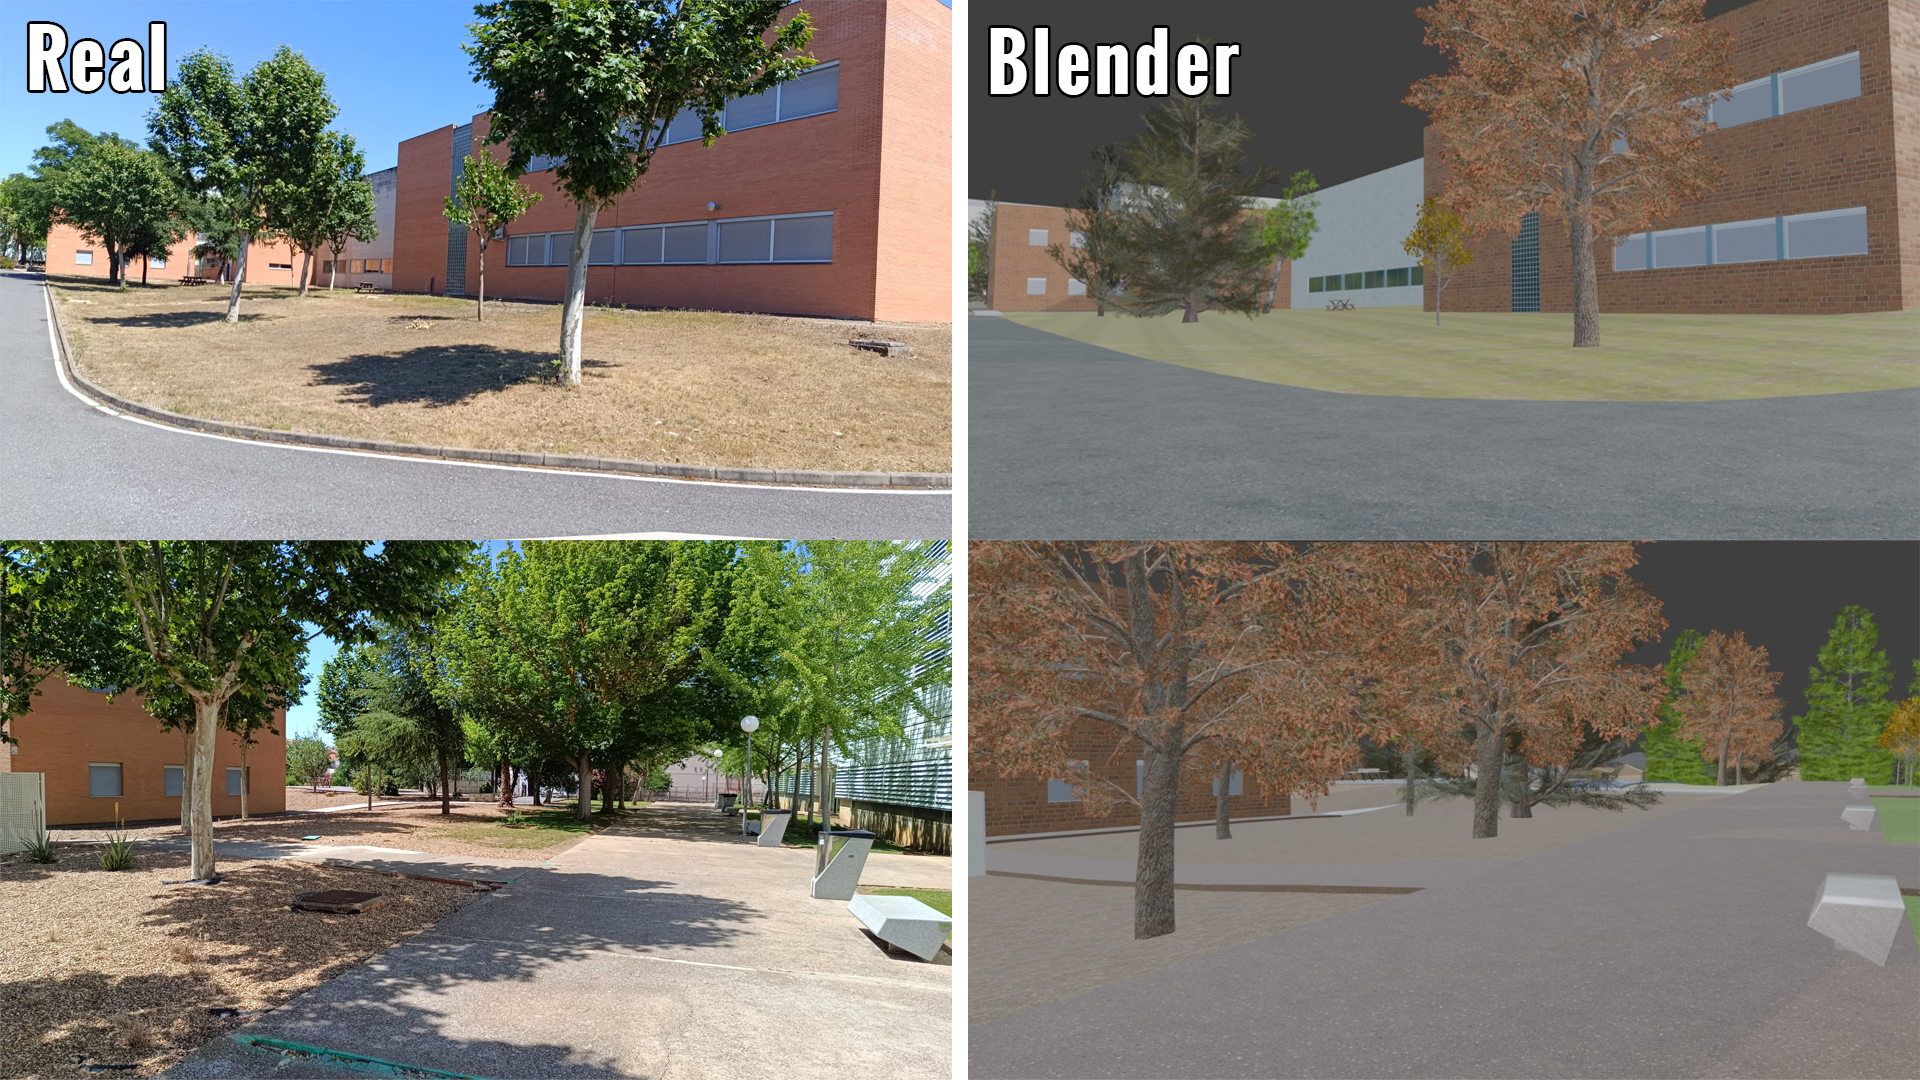
\includegraphics[width=1\textwidth, keepaspectratio]{imagenes/modelo/Comparacion1.png}
    \caption{Primera comparación entre el campus real y el modelo 3D recreado}
    \label{fig:comparacion1}
\end{figure}

\begin{figure}[H]
    \centering
    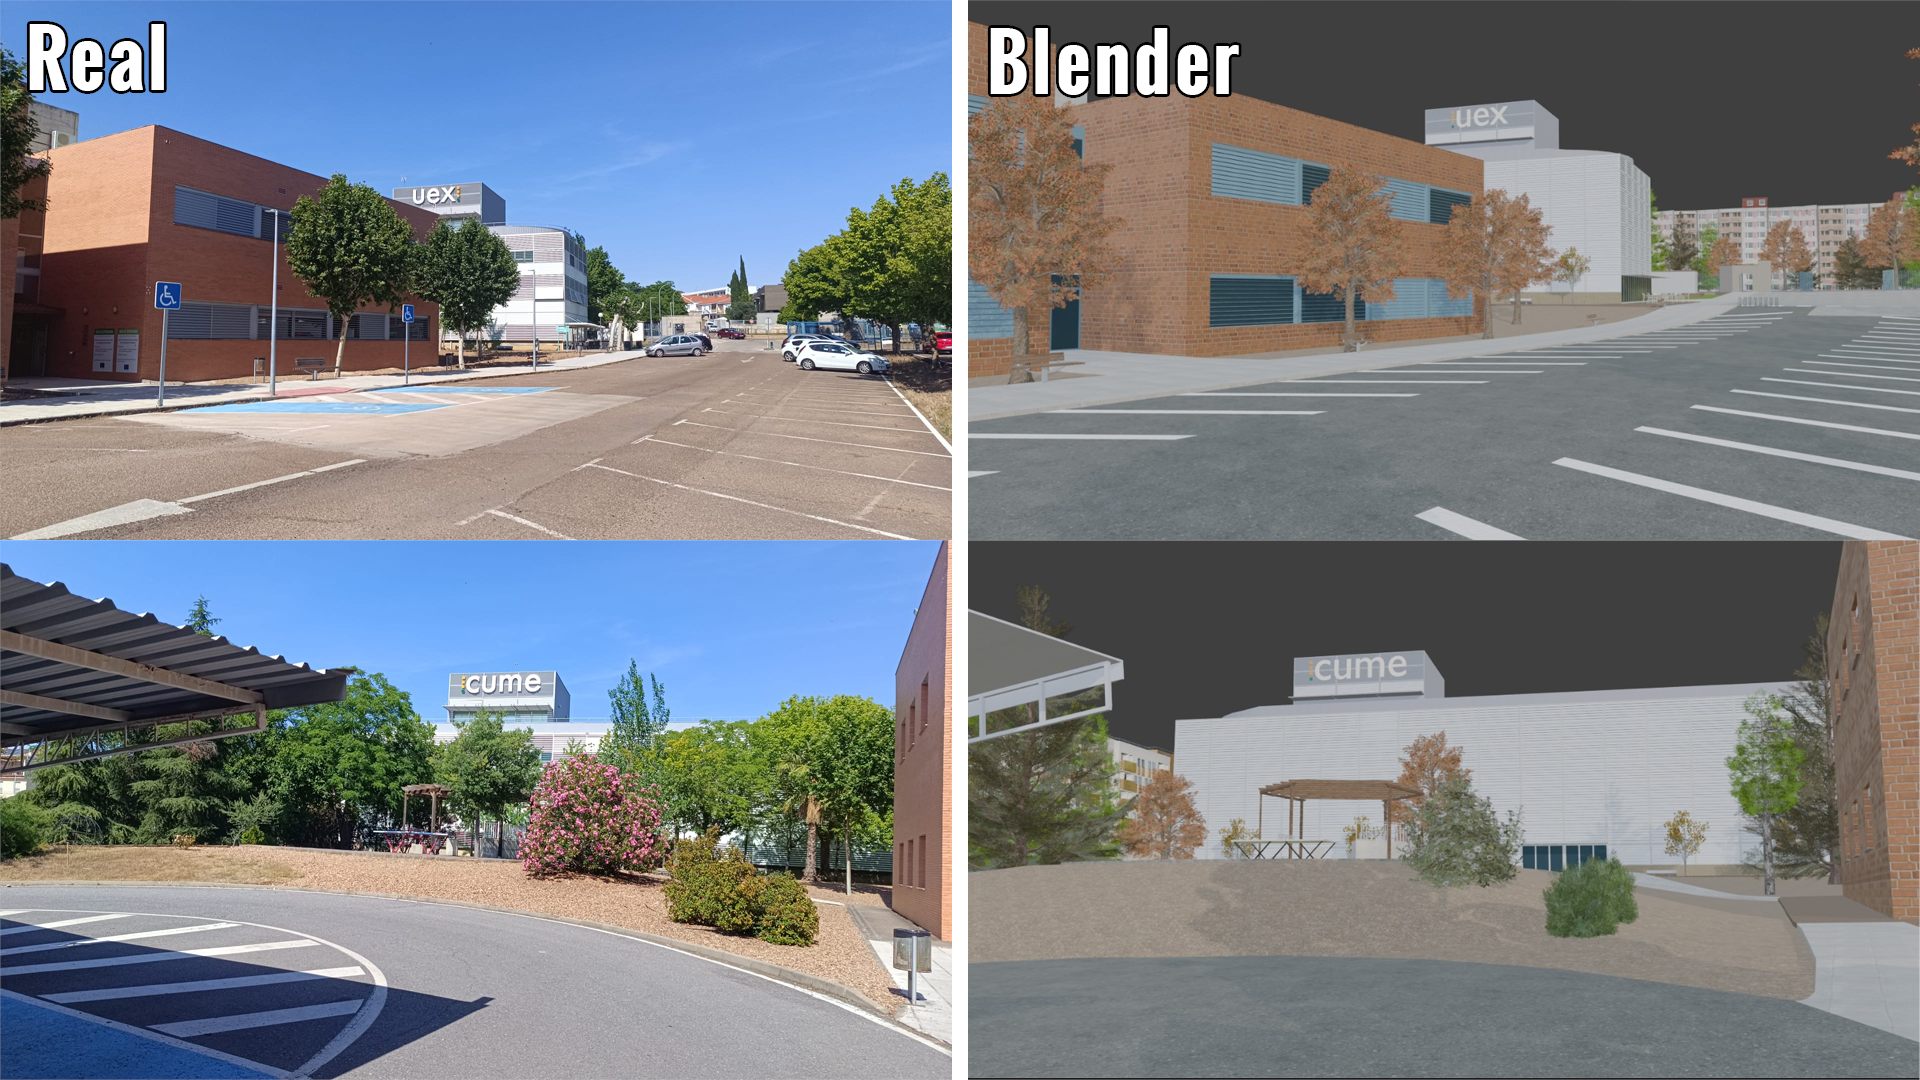
\includegraphics[width=1\textwidth, keepaspectratio]{imagenes/modelo/Comparacion2.png}
    \caption{Segunda comparación entre el campus real y el modelo 3D recreado}
    \label{fig:comparacion2}
\end{figure}

Una vez finalizado el modelo, se importa en Unity, donde se añaden la iluminación, las sombras y el cielo de la escena. El resultado final del escenario integrado en Unity se muestra en la Figura \ref{fig:escenario_unity}.

\begin{figure}[H]
    \centering
    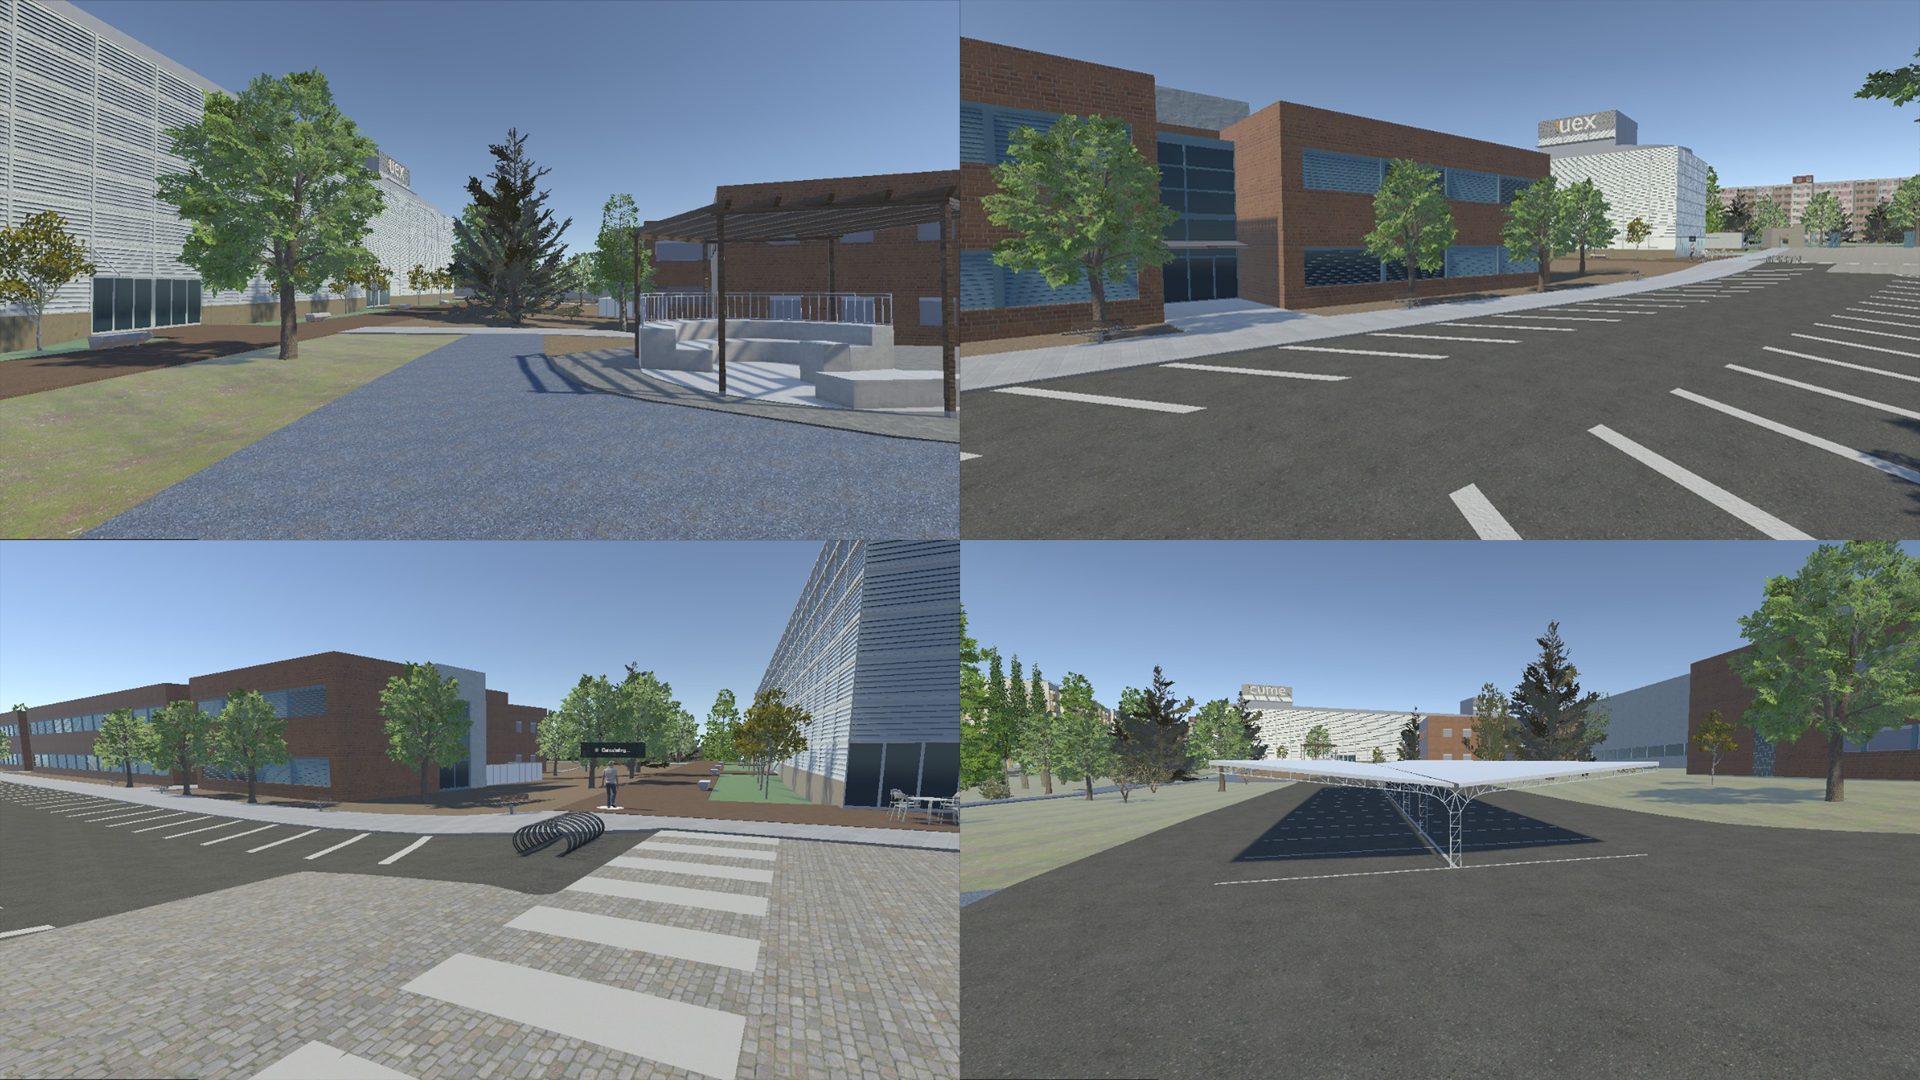
\includegraphics[width=1\textwidth, keepaspectratio]{imagenes/modelo/collage.png}
    \caption{Resultado final del escenario integrado en Unity}
    \label{fig:escenario_unity}
\end{figure}


\section{Reconstrucción del patrón de radiación de la antena}

Una vez preparado el escenario en Unity, el siguiente paso consiste en definir el comportamiento de la antena transmisora dentro de la simulación. Para ello, se implementa la reconstrucción del patrón de radiación.

En este proyecto se implementan tres modos: un patrón omnidireccional, el método de Gil y el método de Vasiliadis. El método utilizado se selecciona desde el menú de configuración, lo que permite estudiar y comparar distintos patrones de radiación.

En el caso de los métodos de Gil y Vasiliadis, la reconstrucción parte de un fichero CSV que contiene los cortes horizontal y vertical del patrón, junto con datos básicos de la antena. A partir de estos cortes, el simulador genera una matriz de ganancia tridimensional según dos ángulos: el ángulo vertical, entre 0 y 180 grados, y el ángulo horizontal o azimut, entre 0 y 359 grados.

Antes de aplicar los métodos de reconstrucción, se deben adaptar los datos del CSV de entrada. El fichero original contiene el corte vertical en función de la elevación, donde la dirección principal del patrón se encuentra a una elevación de $0^\circ$. Sin embargo, la matriz utilizada internamente en Unity representa el ángulo vertical de otra forma: $0^\circ$ corresponde a la dirección superior, $90^\circ$ al plano horizontal de la antena y $180^\circ$ a la dirección inferior.

Por esta diferencia entre referencias, el corte vertical se desplaza $90^\circ$ antes de reconstruir el patrón tridimensional. De esta forma, el máximo del corte vertical queda alineado con el plano del corte horizontal. Además, ese máximo queda centrado dentro del rango vertical utilizado por la matriz, entre $0^\circ$ y $180^\circ$, dejando una parte del patrón por encima y otra por debajo de la dirección principal.

Esta adaptación es importante para aplicar correctamente los métodos de reconstrucción. En el método de Vasiliadis, el corte vertical se utiliza dentro del rango de $0^\circ$ a $180^\circ$, mientras que en el método de Gil el patrón se separa en dos hemisferios respecto al plano horizontal. Si no se realizara este desplazamiento, el lóbulo principal quedaría en la parte superior de la matriz y los cortes horizontal y vertical no estarían alineados correctamente. Esta forma de ajustar los cortes coincide también con el criterio utilizado en las funciones de reconstrucción de patrones en MATLAB.

\par\medskip
\textbf{Nota: No puedo justificar esto último de ninguna forma, en la documentación de matlab no aparece pero, cuando usas la función en matlab, te obliga a tener el máximo en 90º. No sé si está bien dejarlo así o mejor quitar la última frase ya que no tengo referencia en la que apoyarme.}
\par\medskip

Después de alinear los cortes, se preparan los valores que se utilizarán en la reconstrucción. El CSV proporciona el patrón de radiación como atenuaciones en dB, donde la dirección principal del patrón corresponde a la menor atenuación, es decir, 0 dB. A partir de estos valores se obtiene la atenuación relativa de cada dirección.

A continuación, las atenuaciones relativas en dB se convierten a escala lineal. Con esta conversión, la dirección principal del patrón tiene valor 1 y el resto de direcciones quedan normalizadas entre 0 y 1 según su atenuación. Esta representación lineal normalizada es la que utilizan los métodos de reconstrucción para combinar los cortes. Una vez reconstruida la matriz tridimensional, los valores obtenidos se convierten de nuevo a dB relativos y se suma la ganancia máxima indicada en el CSV para obtener la ganancia absoluta en dBi de cada dirección.

El método de Gil utiliza los cortes horizontal y vertical para estimar la ganancia en cada dirección del espacio. Para ello, se separa el comportamiento del plano vertical en una parte frontal y una parte trasera, y se combinan los valores disponibles según la dirección que se quiere reconstruir. De esta forma, se obtiene una aproximación de la ganancia para cada combinación de ángulo vertical y ángulo horizontal.

El método de Vasiliadis también parte de los cortes horizontal y vertical, pero combina ambos valores mediante una ponderación controlada por un factor $k$ configurable. En la aplicación, este factor se puede modificar desde el menú de configuración cuando se selecciona este método. Esto permite ajustar cómo influyen los cortes horizontal y vertical en la reconstrucción del patrón.

Además de estos dos métodos, se implementa un patrón omnidireccional. En este caso, el patrón no se obtiene desde el CSV, sino que se genera mediante una función basada en el seno del ángulo vertical. De esta forma, la ganancia es constante en el plano horizontal y varía únicamente según el ángulo vertical. La ganancia máxima del patrón omnidireccional puede configurarse desde el menú inicial.

En el caso del patrón omnidireccional, la función senoidal utilizada hace que la ganancia sea 0 en los polos. Para evitar problemas al convertir este valor a escala logarítmica, se utiliza un límite mínimo de $10^{-12}$, equivalente a -120 dB. Este valor se mantiene en los cálculos internos, pero no se utiliza directamente para colorear el patrón de radiación. En la visualización, se limita el rango a 50 dB por debajo de la ganancia máxima, facilitando que las diferencias de ganancia sean más visibles en la representación tridimensional del patrón.

Al finalizar la reconstrucción, se generan varias matrices de ganancia. La matriz principal es la de ganancia absoluta en dBi, ya que se utiliza para calcular la ganancia transmisor-receptor, representar el color del patrón y exportar el patrón reconstruido. Además, se conserva una matriz en escala lineal normalizada, utilizada para la construcción del patrón omnidireccional tridimensional, y una matriz de ganancia relativa en dB, utilizada para pruebas internas de la aplicación.

Una vez generada la matriz de ganancia, el patrón se representa en Unity mediante un objeto tridimensional. Esta visualización permite comprobar la forma obtenida con cada método y comparar las diferencias entre el patrón omnidireccional, el método de Gil y el método de Vasiliadis. En la Figura \ref{fig:comparacion_patrones_radiacion} se muestran los tres patrones disponibles en la aplicación.

\begin{figure}[H]
    \centering
    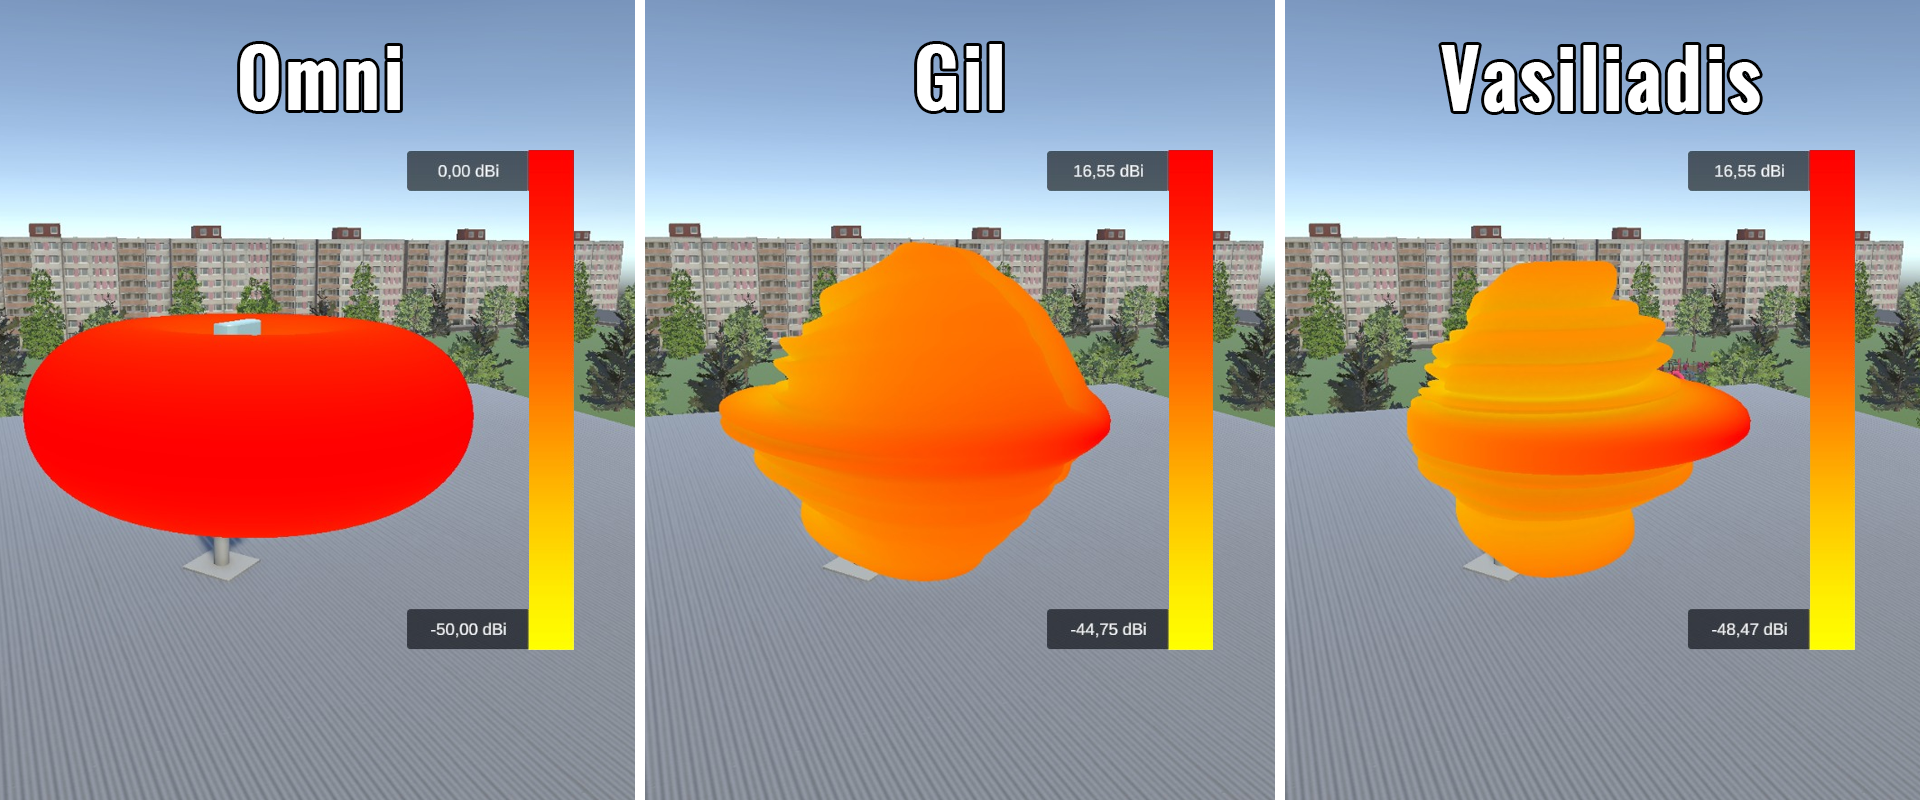
\includegraphics[width=1\textwidth, keepaspectratio]{imagenes/patron de radiacion.png}
    \caption{Comparación de los patrones de radiación implementados}
    \label{fig:comparacion_patrones_radiacion}
\end{figure}


\section{Generación de la rejilla de propagación}

Una vez reconstruido el patrón de radiación, se genera la rejilla de propagación sobre la que se calcula la potencia recibida. Esta rejilla se construye a partir de los parámetros definidos previamente en el menú de configuración: las dimensiones en los ejes X, Y y Z y el tamaño de cada vóxel.

A partir de estos valores, el simulador calcula el número de vóxeles necesario en cada eje. Además, al realizar dicho cálculo, se divide el tamaño de la rejilla entre el tamaño del vóxel y el resultado se redondea hacia arriba. De esta forma, se garantiza que el volumen configurado quede cubierto por completo, aunque las dimensiones elegidas no sean múltiplos exactos del tamaño del vóxel.

La generación de la rejilla se realiza usando la antena transmisora como referencia. Primero, se obtiene la esquina mínima del volumen en coordenadas locales de la antena, y desde esa posición se recorren los tres ejes de la rejilla. En cada iteración, se calcula la posición central del vóxel, que será el punto utilizado para realizar los cálculos posteriores.

Después, la posición central de cada vóxel se transforma a coordenadas globales de Unity, teniendo en cuenta la posición y la rotación de la antena. De esta forma, la rejilla queda orientada respecto al transmisor.

Durante todo este proceso, se almacena la información básica de cada vóxel: su índice, sus coordenadas dentro de la rejilla y su posición en el escenario. Además, para cada vóxel se preparan los datos que se enviarán posteriormente al simulador externo en Python.


\section{Cálculo de ganancias transmisor-receptor}

Tras generar la rejilla de vóxeles, se calcula la ganancia de transmisión correspondiente a cada punto de la rejilla. Esta ganancia depende del patrón de radiación reconstruido anteriormente y de la dirección entre la antena transmisora y el punto en cuestión. Para obtener esta dirección, el simulador calcula el vector que une la posición del transmisor con el centro de cada vóxel.

El vector obtenido se transforma al sistema de coordenadas local de la antena. Esto es necesario porque el patrón de radiación está definido respecto a la orientación de la antena, no respecto a los ejes globales de Unity. De esta forma, aunque la antena esté rotada dentro del escenario, la ganancia se calcula teniendo en cuenta esa rotación.

A partir de la dirección local entre la antena y el receptor, se obtienen los ángulos vertical y horizontal que definen la dirección de propagación entre ambos. Estos ángulos se utilizan para extraer el valor de la ganancia en esa dirección de la matriz de ganancias absolutas. El valor obtenido se guarda junto con la información del vóxel para utilizarse posteriormente en el cálculo de pérdidas y potencia recibida.

Además de la ganancia de transmisión, también se hace uso de la ganancia del receptor. En la rejilla de propagación se utiliza una ganancia de recepción de 0 dBi, ya que se busca obtener una referencia general de la cobertura sin asociarla a un receptor concreto.


\section{Cálculo de pérdidas, potencia recibida y SNR}

Una vez preparada la información de cada vóxel, Unity la envía al simulador externo en Python. Este simulador se encarga de calcular las pérdidas del enlace y la potencia recibida utilizando las funciones ya existentes del canal de propagación.

Para realizar estos cálculos, se utilizan los parámetros configurados en el menú inicial, como la potencia de transmisión, la frecuencia, el ancho de banda, el modelo de pérdidas, el escenario, el tipo de entorno y las ganancias de antena. La aplicación permite trabajar con modelos como FSPL o ABG, dependiendo de la configuración seleccionada por el usuario.

El simulador calcula la distancia entre el transmisor y el punto receptor y, a partir de esa distancia y del modelo seleccionado, obtiene las pérdidas del canal. Además, cuando Unity proporciona una pérdida adicional por edificios, esta se suma a las pérdidas base del modelo de propagación.

Con las pérdidas totales del enlace, la potencia de transmisión y las ganancias de antena, el simulador calcula la potencia recibida mediante el presupuesto de potencia implementado en Python. En la rejilla de propagación se devuelve para cada vóxel la distancia, las pérdidas y la potencia recibida, ya que estos valores son los necesarios para construir el mapa de calor.

La SNR no se calcula para la rejilla de propagación, ya que el mapa de calor busca representar una referencia general de la potencia recibida en el escenario, sin asociarla a un tipo de comunicación concreto ni a un ancho de banda específico. En cambio, en los receptores móviles sí se calcula esta métrica, ya que representan casos concretos de comunicación, como receptores celulares 5G o V2X. Para obtenerla, se utiliza la función de SINR del simulador externo, introduciendo las interferencias con valor cero, ya que en este proyecto solo se utiliza un transmisor.


\section{Detección de obstáculos y pérdidas por edificios}

Para tener en cuenta la presencia de edificios entre el transmisor y los receptores, se implementa un sistema de detección de obstáculos en Unity. Este sistema permite añadir una pérdida adicional cuando la señal atraviesa edificios antes de llegar al receptor en cuestión.

Para ello, además del modelo del escenario, se crean en Blender versiones simplificadas de los edificios destinadas únicamente a las colisiones. En Unity, un \textit{collider} es el volumen que se utiliza para detectar contactos o intersecciones con otros objetos, aunque no tiene por qué coincidir exactamente con la geometría del modelo. En este caso, los \textit{colliders} de los edificios se utilizan para saber si la línea entre el transmisor y el receptor atraviesa algún edificio.

Estas versiones de colisión tienen una geometría más simple que representa el volumen de cada edificio. En edificios con formas más complejas, como el aulario, el modelo se divide en varias piezas. Esto es fundamental porque, si todo el edificio se representara como un único \textit{collider}, un rayo que atravesara varias zonas del mismo edificio se contabilizaría como una única colisión. Al dividirlo en prismas rectangulares, se consigue detectar los distintos tramos atravesados por la señal.

La detección se realiza mediante \textit{raycasting}. Para cada punto receptor, se construye el segmento que une la antena transmisora con dicho punto. A continuación, Unity lanza un rayo sobre ese segmento y obtiene los \textit{colliders} de edificios que son atravesados. Todos estos \textit{colliders} están etiquetados como edificios, de forma que no se tienen en cuenta otros elementos visuales del escenario.

Sin embargo, al dividir un edificio en varios prismas puede aparecer un problema adicional. Un mismo tramo atravesado por la señal puede pasar por varios \textit{colliders} consecutivos que forman parte del mismo edificio o de una misma zona continua. Si se contara cada impacto del rayo por separado, se podrían añadir más pérdidas de las que corresponden. Por este motivo, se implementa un algoritmo que no se basa únicamente en el número de impactos detectados, sino en los tramos reales atravesados por la señal. El algoritmo implementado se muestra a continuación:

\begin{algorithm}[H]
\caption{Cálculo de colisiones con edificios}

\KwIn{Posición del transmisor y posición del receptor}
\KwOut{Número de colisiones con edificios}
Crear el segmento transmisor-receptor\;
Obtener mediante raycasting los colliders de edificios atravesados\;
Inicializar la lista de tramos ocupados por edificios\;

\For{cada collider atravesado}{
    Calcular el punto de entrada del rayo en el collider\;
    Calcular el punto de salida del rayo en el collider\;
    Guardar el tramo ocupado por ese collider dentro del segmento\;
}
Ordenar los tramos ocupados según su distancia al transmisor\;
Fusionar los tramos solapados o consecutivos\;
Calcular el número de colisiones con edificios a partir de los tramos resultantes\;

\Return{colisiones}

\end{algorithm}

El algoritmo calcula, para cada \textit{collider} atravesado, el tramo del segmento transmisor-receptor que queda dentro del edificio. Para ello, se lanza un rayo desde el transmisor hacia el receptor para obtener el punto de entrada y otro desde el receptor hacia el transmisor para obtener el punto de salida. Con ambos puntos se define el tramo ocupado por ese \textit{collider}.

Una vez obtenidos todos los tramos ocupados, estos se ordenan y se fusionan cuando se solapan o están conectados. De esta forma, varios \textit{colliders} consecutivos que representan una misma zona atravesada se interpretan como un único tramo real. Cada tramo continuo se cuenta como una entrada y una salida del edificio, por lo que normalmente equivale a dos colisiones con edificios. Si el punto receptor queda dentro del edificio, se elimina la colisión de salida, ya que la señal entra en el edificio pero no llega a salir antes de alcanzar el receptor.

La pérdida adicional por edificios se calcula multiplicando el número de colisiones por una pérdida fija por pared. Para esta pérdida se utiliza como referencia la especificación ETSI TR 138 901, que contiene las pérdidas por penetración de distintos materiales. En el caso del hormigón, la pérdida se calcula como $L_\mathrm{concrete} = 5 + 4f$ dB, asumiendo un grosor de 23 cm y siendo $f$ la frecuencia en GHz \cite{etsi138901}.

En este proyecto se considera que los edificios del escenario son construcciones de hormigón, por lo que se aplica la expresión anterior para estimar la pérdida añadida por cada colisión.

Finalmente, esta pérdida se suma a las pérdidas obtenidas mediante el modelo de propagación seleccionado. De esta forma, el cálculo de potencia recibida no depende únicamente de la distancia y del modelo de canal, sino también de si la señal atraviesa edificios dentro del escenario tridimensional.


\section{Mapa de calor 3D y 2D}

Una vez recibidos los resultados calculados por Python, Unity construye la representación gráfica correspondiente a la rejilla de potencia recibida. Para ello, se utiliza el valor de potencia recibida de cada vóxel y se normaliza utilizando los valores mínimo y máximo obtenidos.

Aunque cada vóxel se visualiza como un pequeño cubo dentro del mapa de calor 3D, no se crea un objeto independiente para cada uno de ellos. Tener un objeto por cada vóxel significaría generar una gran cantidad de objetos en la escena, lo que afectaría notablemente al rendimiento.

Para mejorar el rendimiento ante un gran número de vóxeles, se agrupan en bloques o \textit{chunks}. Cada \textit{chunk} está formado por un conjunto de vóxeles cercanos dentro de la rejilla y se representa mediante una única malla asignada a un solo objeto. En el contexto de los modelos 3D, una malla es una estructura formada por vértices, aristas y caras, que permite representar objetos tridimensionales. De esta forma, se reduce el número de objetos que Unity debe manejar y se mejora el rendimiento. La malla de cada \textit{chunk} se construye a partir de los cubos visibles que forman parte de ese bloque.

Cada vóxel visible se representa como un cubo centrado en la posición calculada durante la generación de la rejilla. El color se obtiene a partir de la potencia recibida normalizada, utilizando tonos más cercanos al rojo para valores altos y tonos más cercanos al negro para valores bajos. Además del color, se calcula una transparencia para cada vóxel a partir de los parámetros configurados por el usuario.

La transparencia final se obtiene a partir de la transparencia mínima, la transparencia máxima y el exponente de transparencia. Estos valores permiten modificar la opacidad de cada vóxel según su potencia recibida, haciendo menos visibles las zonas de baja potencia y destacando las regiones con mayor señal.

El umbral de visualización se aplica sobre la potencia recibida normalizada. Los vóxeles cuyo valor queda por debajo del umbral seleccionado no se incluyen en la malla final, por lo que dejan de mostrarse en el mapa de calor. Cuando el usuario modifica el slider de umbral, el valor se muestra también en dBm y, al soltar el control, se reconstruyen los \textit{chunks} visibles del mapa. En la Figura \ref{fig:heatmap_umbral} se muestra un ejemplo del mapa de calor 3D saturado por un exceso de vóxeles y a su lado el mismo mapa con el umbral aplicado.

\begin{figure}[H]
    \centering
    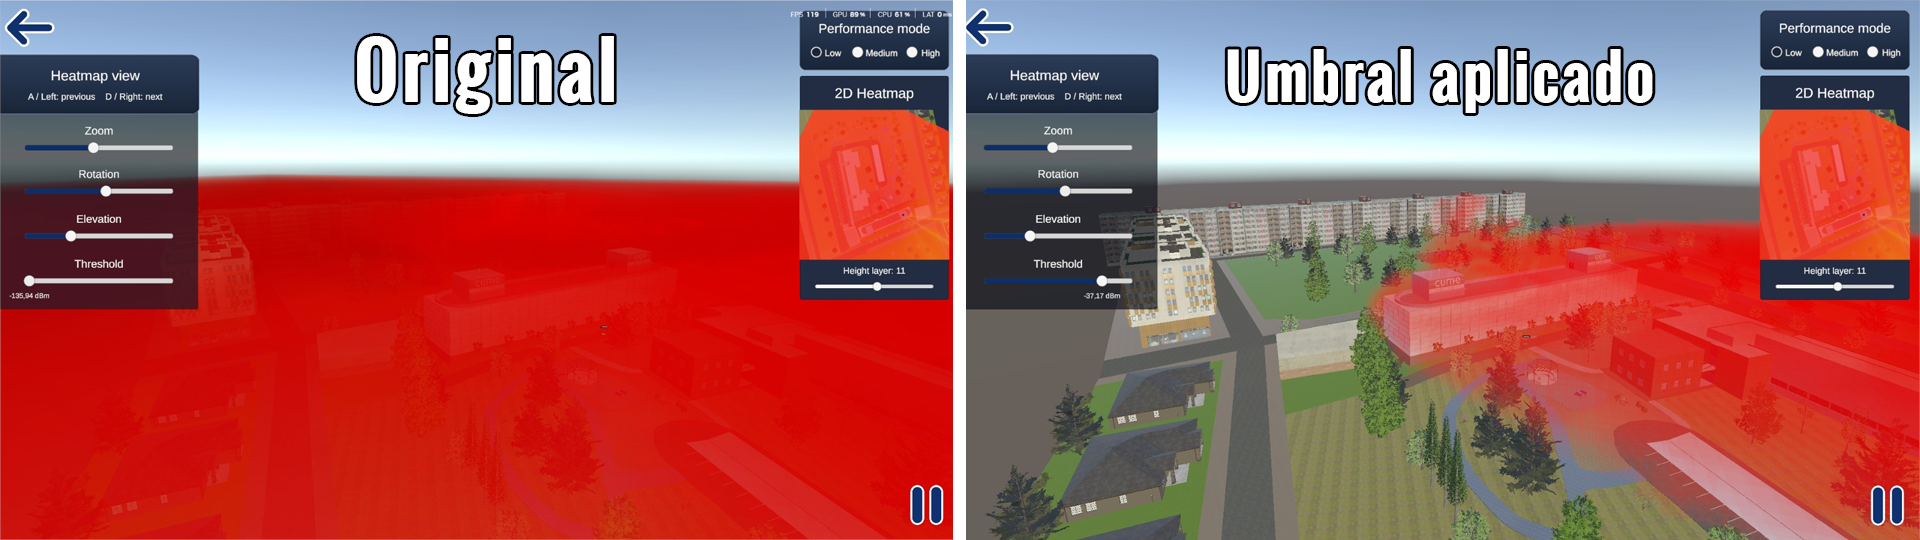
\includegraphics[width=1\textwidth, keepaspectratio]{imagenes/mapas de calor/umbral.png}
    \caption{Mapa de calor 3D con umbral de visualización aplicado}
    \label{fig:heatmap_umbral}
\end{figure}

Además del mapa 3D, se implementa una versión 2D por capas. Esta vista utiliza los mismos datos de la rejilla, pero muestra únicamente los vóxeles pertenecientes a una altura concreta. El usuario puede seleccionar la capa mediante un slider, y la textura del mapa se actualiza para mostrar la distribución de potencia recibida a esa altura.

Para generar el mapa 2D, se crea una textura sobre la que se pintan los vóxeles de la capa seleccionada. Cada vóxel se proyecta sobre el plano del mapa y se colorea según su potencia recibida normalizada. Como la rejilla puede estar rotada respecto al escenario, se calculan las esquinas del vóxel en el plano 2D y se rellena el área de píxeles correspondiente. 

Para evitar huecos visuales debidos al redondeo, se utiliza redondeo hacia abajo en los valores mínimos y redondeo hacia arriba en los valores máximos del área ocupada. Esta solución evita que queden espacios vacíos entre vóxeles debido al redondeo, aunque puede producir dientes de sierra en el minimapa 2D cuando el tamaño de vóxel utilizado es grande.

La vista 2D se genera a partir de una cámara ortográfica situada sobre el campus, que muestra una vista cenital del escenario. Para definir qué zona del escenario debe aparecer en esta imagen se utilizan dos puntos de referencia colocados en la escena, que marcan los límites del mapa. A partir de esos mismos límites, las posiciones de los vóxeles en coordenadas del mundo se convierten a coordenadas de píxel, permitiendo dibujar el mapa de calor exactamente sobre la zona correspondiente de la imagen cenital. De esta forma, el usuario puede relacionar la distribución de potencia recibida con los edificios, caminos y zonas del entorno. En la Figura \ref{fig:heatmap_2d_capas} se muestra un ejemplo del mapa de calor 2D por capas.

\begin{figure}[H]
    \centering
    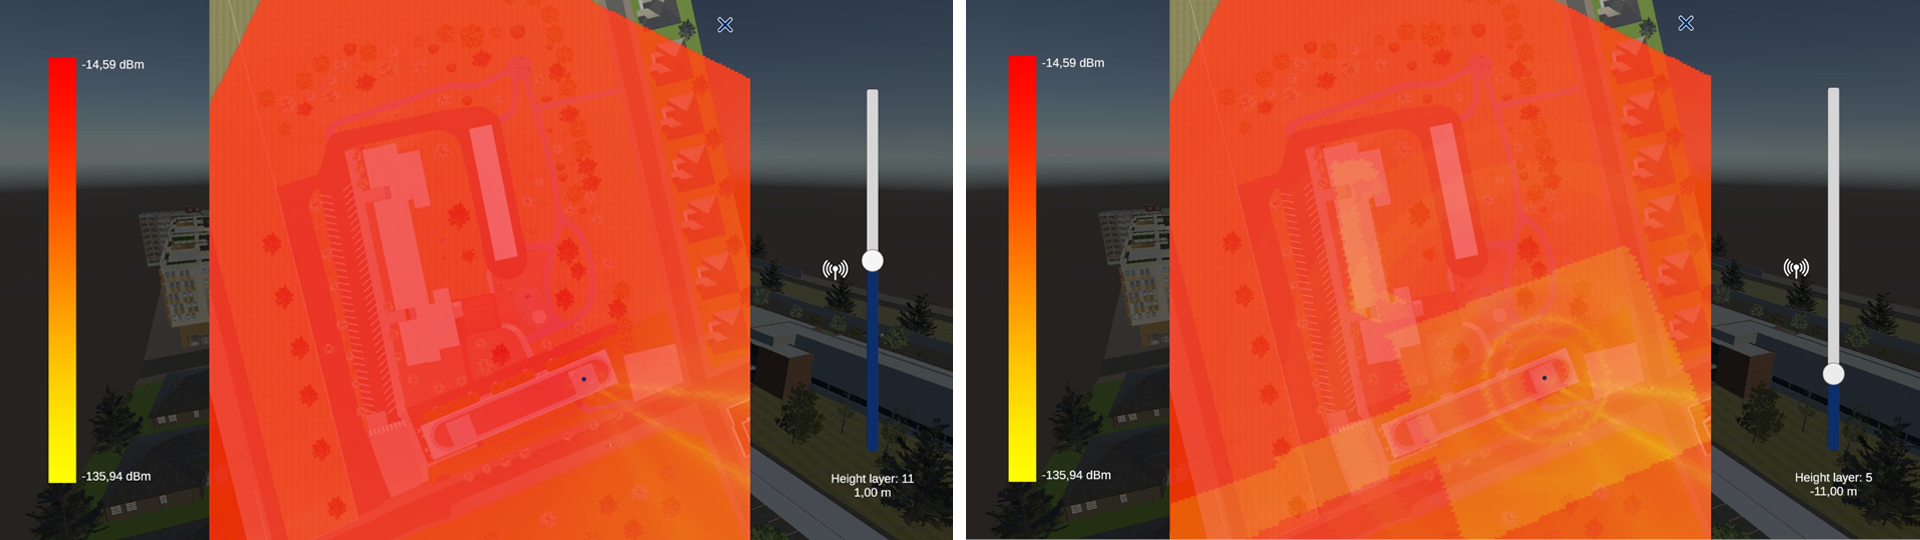
\includegraphics[width=1\textwidth, keepaspectratio]{imagenes/mapas de calor/mapa de calor 2d varias alturas.png}
    \caption{Mapa de calor 2D por capas}
    \label{fig:heatmap_2d_capas}
\end{figure}


\section{Receptores móviles, rutas y métricas}

Los receptores se desplazan por el escenario siguiendo rutas definidas previamente mediante puntos colocados en Unity. Cada ruta representa un tipo de recorrido diferente dentro del campus. De esta forma, la simulación no solo calcula la cobertura en puntos fijos, sino que también permite estudiar cómo varía la señal durante un recorrido.

En este trabajo se utilizan tres receptores móviles: un vehículo que recorre el campus, un vehículo con un recorrido lineal hacia la antena y un peatón. Al disponer de varios recorridos distintos, se pueden observar diferentes situaciones dentro del mismo escenario. El vehículo del campus representa un desplazamiento completo por todo el campus, el vehículo lineal permite analizar la evolución de la señal de forma lineal, y el peatón representa un caso de movimiento de un dispositivo 5G dentro del propio campus.

Cada receptor tiene asociada una ruta y una velocidad de movimiento en m/s. Durante la simulación, el receptor avanza de un punto de la ruta al siguiente. Al llegar a un punto, continúa hacia el siguiente hasta completar el recorrido. En el caso del vehículo del campus y el peatón, ambos realizan su ruta en bucle de forma ilimitada. No obstante, el vehículo lineal se detiene al llegar al final y se queda estacionado.

Los receptores también utilizan una ganancia de recepción configurable desde el menú inicial. Los vehículos emplean la ganancia definida para receptores vehiculares, mientras que el peatón utiliza la ganancia definida para receptores celulares. De esta forma, los valores pueden modificarse en función del caso que se quiera estudiar.

El movimiento de los receptores no comienza nada más cargar la escena. Antes de activarlos, el simulador espera a que se haya generado la rejilla de propagación y a que el servidor Python esté preparado para recibir peticiones. De esta forma, se evita que los receptores empiecen a recorrer la escena antes de que puedan calcular sus métricas.

Una vez que el sistema está preparado, se activa el movimiento de los receptores y comienza el registro de muestras. Durante el recorrido, Unity solicita periódicamente al servidor Python las métricas de cada receptor a partir de su posición actual. En la escena, esta actualización se realiza cada 0,05 segundos, por lo que se obtiene una secuencia de valores de potencia recibida, SNR, distancia al transmisor y pérdidas del enlace.

El registro de datos se detiene cuando el receptor completa su primer recorrido. Esto evita mezclar varias vueltas en una misma gráfica, ya que los datos serían equivalentes. Si la simulación se interrumpe antes de que un receptor termine su ruta, se exportan las muestras registradas hasta ese momento, evitando que se pierdan los datos obtenidos.

\section{Paneles de métricas y visualización de cobertura}

Los receptores móviles cuentan con paneles de métricas que muestran los valores calculados durante la simulación. Con cada nueva respuesta recibida desde Python se actualizan los valores mostrados en la interfaz, como la distancia al transmisor, la potencia recibida, la SNR, las pérdidas del enlace y el número de colisiones con edificios.

Junto con el panel de métricas, se implementa un visualizador de cobertura asociado a cada receptor móvil. Este visualizador muestra el estado de la cobertura a partir de la SNR obtenida en cada actualización. A primera vista, podría pensarse que el único umbral necesario es 0 dB, ya que la SNR representa la relación entre la potencia de señal y el ruido. En escala logarítmica, una SNR de 0 dB indica que la potencia de señal y la potencia de ruido son iguales, mientras que valores positivos indican que la señal está por encima del ruido.

Sin embargo, para representar la calidad de cobertura de forma más útil, no basta con distinguir únicamente entre valores positivos y negativos. Por este motivo, se buscó una referencia orientativa que permitiera separar distintos niveles de calidad de señal. La documentación de Cisco sobre resolución de problemas en interfaces celulares proporciona una tabla con rangos de calidad para RSSI, RSRP, RSRQ y SNR \cite{cisco_troubleshooting_cellular}. A partir de esa tabla se toman como referencia los límites de SNR de 20 dB, 13 dB y 0 dB.

Con estos umbrales se definen cuatro estados de cobertura: excelente para valores de SNR mayores o iguales que 20 dB, buena para valores entre 13 dB y 20 dB, aceptable para valores entre 0 dB y 13 dB, e insuficiente para valores menores que 0 dB. Estos límites no se interpretan como norma absoluta, sino que se utilizan como criterio visual para facilitar la interpretación de la cobertura durante la simulación.

El visualizador de cobertura está formado por un mensaje sobre el receptor y un indicador circular en el suelo. Cada vez que se reciben nuevas métricas, el sistema actualiza el texto y el color del indicador según el estado de cobertura calculado. De esta forma, el usuario puede identificar rápidamente la calidad del enlace sin depender únicamente del panel numérico.

\section{Generación automática de CSV y gráficas}

La generación de resultados se realiza durante la ejecución de la simulación. Cada receptor móvil tiene una lista con las muestras obtenidas durante su recorrido. De esta forma, los datos de los receptores no se mezclan entre sí y pueden exportarse de manera separada.

El registro de muestras comienza cuando la escena ya está preparada y los receptores empiezan a desplazarse. Cada vez que se reciben nuevas métricas desde el simulador Python, se guarda una muestra asociada al receptor correspondiente. 

Cuando un receptor completa su primer recorrido, se exportan las muestras almacenadas en un archivo CSV. Cada archivo contiene una cabecera con el nombre de las columnas y una fila por cada muestra registrada. Este archivo utiliza la coma como separador entre columnas y el punto como separador decimal. Además, los valores reales se guardan con tres decimales para facilitar su procesado posterior.

Una vez exportado el CSV de un receptor, se generan automáticamente las gráficas seleccionadas por el usuario en el menú de configuración. Para ello se utiliza el entorno Python integrado, que lee los datos exportados y crea las imágenes correspondientes en la misma carpeta de resultados.

Las gráficas generadas permiten analizar la potencia recibida y la SNR respecto a la distancia al transmisor, además de la evolución de la SNR respecto al tiempo. En esta última se añaden las líneas de los umbrales configurados y se calcula el porcentaje de tiempo en el que el receptor se mantiene por encima del límite de cobertura.

Además de exportar los resultados cuando un receptor completa su recorrido, la aplicación también tiene en cuenta el caso en el que la simulación se interrumpa antes de terminar. Si el usuario vuelve al menú o cierra la aplicación, se exportan igualmente las muestras disponibles hasta ese momento, evitando que se pierdan los datos ya registrados.

\section{Optimización y modos de rendimiento}

Durante el desarrollo del simulador, se añaden varias medidas para adaptar la aplicación a equipos con distintas capacidades. La escena principal está formada por un modelo tridimensional del campus, mapas de calor, receptores móviles, paneles de interfaz y comunicación periódica con el servidor Python, por lo que el rendimiento puede variar bastante según el ordenador utilizado.

Además de las optimizaciones de la representación del mapa de calor explicadas anteriormente, se añadieron modos de rendimiento configurables desde la interfaz. Estos modos permiten activar o desactivar elementos secundarios del escenario. En el modo de bajo rendimiento, se muestra el escenario completo. En el modo intermedio se oculta la vegetación, y en el modo de mayor rendimiento se ocultan la vegetación, el parque y los edificios de fondo.

Estos elementos mejoran el aspecto visual de la escena, pero no intervienen en los cálculos de propagación. Por este motivo, pueden desactivarse sin modificar los resultados de la simulación. De esta forma, el usuario puede reducir la carga gráfica cuando el dispositivo no sea capaz de ejecutar la escena con fluidez.

Otra medida aplicada es la limitación de los fotogramas por segundo (FPS). Sin esta limitación, la aplicación intenta generar el mayor número de FPS posible, aumentando innecesariamente el uso de CPU y GPU. Para evitarlo, se establece un límite en función de la frecuencia de refresco del monitor, pero sin superar los 120 FPS.

Con esta solución, en un monitor de 60 Hz, la aplicación se limita a 60 FPS, mientras que en monitores de mayor frecuencia se permite una tasa superior, hasta un máximo de 120 FPS. Esto evita fijar la aplicación a 60 FPS, lo que podría desaprovechar la fluidez de los monitores actuales, pero también impide que la simulación consuma recursos excesivos intentando alcanzar tasas de fotogramas demasiado altas.

\chapter{Pruebas y resultados}
\label{chap:pruebas_y_resultados}

En este capítulo se presentan las pruebas realizadas para comprobar el funcionamiento del simulador y analizar los resultados obtenidos en distintos casos de estudio.


\section{Escenario de pruebas}

Las pruebas se realizan sobre el escenario tridimensional del Centro Universitario de Mérida descrito en capítulos anteriores. La antena transmisora se mantiene en la parte superior del edificio administrativo, siguiendo la ubicación real tomada como referencia.

La configuración mostrada en la Tabla \ref{tab:parametros} se utiliza como caso base para el resto de pruebas. A partir de ella, se modifican algunos parámetros concretos, como el método de reconstrucción del patrón de radiación, el valor de k en el método de Vasiliadis y la potencia de transmisión.

\begin{table}[H]
    \centering
    \begin{tabularx}{\textwidth}{@{}llX@{}}
        \toprule
        \textbf{Parámetro} & \textbf{Valor}\\
        \midrule
        \texttt{Método de reconstrucción} & Vasiliadis, k = 2 \\
        \texttt{Potencia del transmisor} & 30 dBm \\
        \texttt{Frecuencia} & 1,785 GHz \\
        \texttt{Ancho de banda} & 10 MHz \\
        \texttt{Modelo de pérdidas} & FSPL \\
        \texttt{Shadowing} & Desactivado \\
        \texttt{Tamaño de la rejilla} & 300 x 40 x 400 m \\
        \texttt{Tamaño del vóxel} & 2 m \\
        \texttt{Ganancia receptores vehiculares} & 3 dBi \\
        \texttt{Ganancia receptor celular} & 0 dBi \\
        \bottomrule
    \end{tabularx}
    \caption{Parámetros de prueba}
    \label{tab:parametros}
\end{table}

La antena utilizada en el simulador es el modelo HWXX-6516DS1-VTM de Andrew. Según su ficha técnica, la antena trabaja en varias bandas dentro del rango de 1710 a 2690 MHz y admite una potencia máxima de 350 W por puerto~\cite{andrew_hwxx_datasheet}. Esta potencia máxima equivale aproximadamente a:

\[
P_{\mathrm{tx}}(\mathrm{dBm}) = 10 \log_{10}(350000) \approx 55,44\ \mathrm{dBm}
\]

En las pruebas no se utiliza la potencia máxima admitida por la antena, ya que este valor representa el límite físico que puede soportar el puerto de entrada y no una potencia habitual. En su lugar, se utiliza una potencia de transmisión de 30 dBm, equivalente a 1 W, como caso base para el escenario del campus. Este valor es inferior al límite indicado para una estación base de rango medio en ETSI TS 138 104, donde se define para las estaciones de rango medio una potencia menor o igual a 38 dBm \cite{etsi138104}. Además, al estar muy por debajo de los 350 W por puerto indicados en la ficha técnica, el valor seleccionado queda dentro del margen soportado por la antena.

La frecuencia seleccionada es 1,785 GHz. En la página del fabricante se encuentran disponibles distintos ficheros CSV con patrones de radiación medidos para varias frecuencias de operación de la antena \cite{andrew_hwxx_product}. En el simulador se utiliza el fichero correspondiente a 1,785 GHz. De esta forma, la frecuencia utilizada en los cálculos coincide con la frecuencia del patrón de radiación reconstruido.

El ancho de banda para todos los receptores es de 10 MHz. Este valor aparece tanto en las configuraciones de canal de 5G NR en FR1 \cite{etsi138104} como en comunicaciones vehiculares V2X \cite{etsi302663}. Como ambos casos pueden utilizar este ancho de banda, se ha utilizado el mismo valor para los receptores celulares y vehiculares, evitando diferentes anchos de banda en cada tipo de receptor.

Como modelo de pérdidas se utiliza FSPL. Se ha elegido este modelo como base para hacer todas las pruebas porque representa la propagación en espacio libre y permite comprobar los resultados de forma sencilla mediante fórmulas teóricas.

El \textit{shadowing} se desactiva en la configuración para garantizar que las simulaciones sean reproducibles. Al eliminar la componente aleatoria, dos ejecuciones con los mismos parámetros producen los mismos resultados, lo que facilita la validación del simulador y la comparación entre configuraciones.

La rejilla de simulación tiene un tamaño de $300 \times 40 \times 400$ m. Estas dimensiones son las mínimas para cubrir el campus al completo y poder analizar el mapa de calor en todo el escenario. Debido al gran tamaño de la rejilla, se utiliza un tamaño de vóxel de 2 m, ya que en caso de ser más pequeño el número de muestras sería excesivo para un ordenador de uso personal. En las pruebas donde se comparan mapas de calor a la altura del suelo se aumenta el alto de la rejilla de 40 a 50 para tener un margen más amplio.

En los receptores vehiculares se emplea una ganancia de 3 dBi, tomando como referencia los supuestos de simulación utilizados en estudios V2X de 3GPP~\cite{tr36885}. Para el receptor celular se utiliza una ganancia de 0 dBi para modelarlo como un terminal de usuario genérico. Este valor se toma como referencia a partir de ETSI TR 136 942~\cite{etsi136942}.

A partir de este caso base, se analizan variaciones según el patrón de radiación y la potencia de transmisión, observando su impacto sobre la potencia recibida, la SNR y la cobertura obtenida en el campus.

\section{Validación del patrón de radiación reconstruido}

Antes de utilizar el patrón de radiación en los cálculos de propagación, se realiza una prueba para comprobar que la reconstrucción implementada en Unity se ha realizado correctamente.

Para realizar esta comprobación, se crearon bolas de \textit{debug} dentro del simulador. Estas bolas se sitúan en el centro de cada vóxel de la rejilla y se utilizan únicamente durante las pruebas internas de desarrollo, por lo que el usuario final desconocerá su existencia. Su objetivo es permitir la inspección de los valores calculados en puntos concretos del escenario y comprobar que la reconstrucción del patrón de radiación funciona correctamente.

En la Figura \ref{fig:bolas_debug} se muestra un ejemplo de estas bolas de \textit{debug} colocadas sobre la rejilla de simulación. Cada bola representa un punto de la rejilla que puede seleccionarse para consultar los valores calculados en esa posición.

\begin{figure}[H]
    \centering
    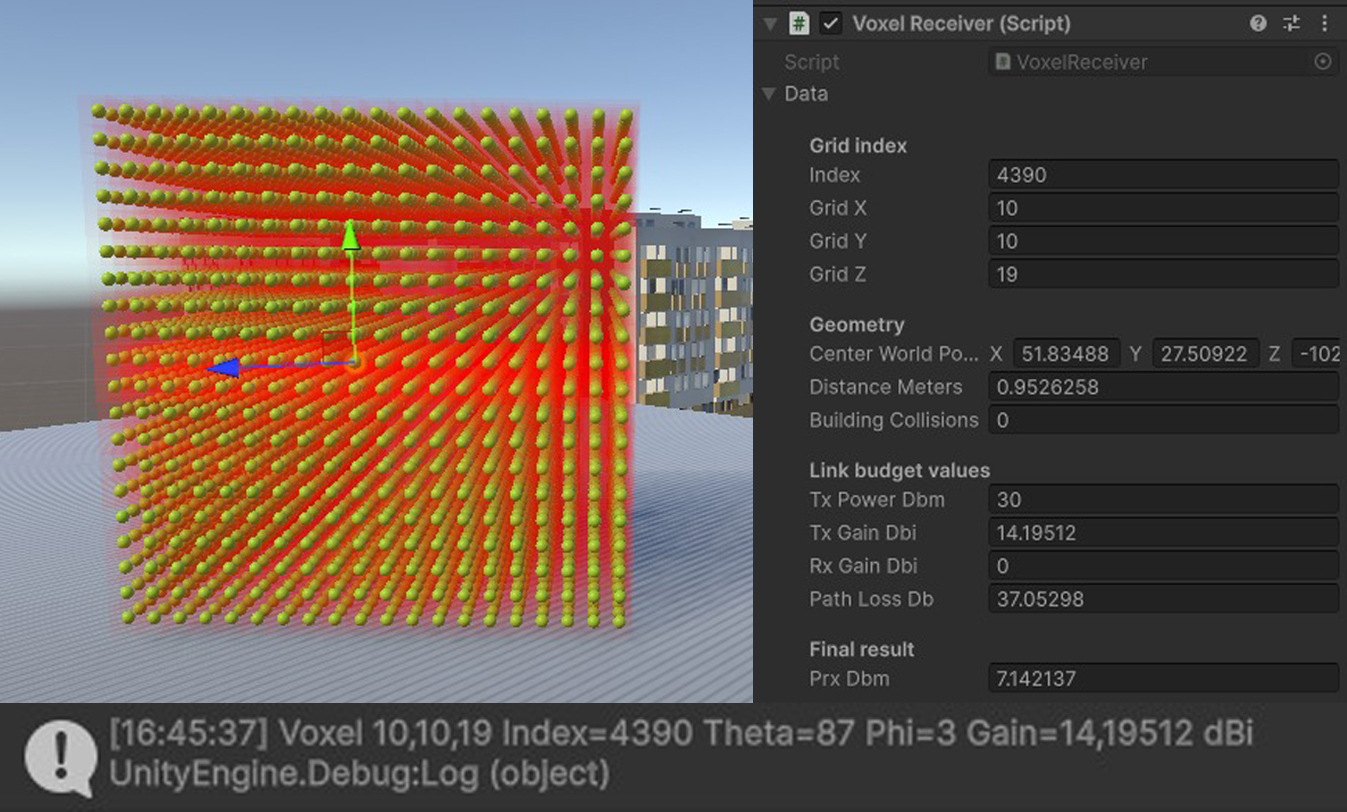
\includegraphics[width=0.85\textwidth, keepaspectratio]{imagenes/resultados/patron de radiacion/Bolas debug.jpg}
    \caption{Bolas de \textit{debug} utilizadas para inspeccionar valores de la rejilla}
    \label{fig:bolas_debug}
\end{figure}

Al hacer clic en una de estas bolas, el simulador muestra la información asociada a ese vóxel. Además, durante la generación de la rejilla, Unity muestra por consola un mensaje con el índice de cada bola y los ángulos theta y phi correspondientes a la dirección entre la antena y ese punto. Esta información permite realizar dos comprobaciones: por un lado, validar el cálculo de potencia recibida mediante el presupuesto de potencias y, por otro, comprobar que la ganancia del patrón de radiación se obtiene correctamente para esa dirección.

En primer lugar, se verifica el cálculo de potencia recibida en un punto concreto. Para ello, se utiliza la bola de \textit{debug} de la Figura \ref{fig:bolas_debug}, cuyo panel muestra una potencia recibida de $7,14$ dBm. Al tratarse de una prueba con el modelo FSPL y sin \textit{shadowing}, este valor puede comprobarse fácilmente mediante la expresión de pérdidas en el espacio libre \cite{itur_p341}:

\[
L_{\mathrm{FSPL}}(\mathrm{dB}) = 20 \log_{10}\left(\frac{4 \pi d f}{c}\right)
\]


donde $d$ es la distancia entre el transmisor y el receptor en metros, $f$ es la frecuencia en Hz y $c$ es la velocidad de la luz en m/s. A partir de esta pérdida, la potencia recibida se obtiene mediante el presupuesto de potencias:

\[
P_{\mathrm{rx}} = P_{\mathrm{tx}} + G_{\mathrm{tx}} + G_{\mathrm{rx}} - L_{\mathrm{FSPL}} - L_{\mathrm{edificios}}
\]

Para el punto seleccionado, el simulador muestra una distancia de $0,95$ m, una ganancia de transmisión de $14,20$ dBi, una ganancia de recepción de $0$ dBi y cero colisiones con edificios. Por tanto, las pérdidas adicionales por edificios son $0$ dB. Sustituyendo estos valores:

\[
L_{\mathrm{FSPL}} = 20 \log_{10}\left(\frac{4 \pi \cdot 0,95 \cdot 1,785 \cdot 10^9}{3 \cdot 10^8}\right) = 37,05\ \mathrm{dB}
\]

\[
P_{\mathrm{rx}} = 30 + 14,20 + 0 - 37,05 - 0 = 7,15\ \mathrm{dBm}
\]

Este valor coincide con el mostrado en la bola de \textit{debug}, donde se obtiene una potencia recibida de $7,14$ dBm. Esta comprobación permite verificar que el cálculo de pérdidas y el presupuesto de potencias se están aplicando correctamente.

Una vez comprobado el cálculo de potencia recibida, se validan las ganancias del patrón de radiación. Para ello, se utilizan los ángulos theta y phi asociados a cada bola de \textit{debug} y se comparan con una reconstrucción equivalente realizada en MATLAB mediante la función \texttt{patternFromSlices} \cite{mathworks_patternfromslices}. Así, para cada bola seleccionada, se compara la ganancia calculada por Unity con la ganancia obtenida en MATLAB para el mismo par de ángulos.

La comparación se realizó utilizando el método de Vasiliadis con dos valores distintos del parámetro $k$. Por un lado, se realizaron pruebas con $k = 1$ para observar el comportamiento de la reconstrucción con una ponderación más suave. Por otro lado, con $k = 2$, que es el valor utilizado como configuración base en el resto de pruebas del simulador.

En la Tabla \ref{tab:comprobacion_patron} se muestran los valores obtenidos para distintos pares de ángulos. Para cada dirección se incluye la ganancia calculada en MATLAB y los valores obtenidos en Unity con Vasiliadis para $k = 1$ y $k = 2$.

\begin{table}[H]
    \centering
    \begin{tabularx}{\textwidth}{@{}ccXXX@{}}
        \toprule
        \textbf{$\theta$} & \textbf{$\phi$} & \textbf{MATLAB (dBi)} & \textbf{Unity $k=1$ (dBi)} & \textbf{Unity $k=2$ (dBi)}\\
        \midrule
        90 & 25 & 14,25 & 14,25 & 14,25 \\
        90 & 68 & 6,80 & 6,80 & 6,80 \\
        90 & 180 & -18,82 & -18,82 & -18,82 \\
        135 & 0 & 3,71 & 3,70 & -3,71 \\
        87 & 3 & 14,20 & 14,34 & 14,20 \\ % 4390
        48 & 245 & -15,77 & -7,38 & -15,77 \\ % 7700
        93 & 165 & -19,89 & -19,88 & -19,89 \\ % 3612
        138 & 315 & 0,63 & -1,30 & 0,63 \\ % 704
        72 & 65 & -10,37 & -9,97 & -10,37 \\ % 5499
        168 & 198 & -28,03 & -14,97 & -28,03 \\ % 969
        \bottomrule
    \end{tabularx}
    \caption{Comparación de ganancias del patrón reconstruido}
    \label{tab:comprobacion_patron}
\end{table}

Los resultados muestran que los valores obtenidos en Unity con el método de Vasiliadis y $k = 2$ coinciden con los obtenidos en MATLAB para los ángulos analizados. Esto confirma que la implementación utilizada en el simulador reproduce correctamente la reconstrucción tomada como referencia. En cambio, al utilizar $k = 1$ se obtiene un rango de ganancias más reducido entre los valores máximos y mínimos, por lo que el patrón reconstruido presenta variaciones más leves. Por este motivo, se utiliza $k = 2$ como valor base en el resto de pruebas.

Además, los primeros ángulos de la tabla son direcciones pertenecientes a los cortes horizontal y vertical del fichero CSV original, por lo que no dependen de la reconstrucción. Estos casos sirven como comprobación de que la lectura del fichero de antena y la conversión de ángulos utilizada en Unity son correctas. Los valores obtenidos coinciden con los del CSV original, lo que confirma que el simulador funciona correctamente.

En la Figura \ref{fig:patron_matlab} se muestra visualmente la comparación entre el patrón reconstruido en Unity mediante el método de Vasiliadis con $k = 2$ y el patrón obtenido en MATLAB. En ambos casos se aprecia una forma muy similar del lóbulo principal y de las zonas de menor ganancia, lo que confirma que la reconstrucción no solo coincide en los puntos numéricos comprobados, sino también en la forma general del patrón tridimensional.

\begin{figure}[H]
    \centering
    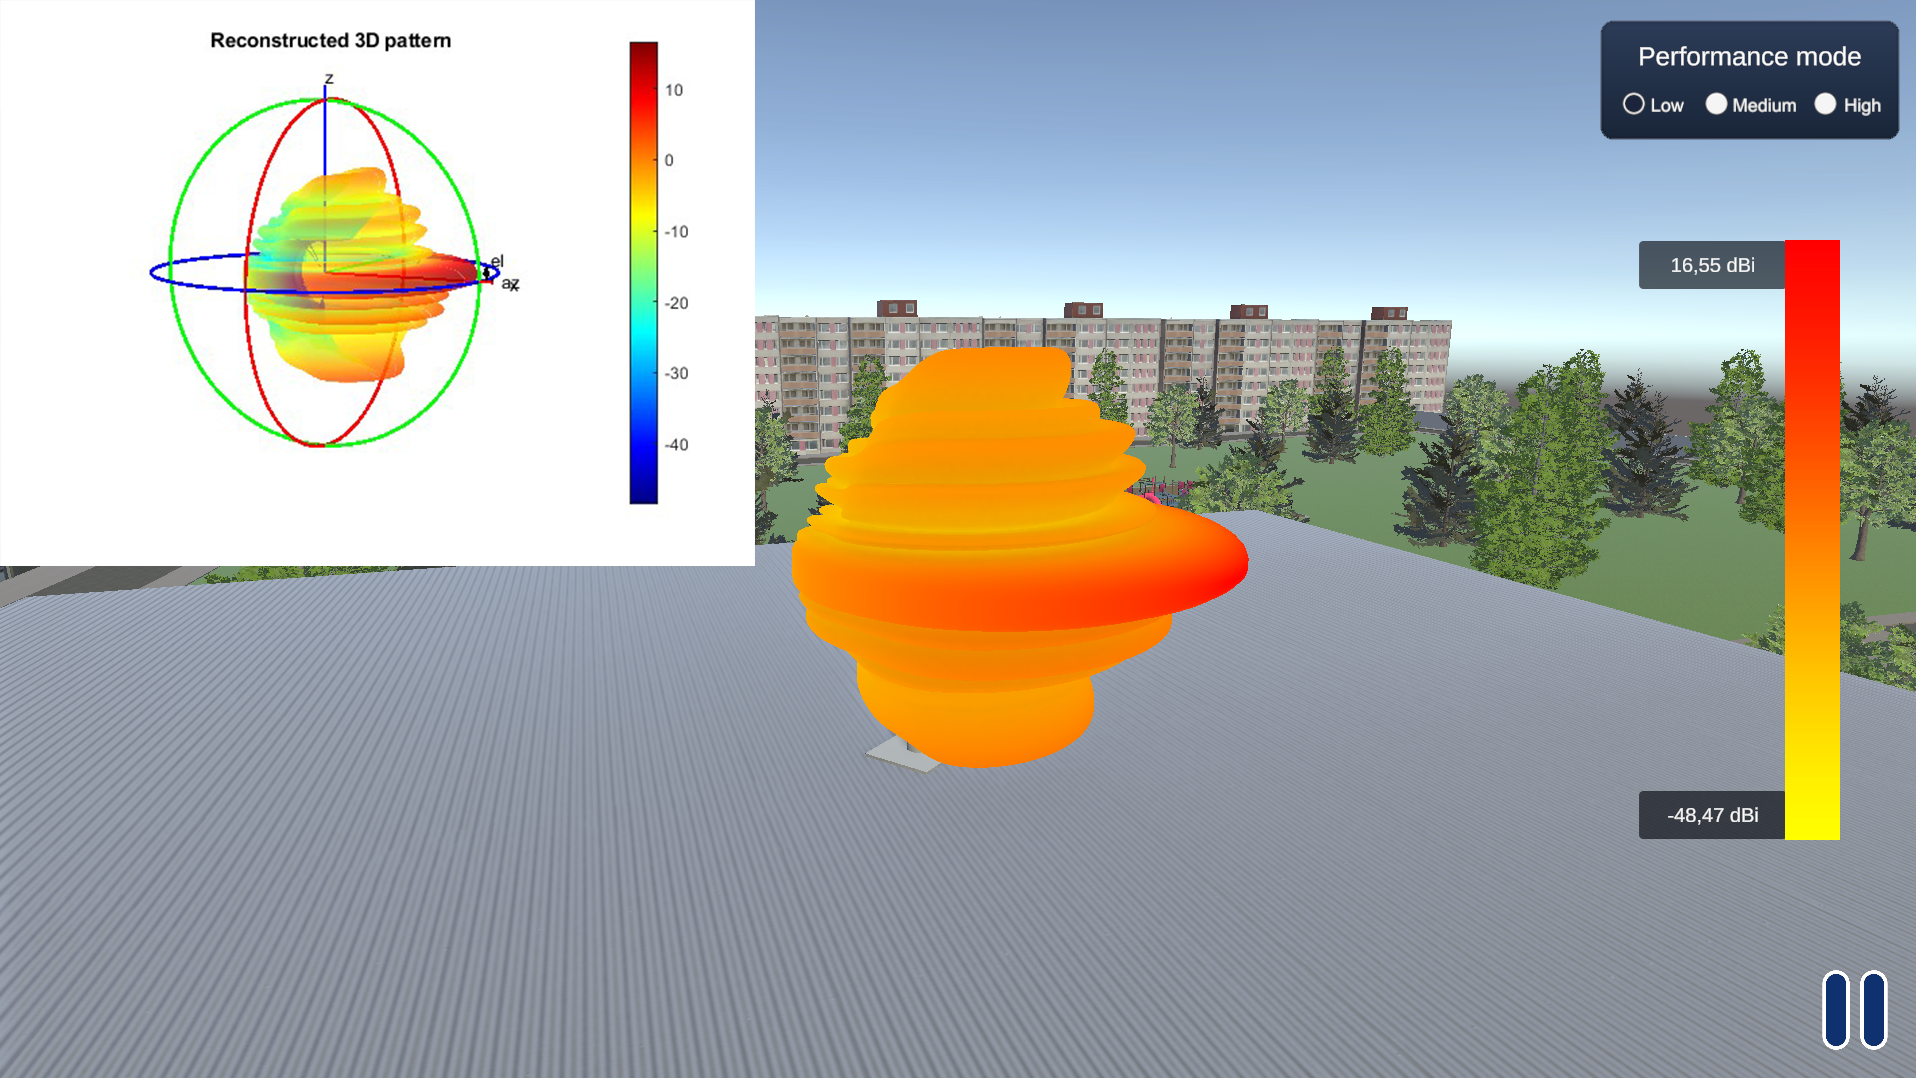
\includegraphics[width=1\textwidth, keepaspectratio]{imagenes/resultados/patron de radiacion/patron de radiacion.PNG}
    \caption{Comparación del patrón reconstruido con el de MATLAB}
    \label{fig:patron_matlab}
\end{figure}

Esta prueba también permite validar que la conversión entre posiciones del escenario y ángulos del patrón se realiza correctamente. Por tanto, el patrón reconstruido puede utilizarse posteriormente en los cálculos de propagación, ya que el simulador es capaz de obtener la ganancia de transmisión correspondiente a cada dirección del espacio.


\section{Resultados rejilla de propagación}

En esta sección se muestran los resultados obtenidos al calcular la rejilla tridimensional de vóxeles. En primer lugar, se representa una rejilla reducida de $50 \times 40 \times 50$ m, ya que este tamaño permite apreciar con claridad la distribución de la potencia recibida alrededor de la antena. Al ser el número total de vóxeles muy reducido, se puede apreciar fácilmente sin necesidad de utilizar el umbral o el mapa en dos dimensiones.

En la Figura \ref{fig:heatmap_3d_reducido} se puede ver cómo la potencia recibida no se distribuye de forma uniforme en todas las direcciones. Las zonas con mayor intensidad de rojo se corresponden con las zonas de mayor potencia recibida, mientras que las zonas más alejadas o en direcciones de bajas ganancias en el patrón de radiación tienen valores más oscuros y transparentes.

\begin{figure}[H]
    \centering
    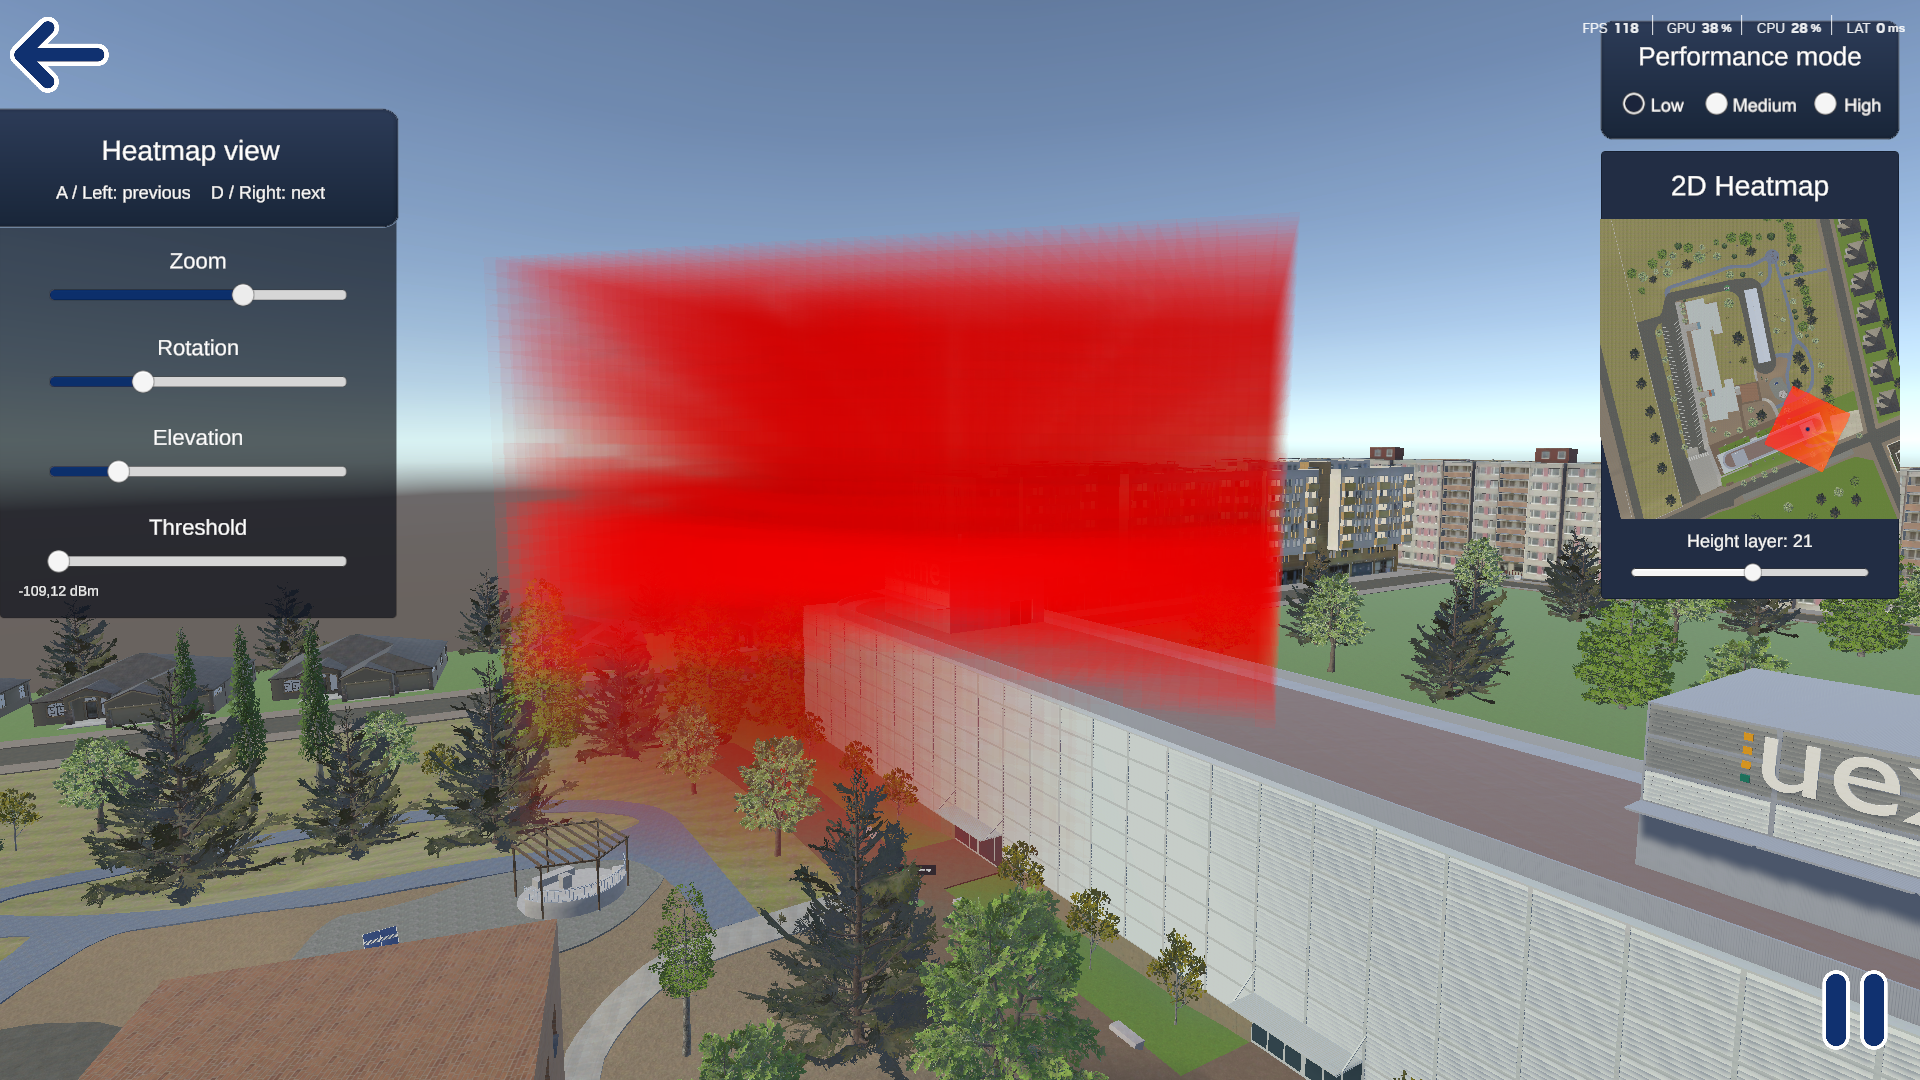
\includegraphics[width=1\textwidth, keepaspectratio]{imagenes/resultados/mapas de calor/Mapa de calor 50x40x50.PNG}
    \caption{Mapa de calor 3D para una rejilla reducida de $50 \times 40 \times 50$ m}
    \label{fig:heatmap_3d_reducido}
\end{figure}

Sin embargo, cuando se utiliza la rejilla del caso base para cubrir todo el campus, la visualización tridimensional contiene un número mucho mayor de vóxeles. En este caso, aunque el resultado sigue siendo útil para observar la cobertura general, la densidad de puntos dificulta la interpretación directa del mapa completo.

Como se observa en la Figura \ref{fig:heatmap_3d_campus}, al representar todo el campus, el número de vóxeles aumenta considerablemente y la visualización resulta imposible de analizar. Por este motivo, en la siguiente representación se hace uso del umbral de visualización, ocultando los vóxeles con menor potencia recibida y manteniendo visibles únicamente las zonas con valores más altos.

\begin{figure}[H]
    \centering
    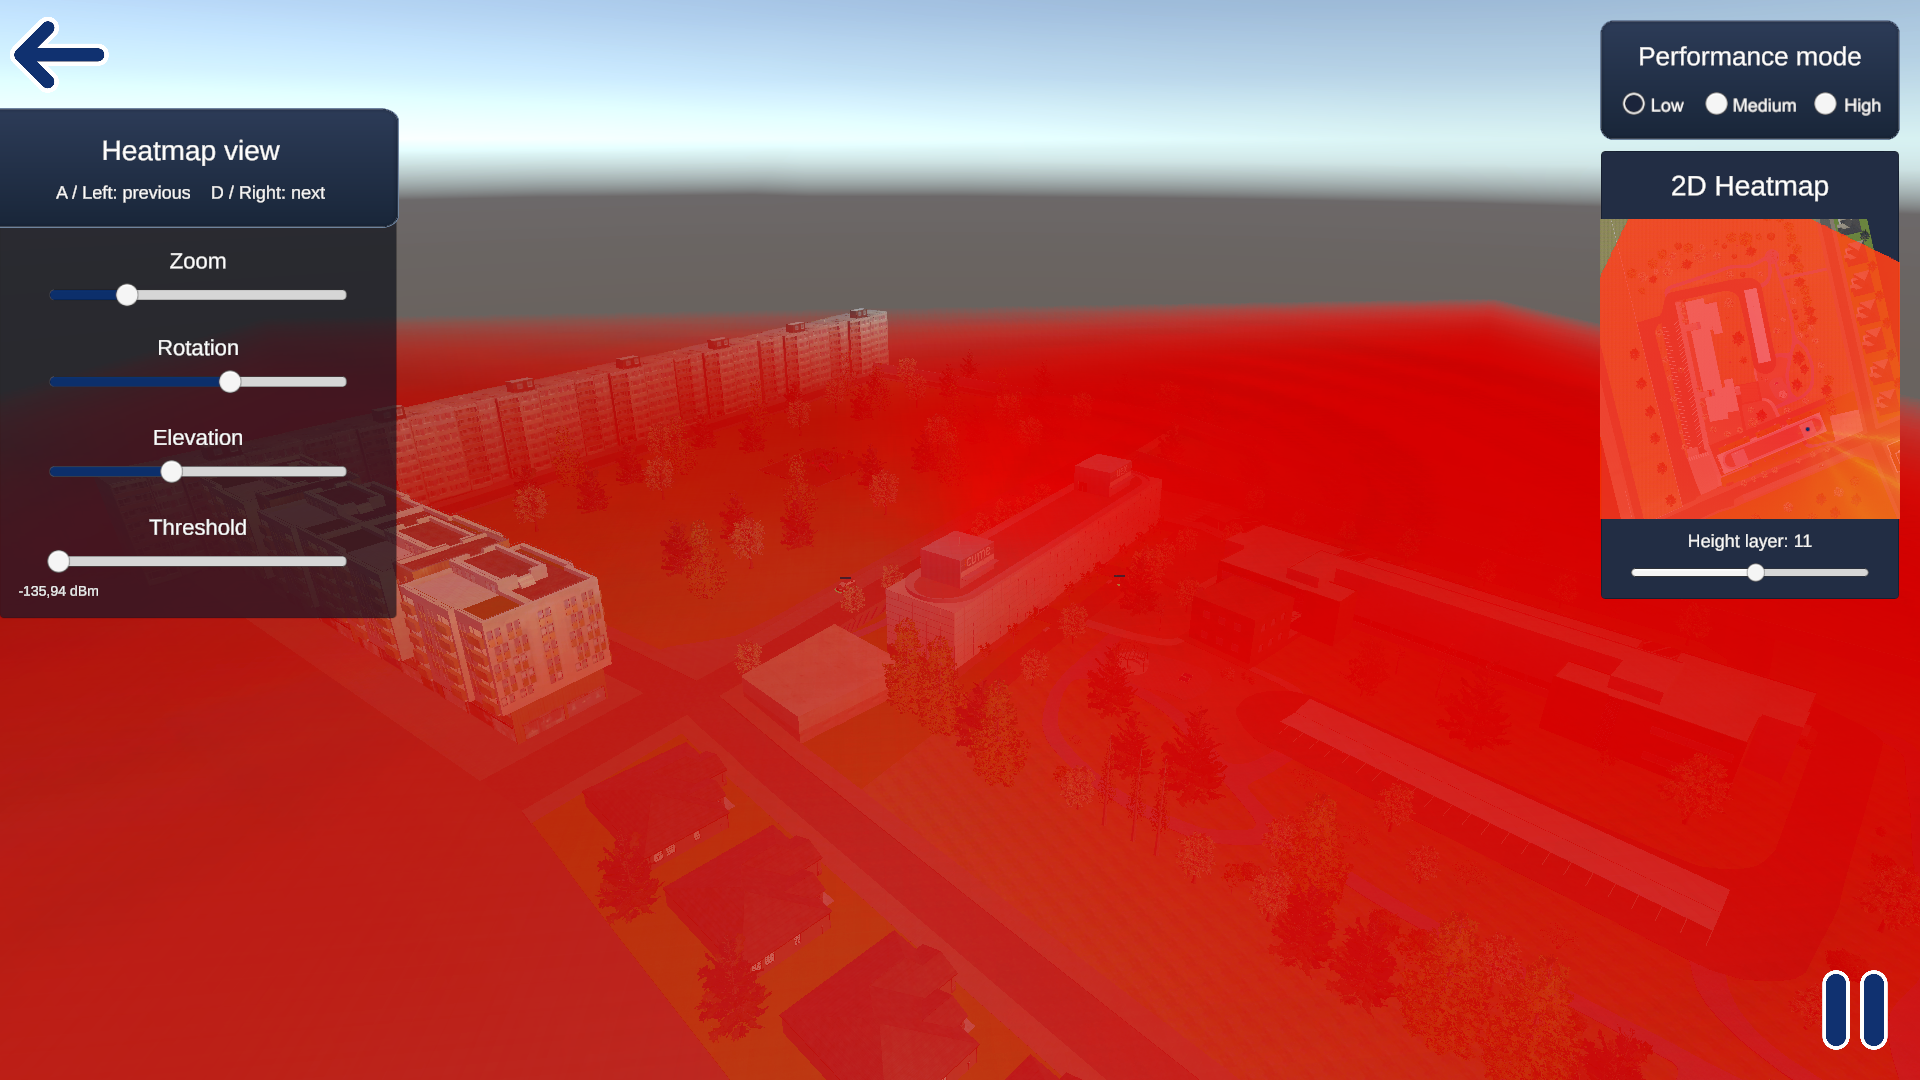
\includegraphics[width=1\textwidth, keepaspectratio]{imagenes/resultados/mapas de calor/Mapa de calor saturado.PNG}
    \caption{Mapa de calor 3D para la rejilla completa del campus}
    \label{fig:heatmap_3d_campus}
\end{figure}

En la Figura \ref{fig:heatmap_3d_umbral} se muestra cómo el uso del umbral facilita la visualización de las zonas con mayor potencia recibida. Esta representación permite distinguir con mayor claridad las regiones principales de cobertura, especialmente alrededor de la antena y en las direcciones donde el patrón de radiación presenta una mayor ganancia.

\begin{figure}[H]
    \centering
    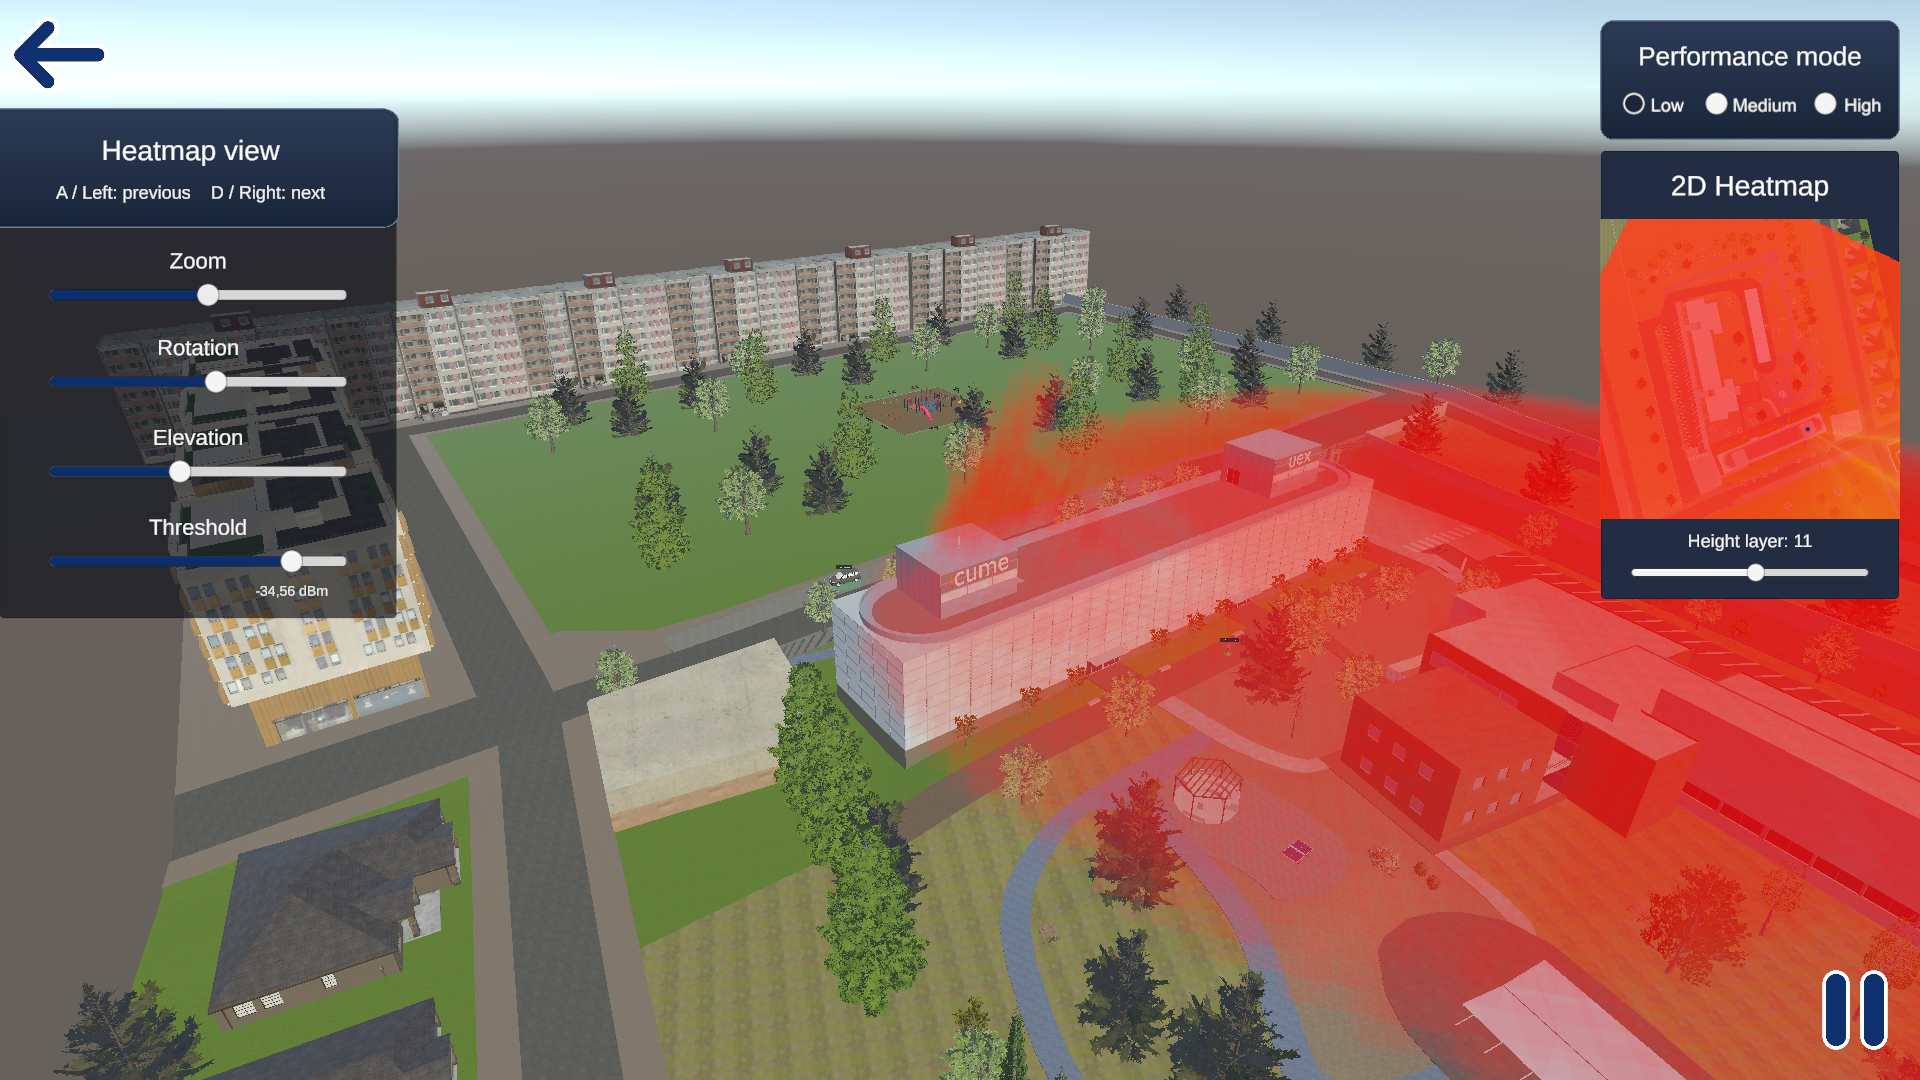
\includegraphics[width=1\textwidth, keepaspectratio]{imagenes/resultados/mapas de calor/Mapa de calor saturado con umbral.PNG}
    \caption{Mapa de calor 3D de la rejilla completa aplicando umbral de visualización}
    \label{fig:heatmap_3d_umbral}
\end{figure}

Además de la representación tridimensional, se utiliza el mapa de calor 2D por capas para estudiar la cobertura en planos horizontales concretos. Esta vista es muy práctica para analizar la rejilla completa, ya que permite estudiar el comportamiento de la señal a una altura determinada evitando el problema de la superposición de vóxeles.

En la Figura \ref{fig:heatmap_2d_campus} se aprecia con mayor detalle la distribución de potencia recibida sobre el campus. Las zonas próximas a la antena y con trayectorias más despejadas presentan valores más altos, mientras que alrededor de algunos edificios se observa una reducción notable de la potencia. Esta disminución se debe a las pérdidas adicionales introducidas cuando la trayectoria entre el transmisor y el punto receptor atraviesa los \textit{colliders} de los edificios.

\begin{figure}[H]
    \centering
    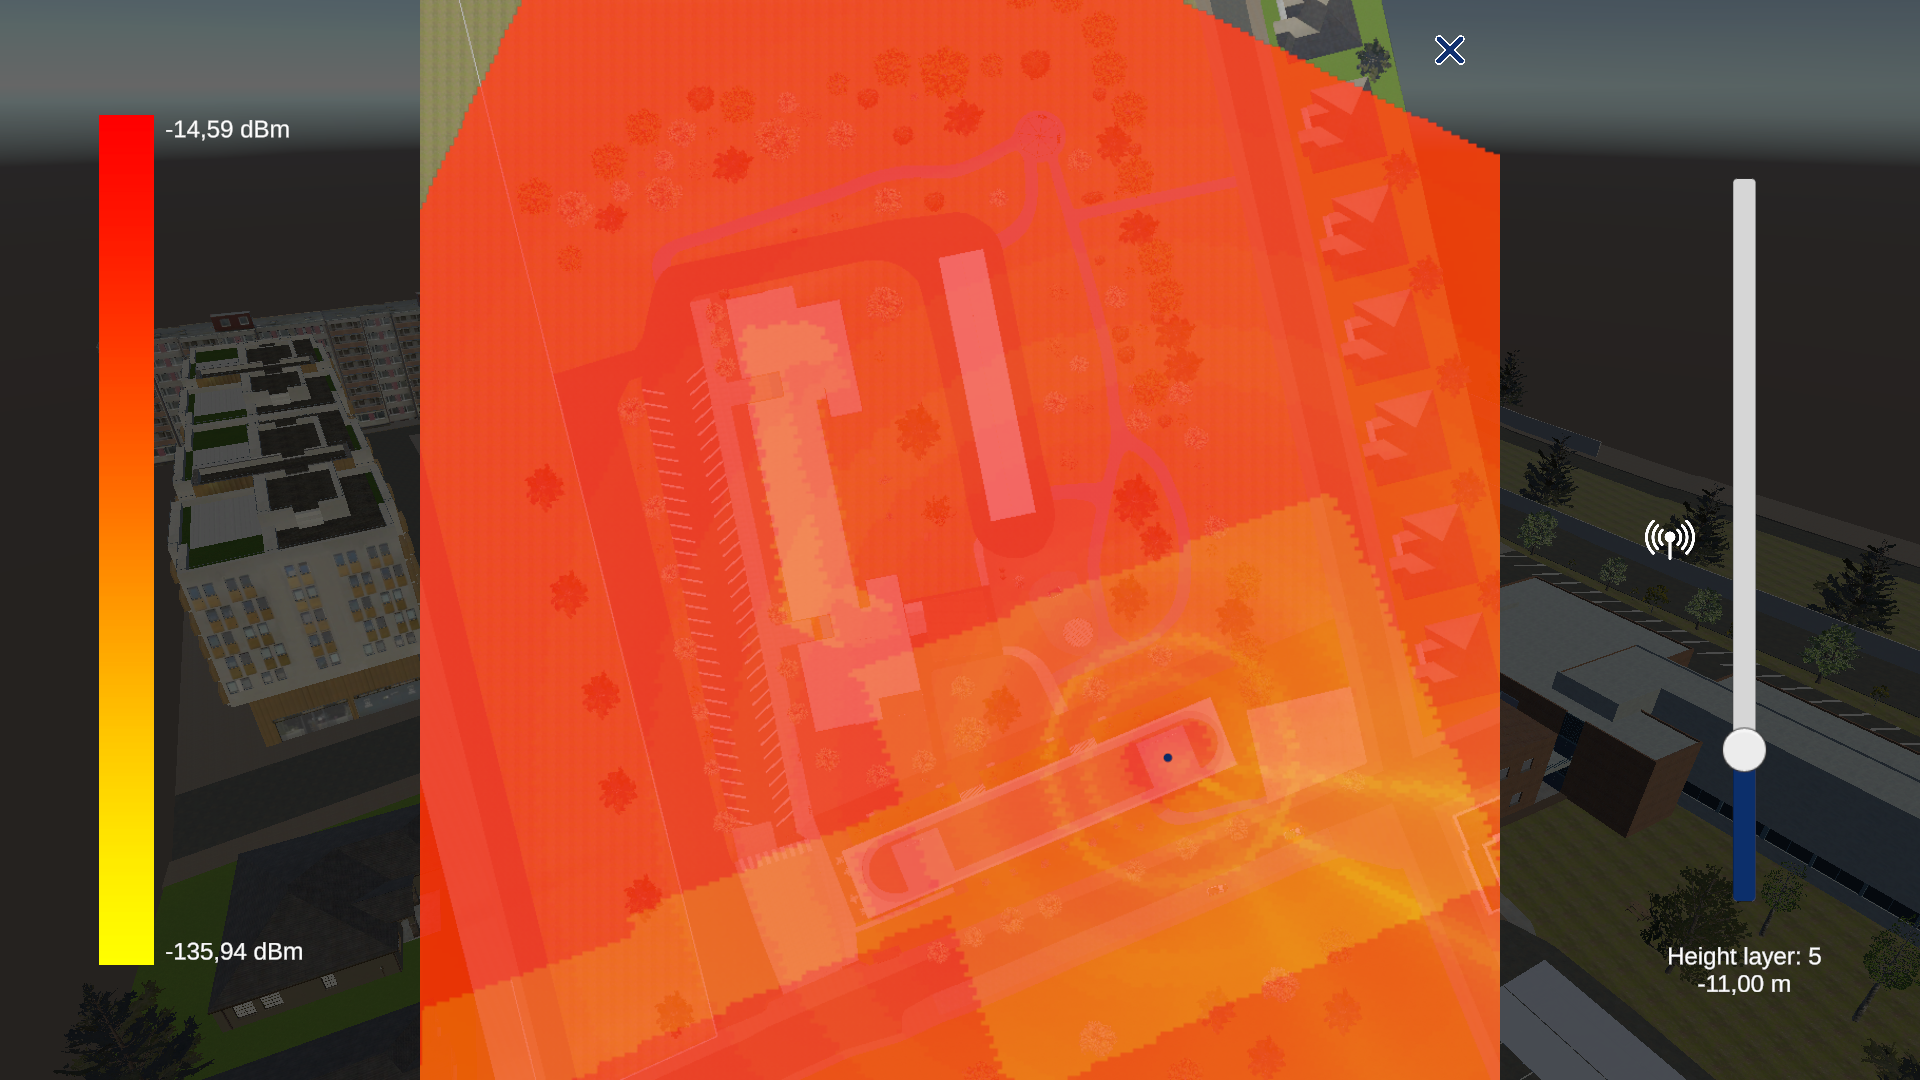
\includegraphics[width=1\textwidth, keepaspectratio]{imagenes/resultados/mapas de calor/Mapa de calor 2D bajo.PNG}
    \caption{Mapa de calor 2D por capas sobre el escenario del campus}
    \label{fig:heatmap_2d_campus}
\end{figure}

Este comportamiento confirma que el mapa de calor no depende únicamente de la distancia a la antena. También influyen la dirección respecto al patrón de radiación y la presencia de obstáculos en el escenario. Por esto, dos puntos situados a la misma distancia del transmisor pueden tener distinta potencia recibida si uno de ellos se encuentra en una zona más alineada con el lóbulo principal o si la señal atraviesa edificios antes de llegar.

En conjunto, estos resultados muestran que la rejilla tridimensional permite obtener una visión general de la cobertura en el campus, mientras que el mapa 2D por capas facilita el análisis detallado de zonas concretas. La combinación de ambas vistas permite interpretar mejor cómo se distribuye la potencia recibida en el escenario y cómo afectan tanto el patrón de radiación como los obstáculos presentes.


\section{Resultados de receptores móviles}

Una vez generada la rejilla de propagación, se activan los receptores móviles y comienzan a actualizarse sus métricas durante el recorrido. En este apartado se muestran los resultados obtenidos con la configuración base, centrándose en la visualización dentro del simulador y en la interpretación de las métricas mostradas en tiempo real.

En las Figuras \ref{fig:metricas_Vehiculo_campus}, \ref{fig:metricas_vehiculo_lineal} y \ref{fig:metricas_peaton} se muestran ejemplos de las vistas asociadas a los tres receptores móviles. Cada vista permite seguir al receptor seleccionado y consultar sus métricas principales, como la distancia al transmisor, la potencia recibida, la SNR, las pérdidas del enlace y el número de colisiones con edificios.

\begin{figure}[H]
    \centering
    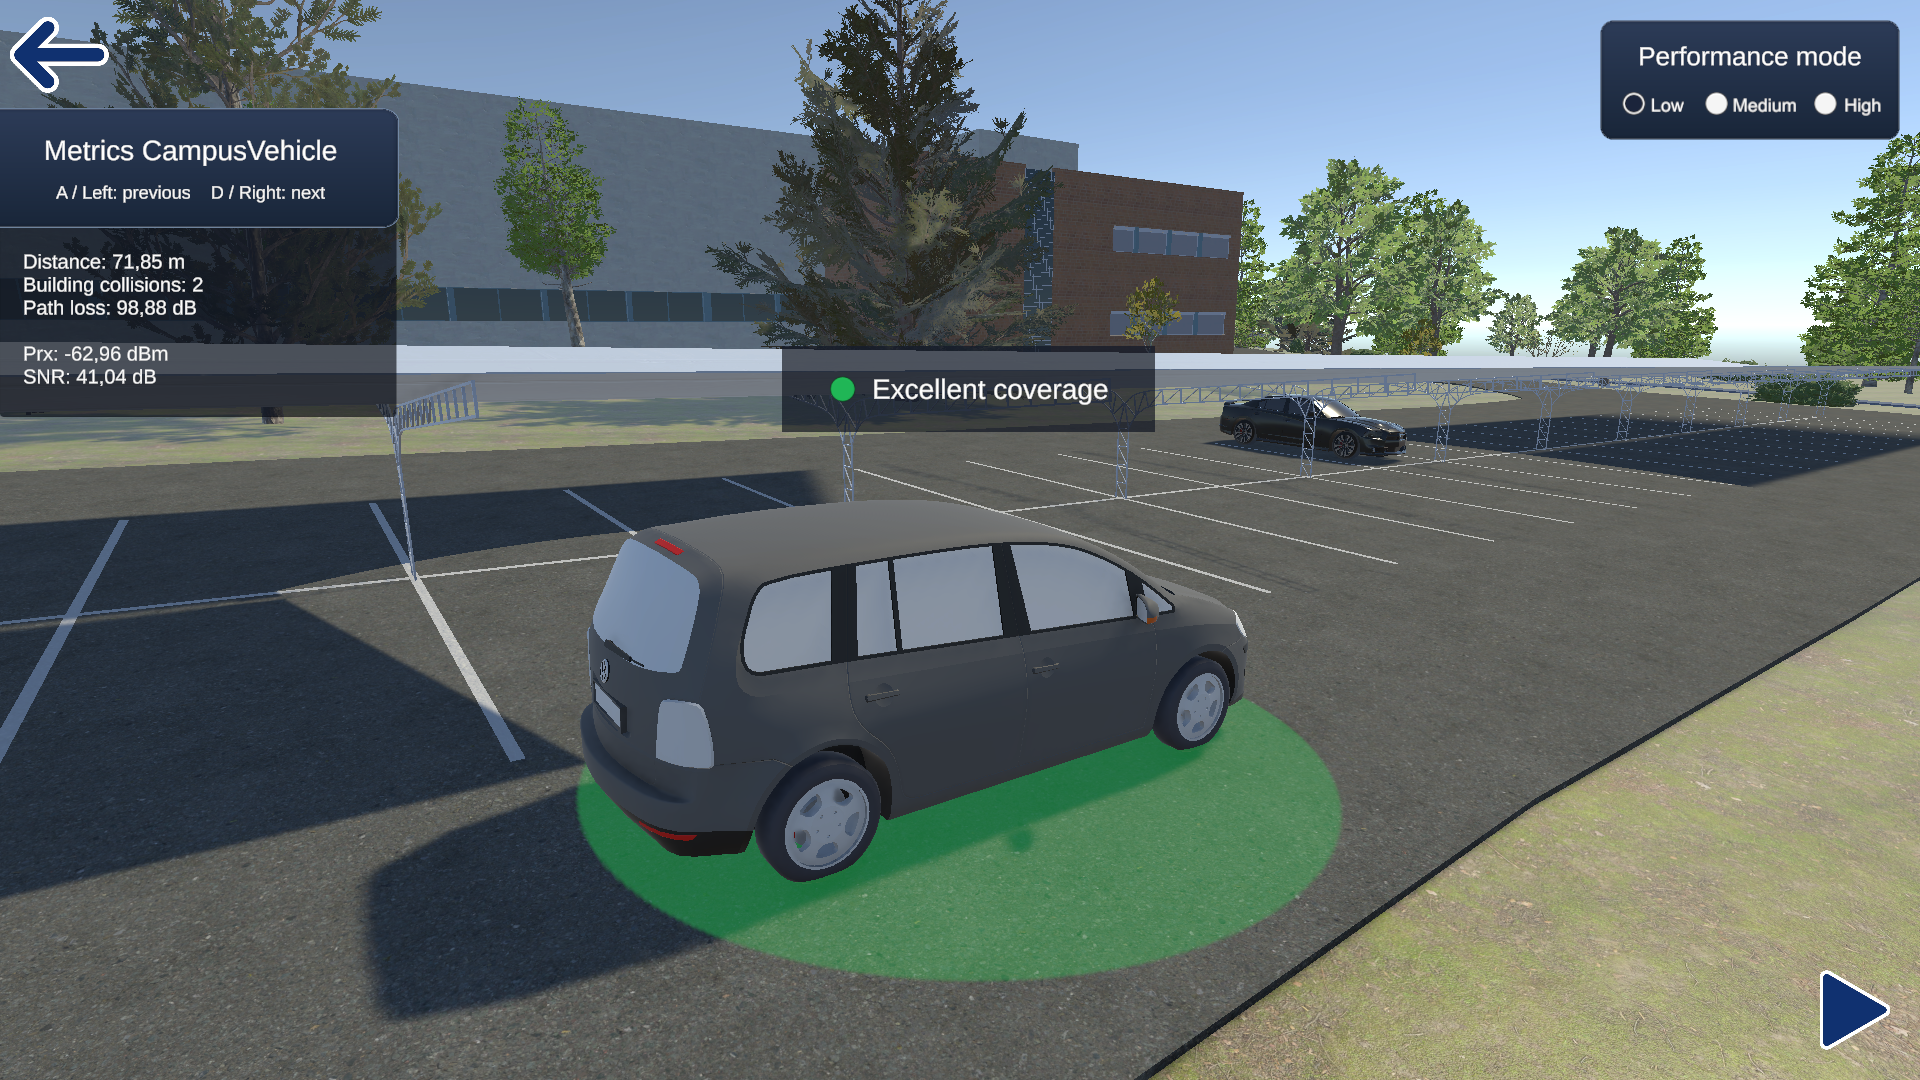
\includegraphics[width=1\textwidth, keepaspectratio]{imagenes/resultados/receptores moviles/vehiculo campus excelente.PNG}
    \caption{Vista del receptor CampusVehicle}
    \label{fig:metricas_Vehiculo_campus}
\end{figure}

\begin{figure}[H]
    \centering
    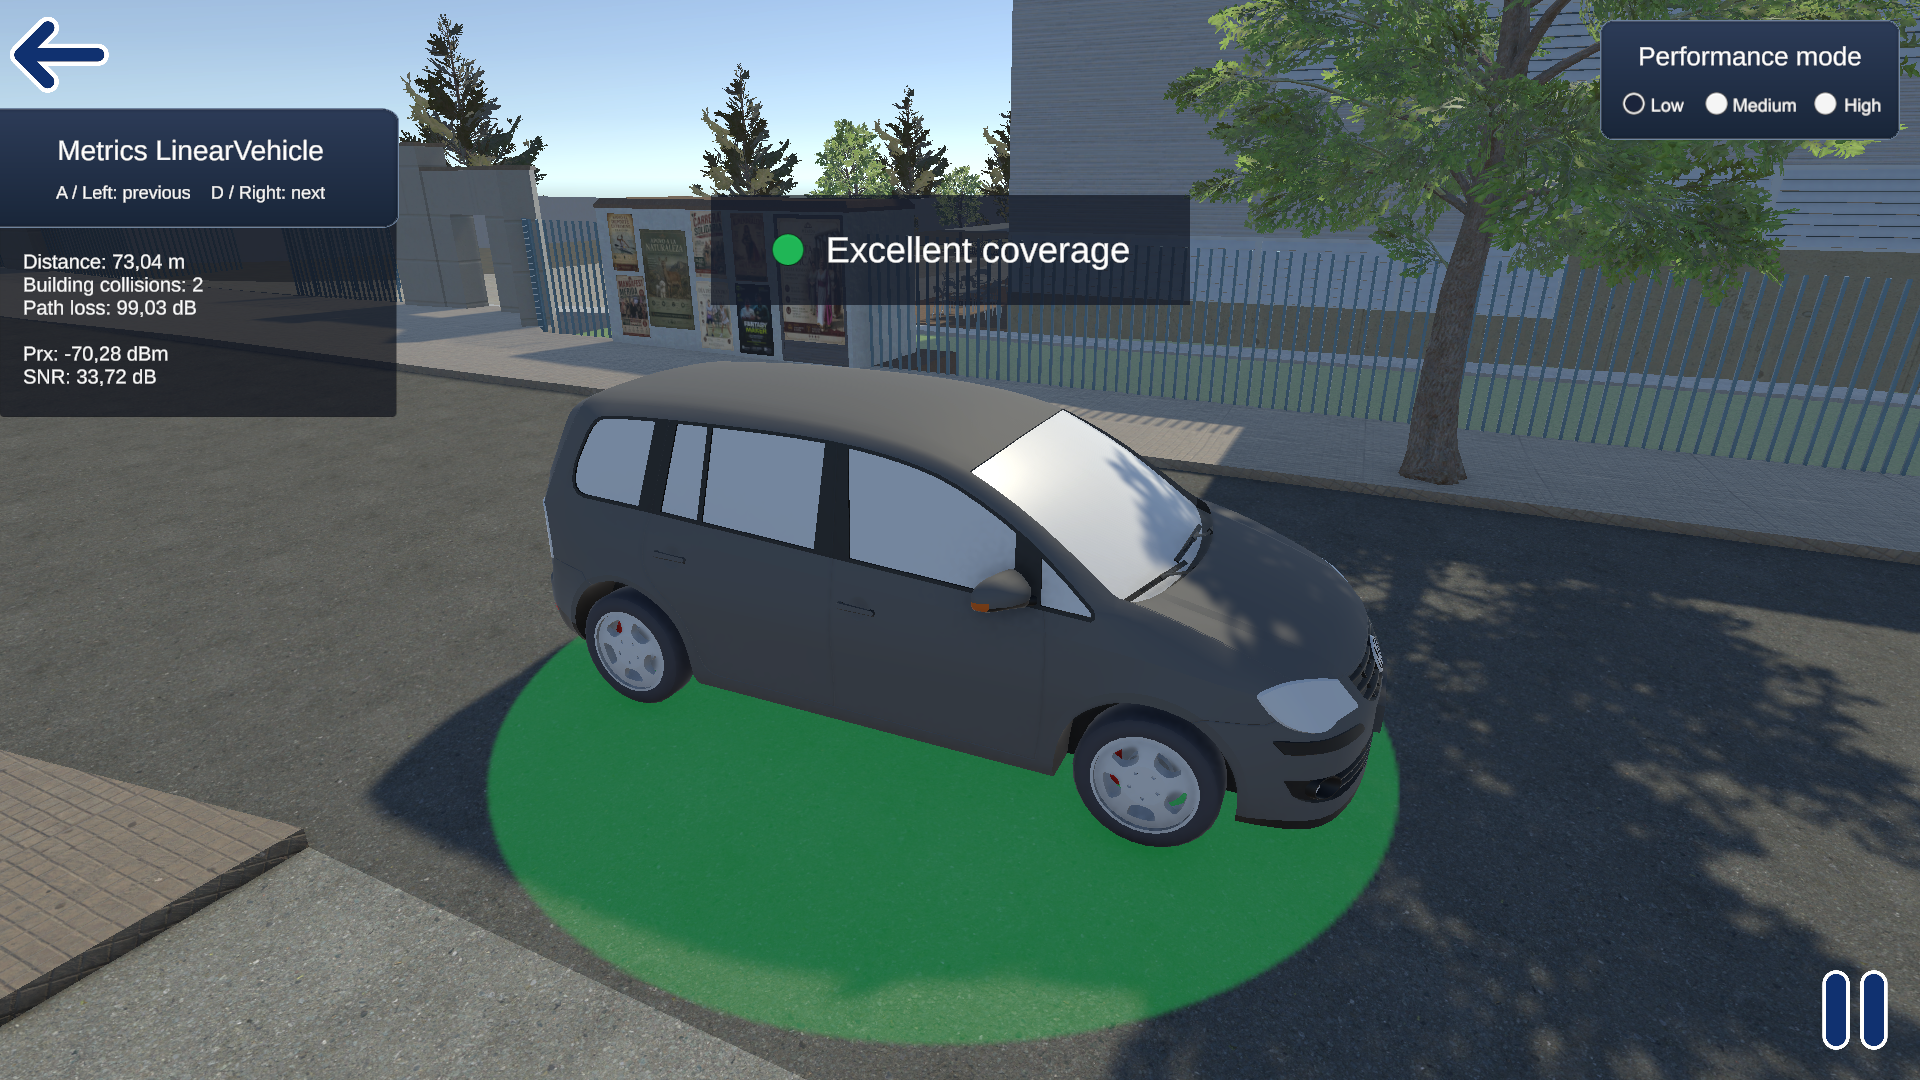
\includegraphics[width=1\textwidth, keepaspectratio]{imagenes/resultados/receptores moviles/vehiculo lineal excelente.PNG}
    \caption{Vista del receptor LinearVehicle}
    \label{fig:metricas_vehiculo_lineal}
\end{figure}

\begin{figure}[H]
    \centering
    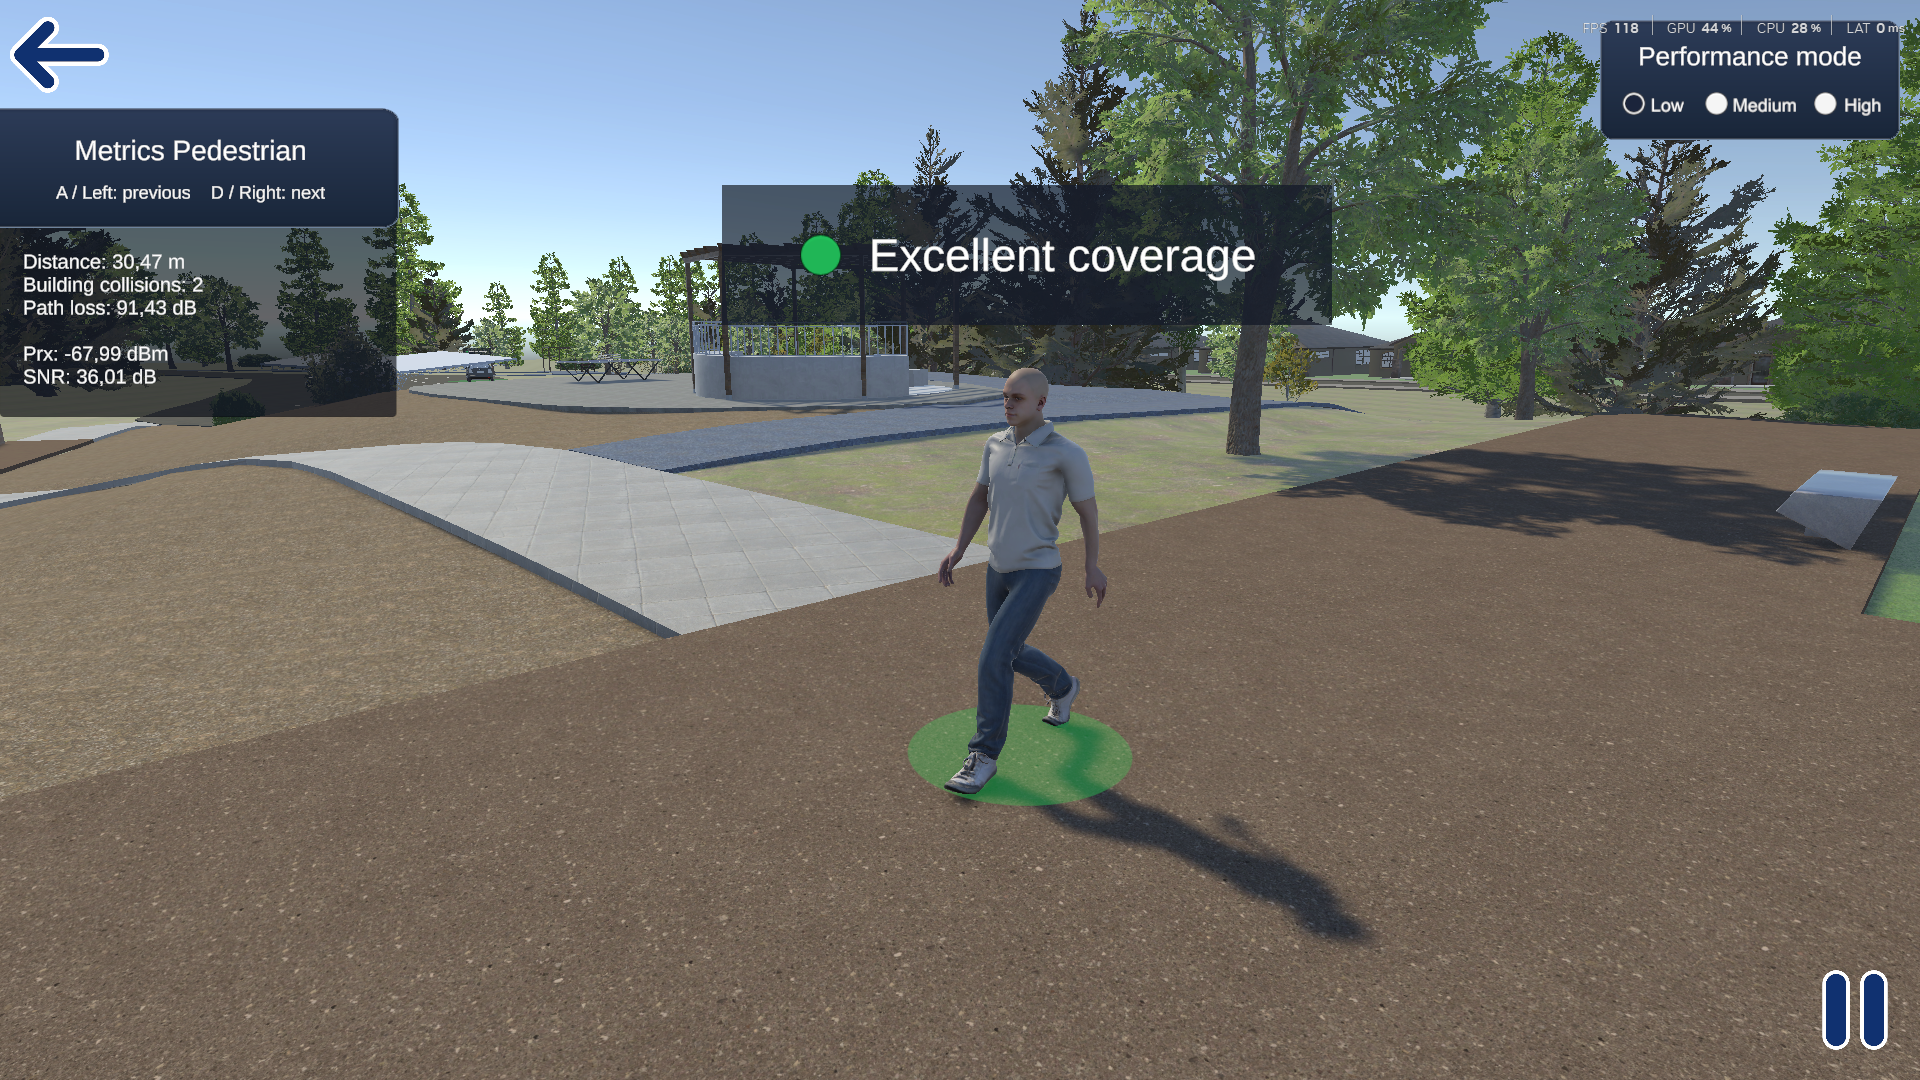
\includegraphics[width=1\textwidth, keepaspectratio]{imagenes/resultados/receptores moviles/peaton excelente.PNG}
    \caption{Vista del receptor Pedestrian}
    \label{fig:metricas_peaton}
\end{figure}

Aunque los tres receptores utilizan la misma configuración de propagación, los valores mostrados no evolucionan de la misma forma. Esto se debe a que cada receptor se desplaza por una zona distinta del escenario y, por tanto, cambia su distancia al transmisor, su orientación respecto al patrón de radiación y el número de obstáculos que la señal atraviesa. Además, los receptores vehiculares utilizan una ganancia de recepción mayor que la del receptor peatonal, lo que también influye en la potencia recibida.

Durante el recorrido, aparece un caso puntual en el que la cobertura cae de forma muy clara. En la Figura \ref{fig:receptor_baja_cobertura} se muestra ese instante. Aunque apenas dura un segundo, resulta interesante porque permite ver cómo el simulador responde cuando se juntan varias condiciones desfavorables en el mismo punto.

En ese momento, la señal atraviesa varios edificios antes de llegar al receptor, por lo que el número de colisiones detectadas es elevado, dando lugar a mayores pérdidas. Además, la dirección entre la antena y el receptor no coincide con una zona de alta ganancia del patrón de radiación. Por eso, la potencia recibida y la SNR bajan de forma considerable, y el indicador visual pasa a mostrar un peor estado de cobertura.

\begin{figure}[H]
    \centering
    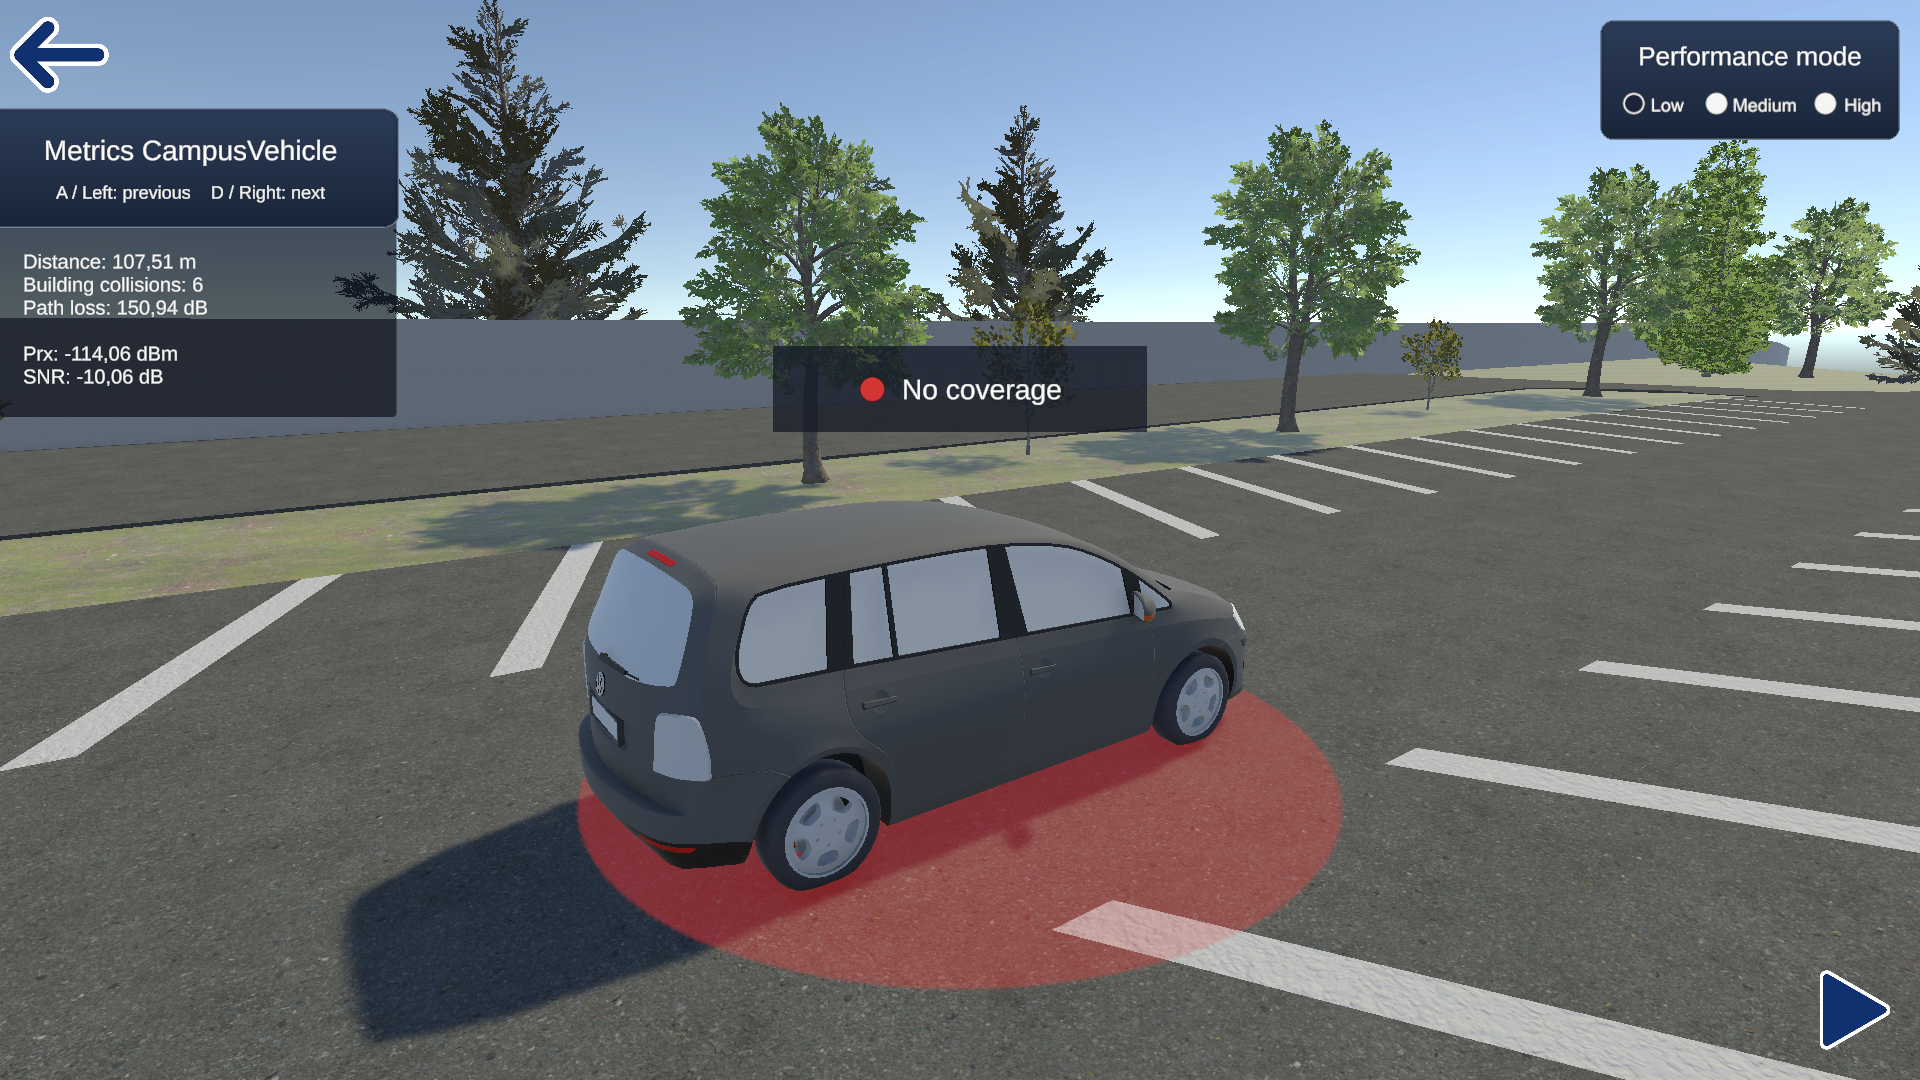
\includegraphics[width=1\textwidth, keepaspectratio]{imagenes/resultados/receptores moviles/vehiculo campus sin cobertura.PNG}
    \caption{Ejemplo de receptor móvil con baja cobertura por obstáculos}
    \label{fig:receptor_baja_cobertura}
\end{figure}

Disponer de un simulador en tres dimensiones permite relacionar los valores numéricos con la posición del receptor dentro del escenario. De esta forma, además de analizar la reducción de potencia en una gráfica, también se puede ver en qué zona del campus se encuentra el receptor y qué elementos del entorno pueden estar afectando al enlace.

Además de mostrar las métricas en tiempo real, el simulador registra los valores calculados durante el recorrido y los exporta posteriormente en archivos CSV. A partir de estos datos se pueden generar gráficas para analizar la evolución de cada receptor. Como ejemplo, en la Figura \ref{fig:linear_vehicle_prx_distance} se muestra la potencia recibida frente a la distancia para el receptor vehicular lineal.

\begin{figure}[H]
    \centering
    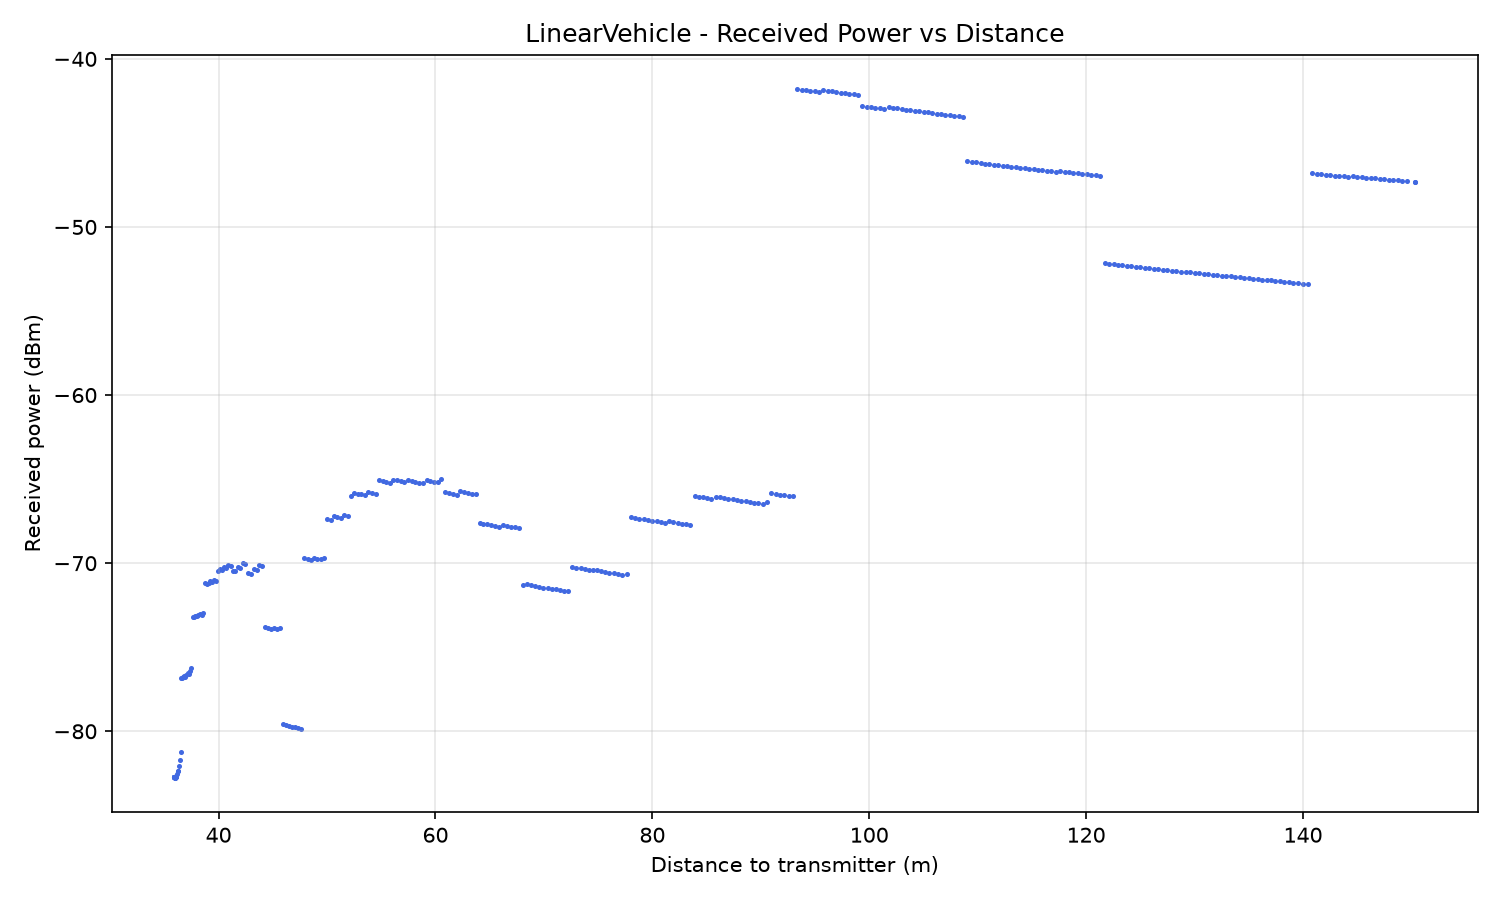
\includegraphics[width=1\textwidth, keepaspectratio]{imagenes/resultados/receptores moviles/30 dbm/LinearVehicle_prx_distance.png}
    \caption{Potencia recibida frente a distancia para el receptor LinearVehicle}
    \label{fig:linear_vehicle_prx_distance}
\end{figure}

En esta gráfica no se observa una disminución uniforme de la potencia recibida con la distancia. Para distancias inferiores a unos 95 m, la señal atraviesa el edificio situado bajo la antena, lo que implica pérdidas adicionales y reduce la potencia recibida. A partir de esa distancia, el receptor deja de estar afectado por esa colisión, y la potencia aumenta de forma brusca. Desde ese punto, la evolución vuelve a ser más progresiva y la potencia tiende a disminuir conforme aumenta la distancia al transmisor. Los saltos menores que aparecen en la gráfica se deben principalmente a los cambios de dirección respecto al patrón de radiación de la antena.

Por tanto, los receptores móviles permiten analizar la cobertura desde dos puntos de vista complementarios. Por un lado, las vistas del simulador muestran en tiempo real la posición del receptor y sus métricas de enlace. Por otro lado, los datos exportados permiten estudiar posteriormente la evolución de esas métricas durante el recorrido. En el siguiente apartado se utiliza esta información para analizar la cobertura según la SNR y los umbrales definidos.

\par\medskip
\textbf{Nota: No sé qué más analizar aquí, tengo varias gráficas aparte de esa pero sería muy repetitivo. Si hay algo más que se os ocurra decídmelo y lo meto.}
\par\medskip


\section{Análisis de cobertura según SNR}

Una vez comprobado el funcionamiento de los receptores móviles, se analiza la cobertura obtenida durante sus recorridos a partir de sus valores de SNR en el tiempo. En este apartado se estudian los resultados de la configuración base y, posteriormente, se aumenta la potencia de transmisión para comparar los cambios en la cobertura resultante.

La comparación se realiza modificando únicamente la potencia de transmisión. Para ello, se utilizan dos valores: 30 dBm, equivalente a 1 W, y 38 dBm, equivalente a 6,31 W. Este último valor corresponde al límite superior definido para una estación base de rango medio según ETSI TS 138 104 \cite{etsi138104}.

Para interpretar los resultados se utilizan los umbrales de SNR configurados en el simulador. En la Figura \ref{fig:snr_time_30dbm} se muestra la evolución temporal de la SNR para el receptor vehicular que recorre el campus utilizando la configuración base de 30 dBm. Se ha elegido este receptor porque su recorrido atraviesa distintas zonas del escenario, dando lugar a más variaciones de cobertura que el resto de receptores móviles.

\begin{figure}[H]
    \centering
    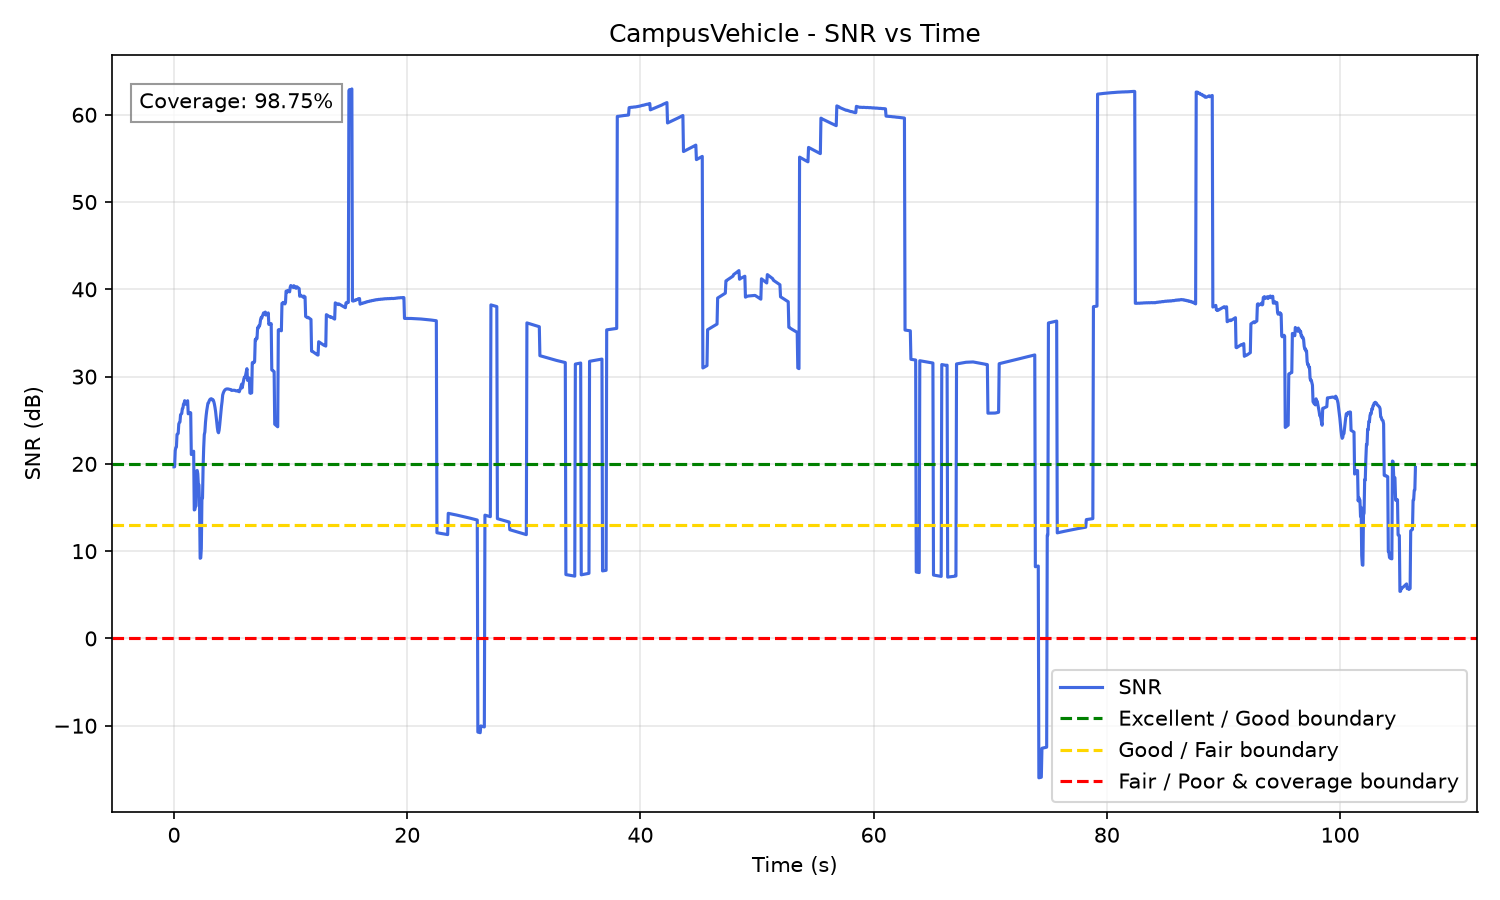
\includegraphics[width=1\textwidth, keepaspectratio]{imagenes/resultados/receptores moviles/30 dbm/CampusVehicle_snr_time.png}
    \caption{Evolución temporal de la SNR con potencia de transmisión de 30 dBm}
    \label{fig:snr_time_30dbm}
\end{figure}

Como se observa, la SNR no se mantiene constante durante el recorrido. Sus variaciones se deben a los cambios de distancia respecto al transmisor, a la orientación respecto al patrón de radiación y a las pérdidas adicionales por las colisiones con edificios.

Al aumentar la potencia de transmisión hasta 38 dBm, la potencia recibida aumenta en todos los puntos del recorrido y, como consecuencia, también mejora la SNR. En la Figura \ref{fig:snr_time_38dbm} se muestra la evolución temporal de la SNR para el mismo receptor utilizando esta potencia superior.

\begin{figure}[H]
    \centering
    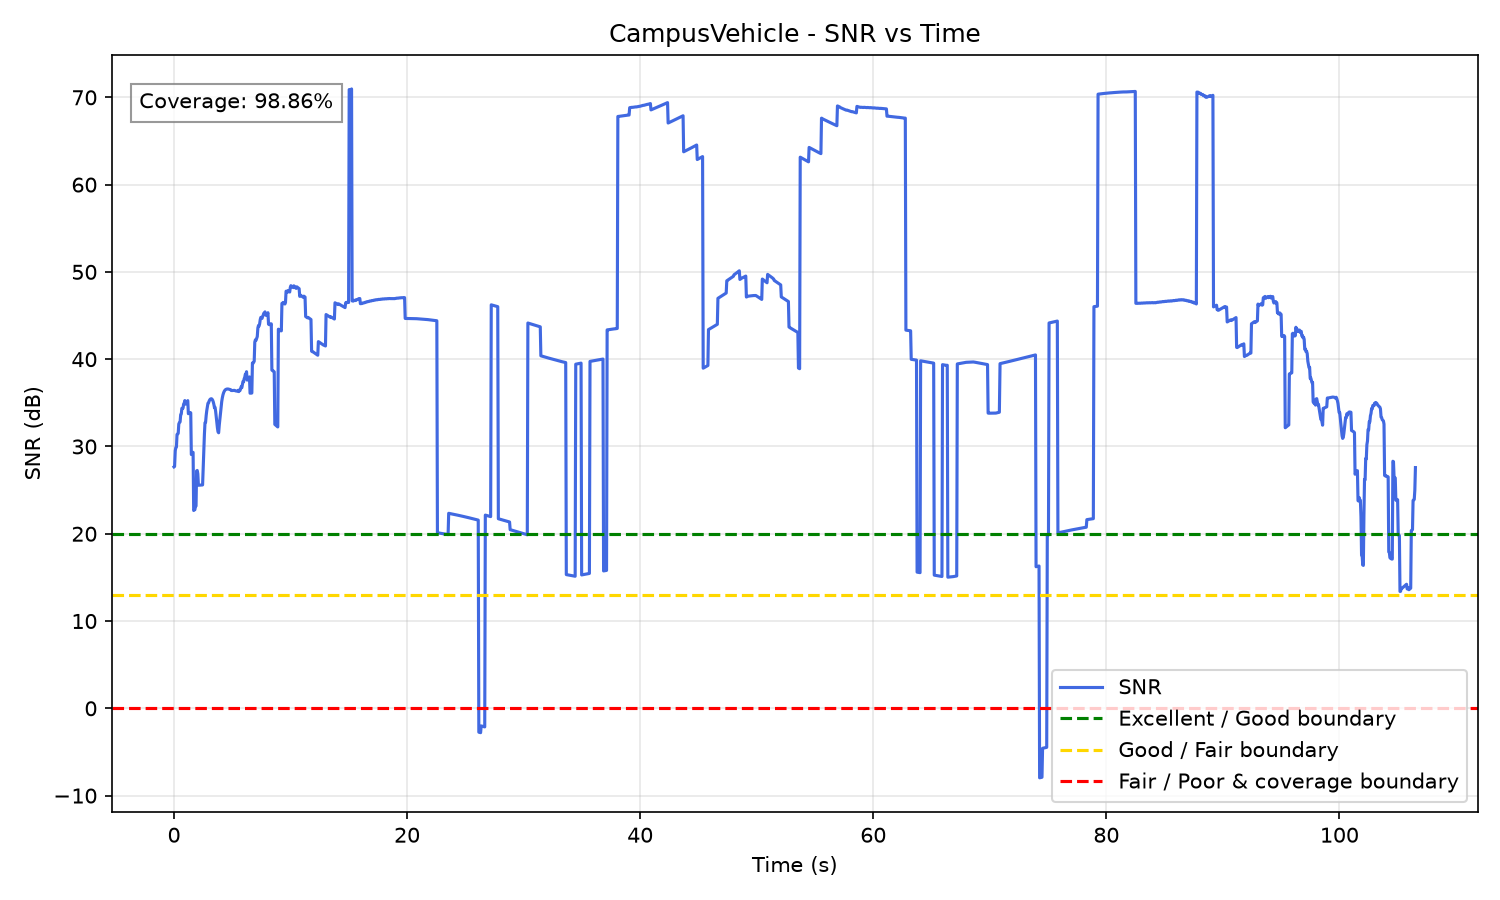
\includegraphics[width=1\textwidth, keepaspectratio]{imagenes/resultados/receptores moviles/38 dbm/CampusVehicle_snr_time.png}
    \caption{Evolución temporal de la SNR con potencia de transmisión de 38 dBm}
    \label{fig:snr_time_38dbm}
\end{figure}

La comparación entre ambas gráficas muestra que el aumento de potencia eleva la SNR durante todo el recorrido. Esto reduce los tramos con cobertura insuficiente y aumenta el porcentaje de tiempo en el que el receptor se mantiene por encima del umbral de cobertura. Sin embargo, las zonas más desfavorables siguen siendo visibles, ya que los obstáculos y las direcciones de menor ganancia del patrón de radiación continúan afectando al enlace.

En la Tabla \ref{tab:cobertura_snr} se muestra el porcentaje de tiempo con cobertura para los tres receptores móviles. Este porcentaje se calcula a partir de las muestras registradas durante el recorrido, considerando como cobertura los instantes en los que la SNR es superior al umbral mínimo establecido anteriormente.

\begin{table}[H]
    \centering
    \begin{tabularx}{\textwidth}{@{}lXX@{}}
        \toprule
        \textbf{Receptor} & \textbf{Cobertura con 30 dBm} & \textbf{Cobertura con 38 dBm}\\
        \midrule
        CampusVehicle & 98,75 \% & 98,86 \% \\
        LinearVehicle & 100 \% & 100 \% \\
        Pedestrian & 100 \% & 100 \% \\
        \bottomrule
    \end{tabularx}
    \caption{Porcentaje de tiempo con cobertura según la SNR}
    \label{tab:cobertura_snr}
\end{table}

Los resultados muestran que, con la configuración base de 30 dBm, la cobertura ya es prácticamente completa en los tres receptores. Tanto el vehículo lineal como el peatón se mantienen por encima del umbral durante todo el recorrido, mientras que el vehículo del campus presenta una pequeña pérdida de cobertura en algunos instantes puntuales. Al aumentar la potencia hasta 38 dBm, esta pérdida se reduce ligeramente, pasando de un 98,75 \% a un 98,86 \%.

La mejora no es muy elevada porque el porcentaje de tiempo con cobertura inicial ya era alto. En este caso, aumentar la potencia no cambia de forma significativa el resultado, pero sí permite comprobar que los puntos más desfavorables del recorrido del vehículo del campus están relacionados con zonas concretas donde coinciden obstáculos y menor ganancia del patrón de radiación. Para eliminar por completo esas caídas, sería necesario seguir aumentando la potencia, aunque esto llevaría a valores menos razonables para el escenario analizado.

Por tanto, este análisis muestra que la configuración base ofrece cobertura suficiente en la mayor parte del campus. La SNR permite detectar los instantes puntuales en los que la cobertura empeora, aunque el porcentaje total siga siendo muy alto. Esto resulta útil porque permite localizar zonas problemáticas que podrían pasar desapercibidas si solo se analizara un valor medio o una visión general del mapa de calor.


\section{Comparación entre configuraciones}

En este apartado se comparan distintas configuraciones del simulador para estudiar cómo afectan algunos parámetros al resultado final. En primer lugar, se analiza el efecto del patrón de radiación utilizado por la antena. Después, se compara el comportamiento obtenido al utilizar dos modelos de pérdidas distintos: FSPL y ABG.

\subsection{Comparación entre patrones de radiación}

Para realizar la comparación, solo se modifica el patrón de radiación utilizado por el simulador. Se utilizan tres patrones diferentes: omnidireccional con ganancia máxima de 16 dBi, reconstrucción mediante el método de Gil y reconstrucción mediante el método de Vasiliadis con $k = 2$.

En la Figura \ref{fig:comparativa_patrones_altura_antena} se muestran los mapas de calor 2D obtenidos para los tres patrones en la capa más cercana a la altura de la antena. Esta comparación permite estudiar cómo varía la distribución de potencia recibida cuando se modifica el patrón de radiación de la antena.

\begin{figure}[H]
    \centering
    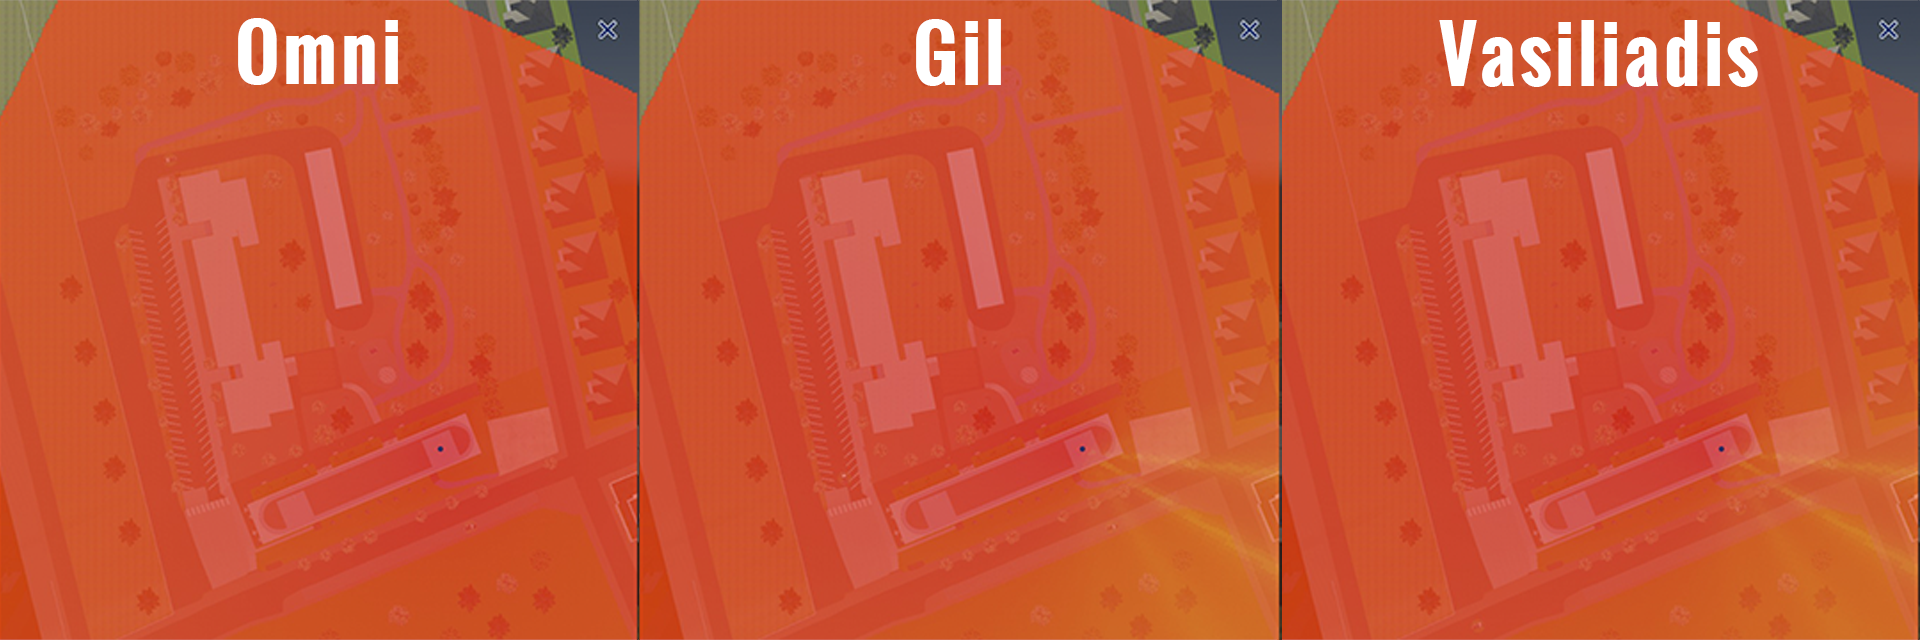
\includegraphics[width=1\textwidth, keepaspectratio]{imagenes/resultados/Comparacion configuraciones/comparacion patrones/comparacion mapas 2d base.png}
    \caption{Comparación de mapas de calor 2D para distintos patrones de radiación a la altura de la antena}
    \label{fig:comparativa_patrones_altura_antena}
\end{figure}

\par\medskip
\textbf{Nota: He puesto dos alturas porque, si no, lo saturaría demasiado de imágenes, aunque lo mejor es verlo en el propio programa y no mediante capturas. Las he recortado para meter tres en una, pero eso hace que no se vea la leyenda, que es un factor importante. La otra opción es poner las tres imágenes completas, una tras otra, pero creo que eso lo saturaría demasiado.}
\par\medskip


En esta capa, las diferencias entre configuraciones son menos evidentes, ya que se trata de una zona cercana a la altura del transmisor y los valores de potencia recibida son elevados en gran parte del mapa. Aun así, se aprecia que el patrón omnidireccional tiene valores altos en todas las direcciones, mientras que los patrones reconstruidos concentran la mayor potencia hacia la parte frontal de la antena. En la zona trasera, tanto Gil como Vasiliadis muestran valores menores, ya que la ganancia del patrón real es menor en dicha dirección.

Para comparar una zona más realista, en la Figura \ref{fig:comparativa_patrones_suelo} se muestra una capa situada cerca del nivel del suelo. Esta altura es más interesante porque se aproxima a la zona donde se encuentran los receptores móviles durante sus recorridos.

\begin{figure}[H]
    \centering
    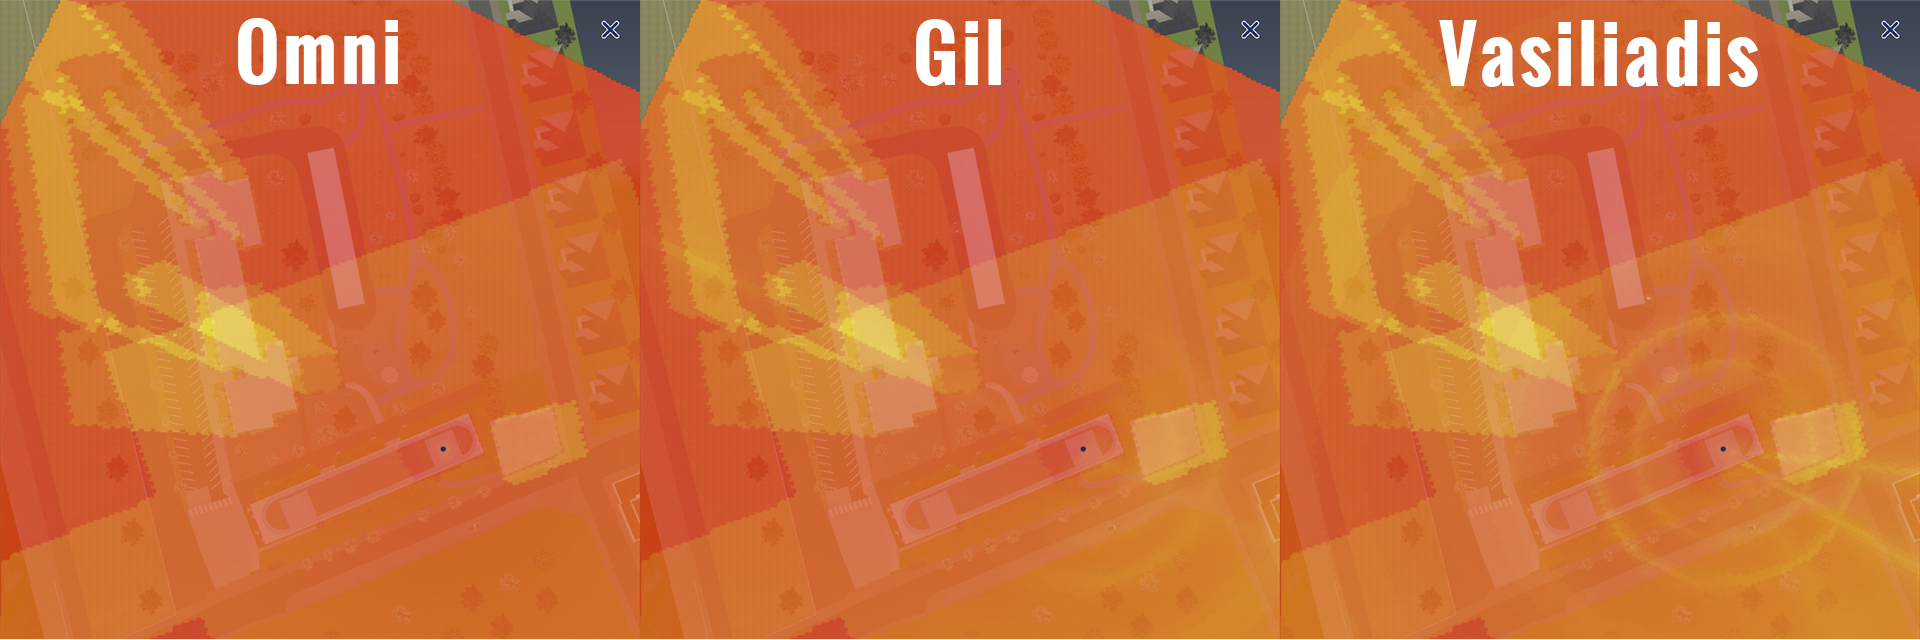
\includegraphics[width=1\textwidth, keepaspectratio]{imagenes/resultados/Comparacion configuraciones/comparacion patrones/comparacion mapas 2d suelo.png}
    \caption{Comparación de mapas de calor 2D para distintos patrones de radiación cerca del nivel del suelo}
    \label{fig:comparativa_patrones_suelo}
\end{figure}

\par\medskip
\textbf{Nota: Realmente no es la altura del suelo, porque al tener un escenario con relieve, el receptor del campus se mueve entre -19 y -25 metros respecto a la antena. Elegí 20 porque es la altura de los otros dos receptores móviles, pero es una aproximación.}
\par\medskip

En la capa cercana al suelo se observan diferencias más claras entre patrones. Con el patrón omnidireccional, la potencia se reparte de forma similar en todas las direcciones, por lo que las zonas de menor potencia se deben a la distancia hasta el transmisor y a las pérdidas introducidas al atravesar edificios.

En cambio, en los patrones reconstruidos aparecen zonas de menor potencia debido a la forma del patrón de radiación. Con Vasiliadis se distinguen varias franjas circulares alrededor de la antena, correspondientes a direcciones con menor ganancia, además de tres haces traseros donde la potencia disminuye de forma notable. En Gil también aparecen variaciones similares, aunque se observan principalmente franjas semicirculares en la parte trasera y con un haz de menor potencia menos marcado.

Además del mapa de calor, se analiza el efecto de cada patrón sobre los receptores móviles. Para ello, se calcula la potencia recibida media durante el recorrido de cada receptor, utilizando los datos exportados en los archivos CSV. Como los valores de potencia están expresados en dBm, primero se convierten a escala lineal en mW, después se calcula la media y finalmente se vuelve a convertir el resultado a dBm. En la Tabla \ref{tab:comparativa_patrones_prx} se muestran los resultados obtenidos para los tres patrones de radiación analizados.

\begin{table}[H]
    \centering
    \begin{tabularx}{\textwidth}{@{}lXXX@{}}
        \toprule
        \textbf{Receptor} & \textbf{Omni} & \textbf{Gil} & \textbf{Vasiliadis} \\
        \midrule
        CampusVehicle & -36,44 dBm & -43,43 dBm & -50,42 dBm \\
        LinearVehicle & -33,94 dBm & -42,91 dBm & -49,87 dBm \\
        Pedestrian & -49,61 dBm & -58,14 dBm & -67,37 dBm \\
        \bottomrule
    \end{tabularx}
    \caption{Potencia recibida media para distintos patrones de radiación}
    \label{tab:comparativa_patrones_prx}
\end{table}

Los resultados permiten comprobar que el patrón de radiación influye fuertemente en la potencia recibida por los receptores móviles. En todos los recorridos, el patrón omnidireccional da lugar a los valores medios más altos. Esto se debe a que, aunque también presenta variación con la elevación, no introduce una diferencia tan marcada entre la parte frontal y trasera de la antena como ocurre con los patrones reconstruidos.

Sin embargo, este resultado no significa que el patrón omnidireccional sea la configuración más realista. Los patrones reconstruidos representan mejor el comportamiento direccional de la antena utilizada, ya que parten de los cortes reales del patrón de radiación. Aunque sus valores medios sean menores, especialmente en el caso de Vasiliadis, estos resultados son más coherentes con una antena real, donde la potencia recibida depende de la dirección concreta en la que se encuentra cada receptor respecto al transmisor.

Por tanto, la comparación muestra que no basta con analizar si existe cobertura o no. Dos configuraciones pueden ofrecer cobertura suficiente en gran parte del recorrido, pero presentar niveles de potencia recibida muy distintos. Por este motivo, la potencia media y los mapas de calor ayudan a interpretar mejor el efecto del patrón de radiación utilizado.

\subsection{Comparación entre modelos de pérdidas}

Además del patrón de radiación, el modelo de pérdidas utilizado también afecta a los resultados obtenidos. Para comprobarlo, se comparan dos configuraciones modificando únicamente el modelo de pérdidas: una utilizando el modelo FSPL y otra utilizando el modelo ABG.

El modelo FSPL representa la propagación en espacio libre, por lo que depende principalmente de la distancia y de la frecuencia. En cambio, el modelo ABG incorpora parámetros dependientes del tipo de escenario y permite representar un comportamiento más específico para entornos urbanos. Por este motivo, se espera que los resultados obtenidos con ABG no coincidan con los obtenidos mediante FSPL.

En la Figura \ref{fig:comparativa_fspl_abg} se muestra la comparación entre ambos modelos de pérdidas para la misma configuración de antena y potencia de transmisión. Para facilitar la interpretación, se utiliza nuevamente la capa más cercana al nivel del suelo.

\begin{figure}[H]
    \centering
    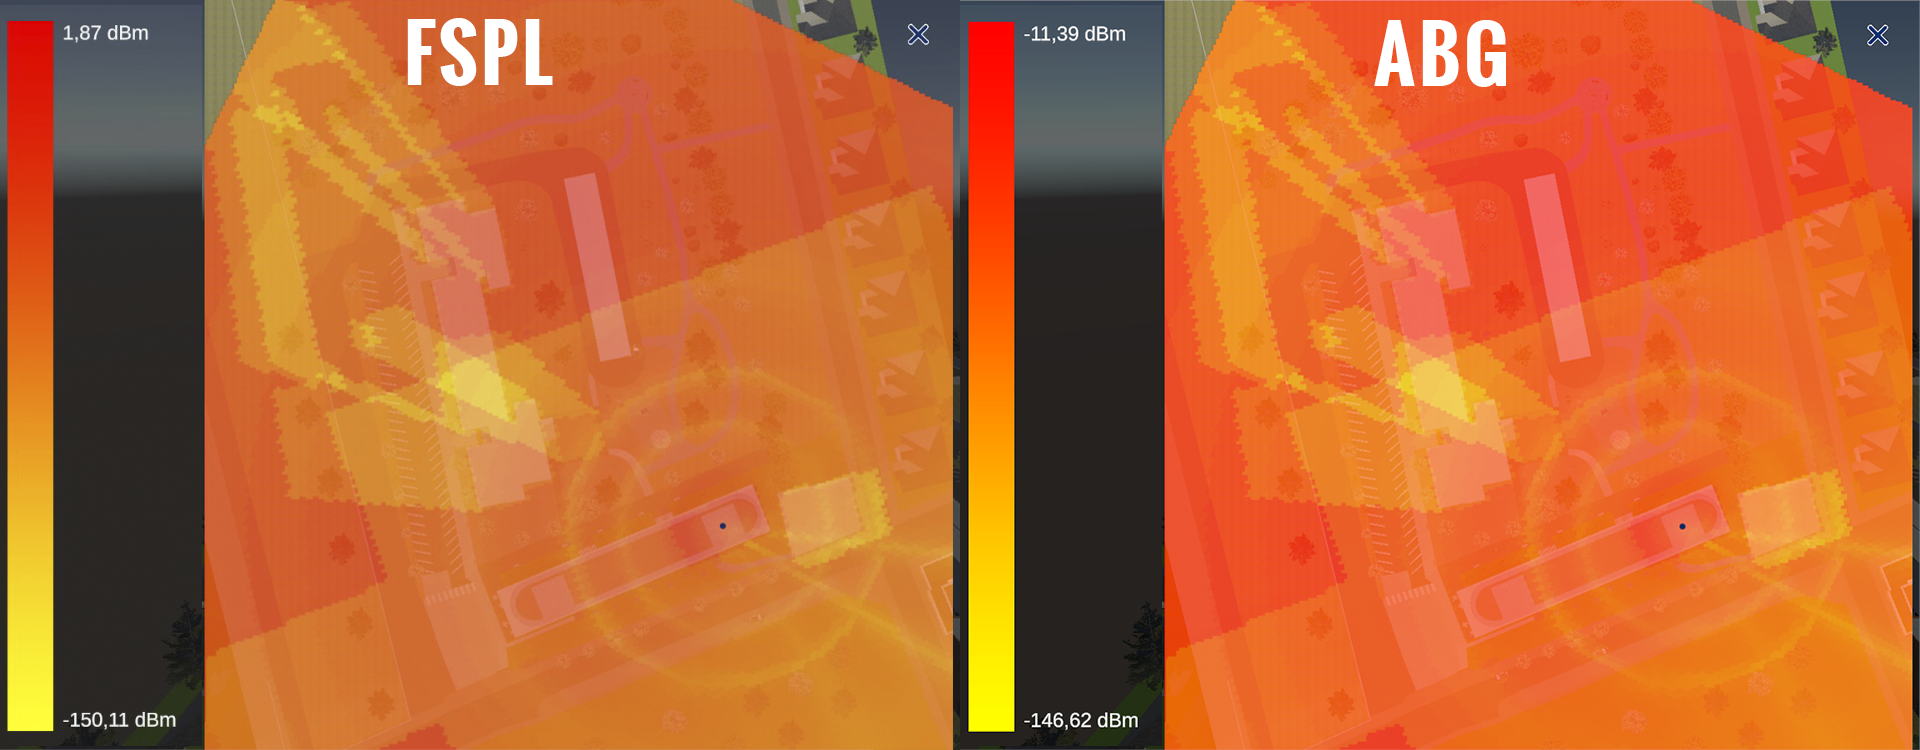
\includegraphics[width=1\textwidth, keepaspectratio]{imagenes/resultados/Comparacion configuraciones/comparacion modelos/Comparacion modelos.png}
    \caption{Comparación de mapas de calor 2D utilizando los modelos FSPL y ABG}
    \label{fig:comparativa_fspl_abg}
\end{figure}

En la comparación visual se observa que la distribución de potencia es similar en ambos modelos. Las zonas de mayor y menor potencia aparecen aproximadamente en las mismas regiones del campus, ya que se mantiene el mismo patrón de radiación, la misma posición de la antena y los mismos obstáculos en el escenario. Sin embargo, los valores límite sí cambian: en FSPL el valor máximo mostrado es de 1,87 dBm, mientras que en ABG es de -11,39 dBm. Los valores mínimos, al contrario, son más cercanos, con -150,11 dBm en FSPL y -146,62 dBm en ABG.

Por tanto, aunque el mapa de calor permite ver que la distribución general es muy similar, no es suficiente para valorar por sí solo cómo afecta el cambio de modelo a los receptores. Para completar la comparación, se calcula la potencia recibida media de cada receptor a partir de los datos exportados en los CSV. Al igual que en el apartado anterior, los valores en dBm se convierten primero a mW, se calcula la media en escala lineal y, finalmente, se vuelve a convertir el resultado a dBm.

\begin{table}[H]
    \centering
    \begin{tabularx}{\textwidth}{@{}lXX@{}}
        \toprule
        \textbf{Receptor} & \textbf{FSPL} & \textbf{ABG} \\
        \midrule
        CampusVehicle & -50,42 dBm & -46,47 dBm \\
        LinearVehicle & -49,87 dBm & -46,10 dBm \\
        Pedestrian & -67,37 dBm & -66,93 dBm \\
        \bottomrule
    \end{tabularx}
    \caption{Potencia recibida media para distintos modelos de pérdidas}
    \label{tab:comparativa_modelos_perdidas}
\end{table}

Los valores de la tabla permiten comparar el efecto de cada modelo sobre los recorridos de los receptores móviles. Aunque en el mapa de calor el valor máximo de ABG es menor que el de FSPL, las potencias medias obtenidas para los receptores vehiculares son superiores con ABG. Esto indica que, aunque el valor máximo del mapa de calor sea mayor, no significa que todas las potencias recibidas lo sean.

En el caso del receptor peatonal, la diferencia entre ambos modelos es mucho menor. Esto se debe a que cada receptor recorre zonas distintas del escenario, con diferentes distancias al transmisor, direcciones respecto al patrón de radiación y colisiones con edificios. Por tanto, el cambio de modelo de pérdidas no afecta por igual a todos los receptores.

Esta comparación muestra que es importante analizar los resultados desde varios puntos de vista. El mapa de calor permite observar la distribución espacial de la potencia, mientras que los datos exportados de los receptores móviles permiten estudiar qué ocurre durante recorridos concretos. Por ello, no es suficiente quedarse solo con la representación visual o con un valor máximo, sino que es necesario combinar ambas fuentes de información.

\par\medskip
\textbf{Nota: He hecho todas las pruebas que hemos ido hablando en las reuniones y que me habéis dicho. Es un poco raro por el tema de que el punto fuerte de este trabajo es la visualización en tiempo real y aquí solo se pueden poner capturas. No obstante, si se os ocurre algo más decídmelo y meto la prueba/datos que me digáis.}
\par\medskip


\section{Limitaciones detectadas}

Aunque el simulador desarrollado permite analizar la cobertura de forma visual y comparar distintas configuraciones, durante las pruebas se han detectado algunas limitaciones que deben tenerse en cuenta al interpretar los resultados:

\begin{itemize}
   \item \textbf{Pérdida asociada a edificios:} las pérdidas por edificios se calculan correctamente a partir de las colisiones detectadas, pero todos los edificios se interpretan como si estuvieran formados únicamente por hormigón. Por tanto, no se diferencian materiales como cristal, metal o ladrillo, ni se tienen en cuenta ventanas, ventanales, puertas o muros interiores. Además, los edificios se consideran huecos, por lo que no se modelan las pérdidas que podrían aparecer al atravesar su interior.
    
    \item \textbf{Resolución de la rejilla de propagación:} para cubrir todo el campus es necesario generar una cantidad de vóxeles muy elevada. Lo ideal sería utilizar un tamaño de vóxel menor para obtener mejores resultados, pero al reducirlo aumentan enormemente los recursos necesarios para llevar a cabo la simulación, pudiendo hacer que deje de ejecutarse correctamente en equipos convencionales. Por este motivo, en las pruebas que cubren todo el campus se utiliza un tamaño de vóxel de 2 m. Este valor permite mantener un coste computacional asumible, pero reduce la resolución de los mapas de calor.

    \item \textbf{Rutas de los receptores móviles:} las métricas de los receptores móviles solo se obtienen en los puntos por los que pasan sus rutas. Esto permite estudiar la evolución de la señal durante recorridos concretos, pero no conocer directamente la potencia recibida en cualquier punto deseado del campus.

    \item \textbf{Reconstrucción aproximada del patrón de radiación:} el patrón tridimensional se obtiene a partir de los dos cortes bidimensionales de la antena. Esto genera una aproximación, pero no equivale a una medida real completa en tres dimensiones. Además, algunos métodos de reconstrucción simplifican la información. Por ejemplo, el método de Vasiliadis trabaja únicamente con 180 grados del patrón, por lo que parte de la información original se pierde durante la reconstrucción.

    \item \textbf{Visualización del mapa de calor:} al representar muchos vóxeles semitransparentes al mismo tiempo, algunas zonas pueden saturarse visualmente y ser difíciles de interpretar. Para reducir este problema, se añadieron controles de transparencia, umbral y mapa 2D por capas, pero la interpretación del mapa sigue dependiendo de la configuración visual elegida por el usuario.
\end{itemize}

\chapter{Conclusiones y trabajos futuros}
\label{chap:conclusiones}

En este capítulo se presentan las conclusiones obtenidas tras el desarrollo y la evaluación del simulador a partir de los objetivos planteados inicialmente. Además, se proponen distintas líneas de trabajo futuro para ampliar sus funcionalidades, mejorar el realismo de la simulación y aumentar las posibilidades de análisis.


\section{Conclusiones}

El estudio de la cobertura es fundamental para analizar el comportamiento de los sistemas de comunicaciones inalámbricas y conocer cómo se distribuye la señal en una zona determinada. Una herramienta tridimensional aporta una ventaja importante, ya que permite relacionar los valores calculados con la posición real de los elementos dentro del escenario. En entornos urbanos, la señal puede verse afectada por muchos factores, como la posición de las antenas, el patrón de radiación, los obstáculos, la altura de los receptores o el modelo de propagación utilizado.

Este tipo de análisis puede realizarse modificando los parámetros de entrada y observando cómo afectan a los resultados obtenidos. En este proyecto se ha desarrollado un simulador tridimensional que representa visualmente la cobertura en un entorno urbano. Para ello, se ha combinado Unity para la parte visual e interactiva con Python para los cálculos de propagación y métricas del enlace.

A partir del desarrollo realizado y de las pruebas obtenidas, se puede concluir que se han cumplido los objetivos planteados inicialmente:

\begin{itemize}
    \item Se ha construido un escenario urbano tridimensional basado en el Centro Universitario de Mérida, incluyendo edificios, vehículos, peatones y elementos del entorno. Esto permite analizar la cobertura en un escenario reconocible y no únicamente en un entorno genérico.

    \item Se ha modelado una antena transmisora con diferentes patrones de radiación. Primero se implementó un modelo omnidireccional y posteriormente se incorporó una antena de tipo panel con un patrón reconstruido a partir de sus cortes horizontal y vertical.

    \item Se ha implementado la reconstrucción tridimensional del patrón de radiación mediante distintos métodos. Las pruebas realizadas frente a MATLAB muestran que la reconstrucción mediante Vasiliadis con k = 2 reproduce exactamente los valores utilizados como referencia, por lo que el método utilizado por el simulador es el mismo que el utilizado en un software real funcional.

    \item Se ha conseguido combinar Unity con el simulador externo desarrollado en Python. Unity se encarga de la interacción, la representación del escenario y la visualización de resultados, mientras que Python realiza los cálculos de propagación y métricas del enlace, como la potencia recibida y la SNR.

    \item Se ha representado la cobertura mediante una rejilla tridimensional de vóxeles y un mapa de calor 3D. Además, se ha añadido una vista 2D por capas de altura, lo que facilita el análisis de la potencia recibida en zonas concretas del escenario y permite estudiar la influencia de la altura.

    \item Se han añadido receptores móviles con rutas definidas dentro del campus. Gracias a ellos, se ha podido analizar la evolución de la cobertura durante el movimiento y comprobar que la señal no depende únicamente de la distancia al transmisor, sino también del patrón de radiación, los obstáculos y la posición del receptor.

    \item Se ha implementado la exportación automática de resultados en CSV y la generación de gráficas. Esto permite conservar los datos de cada ejecución, analizar los resultados fuera de Unity y comparar distintas configuraciones de simulación.

    \item También se han incorporado mejoras de rendimiento para facilitar la ejecución del simulador en equipos con distintas prestaciones. Entre ellas se encuentra la generación del mapa de calor mediante \textit{chunks}, lo que permite dividir la malla en bloques y gestionar mejor su representación. Además, se han añadido modos de rendimiento para ocultar elementos secundarios del escenario cuando sea necesario, junto con una limitación de FPS para evitar un consumo innecesario de recursos.
\end{itemize}

Finalmente, se puede concluir que se han cumplido los objetivos propuestos al inicio del proyecto. El simulador permite configurar distintos escenarios de prueba, representar la cobertura de forma tridimensional, analizar receptores móviles, comparar configuraciones y exportar los resultados obtenidos para su estudio posterior.

\par\medskip
    \textbf{Nota: Yo incluiría aquí una reflexión personal sobre cómo este trabajo ha supuesto un reto y refleja el trabajo de un ingeniero: resolver un problema que requiere combinar conocimientos de distintos campos. Ha sido necesario investigar previamente los conceptos teóricos, construir un escenario 3D, trabajar con un tipo de programación diferente, aplicar técnicas de optimización, diseño... Aunque no sé si esto sobra aquí, si ponerlo en un apartado específico o si no se puede poner ya que es personal y no es neutro formal como el resto del trabajo.}
\par\medskip

\section{Trabajos futuros}

Debido al limitado tiempo del proyecto, no se han podido implementar todas las funcionalidades deseadas. A partir del simulador desarrollado, se plantean varias líneas de mejora que permitirían aumentar el realismo de la simulación, ampliar las posibilidades de análisis y hacer la herramienta más flexible.

\begin{itemize}
    \item \textbf{Pérdidas por materiales:} la primera mejora directa sería implementar los distintos materiales presentes en los edificios, además del hormigón, aplicando pérdidas distintas según el material atravesado. Además, podrían añadirse pérdidas adicionales al propagarse por el interior de los edificios, ya que ETSI TR 138 901 incluye tanto pérdidas por penetración en materiales como una pérdida interior dependiente de la profundidad dentro del edificio \cite{etsi138901}.

    \item \textbf{Receptor móvil controlable por el usuario:} otra mejora muy útil sería añadir un receptor que pueda moverse libremente por el escenario. Esto permitiría consultar la cobertura en puntos concretos elegidos por el usuario, en lugar de depender únicamente de rutas predefinidas. Esta funcionalidad requeriría implementar control de movimiento y físicas, ya que el escenario tridimensional cuenta con relieve y sería necesario gestionar correctamente las colisiones con el suelo, la gravedad y el desplazamiento del receptor sobre el terreno.

    \item \textbf{Modificación de la posición de la antena:} actualmente la antena se encuentra en una posición fija dentro del escenario. Como trabajo futuro, sería interesante permitir modificar su ubicación desde la interfaz, para estudiar cómo cambia la cobertura al colocar el transmisor en distintos puntos del campus.

    \item \textbf{Múltiples tipos de antenas:} actualmente el simulador permite utilizar una antena omnidireccional y una antena de tipo panel reconstruida a partir de sus cortes horizontal y vertical. Como mejora futura, podrían añadirse más tipos de antenas reales, permitiendo cargar y reconstruir patrones con características distintas. Esto permitiría comparar antenas con diferentes ganancias y patrones de radiación dentro del mismo escenario.

    \item \textbf{Incorporación de varias antenas transmisoras:} otra línea de mejora sería permitir el uso de más de una antena en el escenario. Esto permitiría estudiar cómo cambia la cobertura al añadir varios transmisores, analizar zonas cubiertas por más de una antena e introducir interferencias entre ellas.

    \item \textbf{\textit{Beamforming:}} también podría añadirse algún tipo de \textit{beamforming}. Esta técnica permite concentrar la energía transmitida o recibida en una dirección concreta mediante un array de antenas, aumentando la ganancia respecto a una transmisión omnidireccional \cite{7342886}. En el simulador, esto permitiría orientar dinámicamente el haz de radiación hacia determinadas zonas o receptores, estudiando técnicas más cercanas a sistemas celulares actuales.

    \par\medskip
    \textbf{Nota: Esto lo leí en el TFG que me pasasteis como referencia y José Javier dijo que podíamos estudiarlo llegado el momento, pero jamás llegamos a volver a hablarlo, por lo que lo he metido como trabajo futuro. He cogido la referencia del TFG para sacar la definición también de ahí.}
    \par\medskip

    \item \textbf{Reconstrucción del patrón mediante \textit{deep learning}:} una mejora futura sería añadir un método de reconstrucción basado en \textit{deep learning}. MATLAB utiliza esté método mediante la función \texttt{patternFromAI}, que permite reconstruir un patrón tridimensional a partir de dos cortes bidimensionales utilizando un modelo preentrenado \cite{mathworks_patternfromai}. Esto podría mejorar la reconstrucción en antenas con patrones más complejos, donde los métodos tradicionales como Gil o Vasiliadis pueden perder información.
\end{itemize}

 

% --- Bibliografía ---
\addcontentsline{toc}{chapter}{Referencias}
\pagestyle{plain}

%  carpeta 'bibliografia'
%se llame 'referencias.bib'
\nocite{*}
\bibliography{bibliografia/referencias}{} 
\bibliographystyle{ieeetr} % Estilo de ingeniería (números [1], [2])

% --- Anexos ---
\appendix
\chapter{Uso responsable de herramientas de inteligencia artificial}
\label{anexo:uso_ia}

Durante el desarrollo de este trabajo, se han utilizado herramientas de inteligencia artificial generativa como apoyo en distintas tareas. Una de ellas ha sido la búsqueda de referencias útiles, ya que ChatGPT no solo permite buscar información, sino también localizar fuentes a las que acudir para consultarla.

Además, estas herramientas han resultado realmente útiles durante el desarrollo en Unity, ya que permiten obtener de forma rápida explicaciones sobre el funcionamiento del motor y resolver dudas que, de otro modo, habrían requerido depender de foros, vídeos o tutoriales. También se han utilizado para obtener ideas sobre el diseño y la distribución de los elementos de la interfaz. Este apoyo ha sido fundamental en la elección de colores debido al daltonismo del autor.

\par\medskip
\textbf{Nota: Queda un poco raro decir daltonismo del autor, pero no puedo hablar en primera persona de mí; no sé como decirlo de otra forma.}
\par\medskip

La memoria se ha redactado en Overleaf, que incluye una herramienta de corrección automática mediante inteligencia artificial. Esta función ayuda a detectar problemas de puntuación, especialmente relacionados con el uso del punto y coma, y propone cambios para mejorar la formalidad y la claridad de la redacción, de una forma similar a los correctores ortográficos habituales de Word.

También se han utilizado estas herramientas para comprender conceptos nuevos relacionados con las distintas áreas del proyecto. Algunos artículos presentaban una dificultad elevada, y mantener una conversación con una inteligencia artificial generativa ha permitido comprender mejor determinados conceptos mediante explicaciones más sencillas y adaptadas a cada duda.

En ningún caso la inteligencia artificial sustituye el trabajo del ingeniero, ya que las decisiones, la implementación y la comprobación de los resultados siguen siendo responsabilidad del autor. Sin embargo, utilizada de forma crítica y responsable, puede ser una herramienta de gran utilidad para adquirir conocimientos.


\par\medskip
\textbf{Nota: Fui a ver las presentaciones de los TFGs de informática de julio, y el tribunal les preguntó directamente cómo habían usado la IA en el trabajo, ya que en la memoria no lo aclaraban. No sé si esto queda demasiado forzado, ya que algunos profesores son anti IA, pero como lo hablamos en una reunión, lo dejo aquí.}
\par\medskip

\end{document}